%!TEX TS-program = xelatex
%!TEX encoding = UTF-8 Unicode

%%
%% 南京大学物理学院 2012级 曾培 本科毕业论文
%% Github主页:https://github.com/qubiter
%%

%% 使用 njuthesis 文档类生成南京大学本科生毕业论文的示例文档
%% 作者:张楚珩,zhangchuheng123 (at) live (dot) com
%% 个人主页: http://sealzhang.tk
%%

%% 如需Adobe字体请用(默认)
%\documentclass[adobefonts]{njuthesis}
%% MacOS系统请用
%\documentclass[macfonts]{njuthesis}
%% Windows系统请用
\documentclass[winfonts]{njuthesis}
%% Linux系统请用
%\documentclass[linuxfonts]{njuthesis}

\usepackage{CJKulem}  %for Chinese underline
\usepackage{listings} %for code highlights \begin{lstlisting}
\usepackage{xcolor}   %for listings color
\usepackage{setspace} %for space setting

%%%%%%%%%%%%%%%%%%%%%%%%%%%%%%%%%%%%%%%%%%%%%%%%%%%%%%%%%%%%%%%%%%%%%%%%%%%%%%%
% 设置论文的中文封面
% 论文标题
\title{一种深度学习网络的测试与专用电路设计}

% 论文作者姓名
\author{曾培}
% 论文作者学号
\studentid{121120171}
% 导师姓名职称
\supervisor{王中风}
\supervisortitle{教授}
% 论文作者院系
\department{物理学院}
% 论文作者的学科与专业方向
\major{物理学院\;物理系}
% 论文作者的研究方向
\researchfield{深度学习\; 数字电路 \;量子信息}
% 论文作者的年级
\grade{2012级}
% 论文的定稿日期,需设置年、月、日。此属性可选,默认值为最后一次编译时的日期,精确到日。
\date{2016年5月23日}
\submitdate{2016年5月23日}

%%%%%%%%%%%%%%%%%%%%%%%%%%%%%%%%%%%%%%%%%%%%%%%%%%%%%%%%%%%%%%%%%%%%%%%%%%%%%%%
% 设置论文的英文封面

% 论文的英文标题
\englishtitle{Algorithm Test and A Digital Circuit Design of The DeSTIN Deep Learning Frame}
% 论文作者姓名的拼音
\englishauthor{ZENG Pei}
% 导师姓名职称的英文
\englishsupervisor{Prof. WANG Zhongfeng}
% 论文作者所在院系的英文名称
\englishdepartment{Department of Physics}
% 论文作者所在学校或机构的英文名称。此属性可选,默认值为``Nanjing University''。
\englishinstitute{Nanjing University}
% 论文完成日期的英文形式,默认最后一次编译的时间
\englishdate{May 23rd, 2013}



\begin{document}
%%%%%%%%%%%%%%%%%%%%%%%%%%%%%%%%%%%%%%%%%%%%%%%%%%%%%%%%%%%%%%%%%%%%%%%%%%%%%%%%
% listings setting
\lstset{numbers=left,
numberstyle=\tiny,
frame=single,
keywordstyle=\color{blue!70}, 
commentstyle=\color{red!50!green!50!blue!50},
rulesepcolor=\color{red!20!green!20!blue!20}, 
breaklines = true, 
basicstyle=\footnotesize\ttfamily,
xleftmargin=1em,xrightmargin=1em,aboveskip=1em,
framexleftmargin=5pt,
framexrightmargin=5pt,
%escapeinside=`,
}



% 制作中文封面
\maketitle
% 制作英文封面

%控制页
\controlpage

% 论文的中文摘要
\begin{abstract}
我们的研究基于一种新型的深度学习框架:深度空时关系推断网络DeSTIN(Deep SpatioTemporal Inference Network)-- 这种框架基于一种神经网络结构(Deep Belief Neural Network),通过实时的k-means聚类方法提取特征,逐步提取出高维输入信息内部的有效全局特征,并对其进行监督学习,从而对新的输入进行有效预测。这种神经网络的优点在于数据的实时更新,可以反映出数据的空时依赖关系。

我们首先研究了DeSTIN算法在算法层次上面的具体实现方法,进行了参数调试;然后进行了相应的定点数测试;之后再利用集成电路设计的方法,设计出一种专用的数字电路进行这种神经网络结构的实现。我们通过Verilog HDL进行编程,设计出专用数字电路的结构,进行了相应的仿真工作,确认了我们的设计的合理性。 

我们探讨了其在图像处理上的应用,尤其是对于视频中的动作识别 (空时相关的模式)进行深入研究。

% 中文关键词。关键词之间用中文全角分号隔开,末尾无标点符号。
\keywords{深度学习;模式识别;专用电路}
\end{abstract}

%%%%%%%%%%%%%%%%%%%%%%%%%%%%%%%%%%%%%%%%%%%%%%%%%%%%%%%%%%%%%%%%%%%%%%%%%%%%%%%
% 论文的英文摘要
\begin{englishabstract}
Our research is based on a brand new frame for deep machine learning(DML): the Deep SpatioTemporal Inference Network(DeSTIN). The DeSTIN is constructed based on the former work of Deep Belief Neural Network and Deep Neural Network. We adopt the online k-means clustering method for the neuron learning process, and with a network of clustering structure, we can extract the feature from different level, which can be used for latter pattern recogition.

The Strengthness of this algorithm is that 1) It's much faster and feasible comparing to other kinds of Deep Neural network; 2) It can extract the spatialtempral information effectively; 3) It's relatively easy for transplant to digital circuit.

We first did some research on the algorithm hierarchy: how it can work on some normal learning database; and check it's robustness and limitation on each kind of learning problem; then we finished the fixed point test with MATLAB; finally we designed the digital circuit's structure, programmed with Verilog, and do the simulation on Modelsim platform.
% 英文关键词。关键词之间用英文半角逗号隔开,末尾无符号。
\englishkeywords{Deep Machine Learning, Pattern Recognition, Digital Circuits}
\end{englishabstract}

%%%%%%%%%%%%%%%%%%%%%%%%%%%%%%%%%%%%%%%%%%%%%%%%%%%%%%%%%%%%%%%%%%%%%%%%%%%%%%%
% 论文的前言,应放在目录之前,中英文摘要之后
%
\begin{preface}

(初稿暂无序言部分的内容)


\vspace{1cm}
\begin{flushright}
曾培\\
2016年5月22日于南京大学
\end{flushright}

\end{preface}

%%%%%%%%%%%%%%%%%%%%%%%%%%%%%%%%%%%%%%%%%%%%%%%%%%%%%%%%%%%%%%%%%%%%%%%%%%%%%%%
% 生成论文目录
\tableofcontents

%%%%%%%%%%%%%%%%%%%%%%%%%%%%%%%%%%%%%%%%%%%%%%%%%%%%%%%%%%%%%%%%%%%%%%%%%%%%%%%
% 生成插图清单。如无需插图清单则可注释掉下述语句。
\listoffigures

%%%%%%%%%%%%%%%%%%%%%%%%%%%%%%%%%%%%%%%%%%%%%%%%%%%%%%%%%%%%%%%%%%%%%%%%%%%%%%%
% 生成附表清单。如无需附表清单则可注释掉下述语句。
\listoftables

%%%%%%%%%%%%%%%%%%%%%%%%%%%%%%%%%%%%%%%%%%%%%%%%%%%%%%%%%%%%%%%%%%%%%%%%%%%%%%%
% 开始正文部分
\mainmatter

%%%%%%%%%%%%%%%%%%%%%%%%%%%%%%%%%%%%%%%%%%%%%%%%%%%%%%%%%%%%%%%%%%%%%%%%%%%%%%%
% 学位论文的正文应以《绪论》作为第一章
\chapter{绪论}\label{chapter_introduction}
\graphicspath{{chapter1/figure/}}
%\bibliographystyle{unsrt}

\section{研究背景}

本论文的研究主要基于两大背景:\uline{Moore定律的最终终结}以及\uline{脑科学,人工智能研究的兴起}。

Moore定律是由Intel的创始人Gordon Moore于1965年提出的一个经验规律,其描述的内容是:在价格不变的情况下,集成电路上可容纳的元件的数目,约每隔18-24个月便会增加一倍,性能也因此提升一倍。\cite{wikipedia_moores_law}

\begin{figure}[htbp]
   \centering
   
\includegraphics[width=0.5\textwidth]{MooreLaw.png} % requires the graphicx package
   \caption{Moore定律:CPU中随着时间指数级增长的晶体管规模}
   \label{fig:moore}
\end{figure}

Moore定律是近50年来信息技术得以迅速发展的重要保障,如图\ref{fig:moore},伴随着晶体管规模的增长,由CPU体现的计算机运算能力也实现了指数级增长,由此促使了人类生活发生了巨大变化。

然而,随着微纳加工逐渐逼近极限,传统的硅基集成电路已经做到尺寸小于10nm的时候,由于加工成本的提升,热效应逐渐明显和量子隧穿效应的出现,传统半导体工艺发展集成电路已经走到了尽头。Gordon Moore于2015年已经公开宣称:“Moore定律十年以内将要结束。”\cite{moore2015declare}

与此同时,人们对于计算的需求却在日益增加。于是,人们从算法、电路、硬件各个层面上探讨如何高效地提升计算能力。一种常见的方法是,改变以前的计算机组织架构,引入一些专用的计算单元来加速某些特定需求的计算。一个常见的专用计算模块便是GPU(Graphics Processing Unit),其通过大量的并行计算结构和有效的内存分配,可以有效地处理图形渲染,矩阵运算等任务。\cite{wikipedia_gpu}

常见的计算任务除了大量的矩阵运算、图形渲染以外,还有一种日益增长的需要,就是进行模式识别与机器学习,譬如人脸识别、指纹识别、数据预测等等。于是,一种专门适用于进行模式识别、机器学习的电路模块可以很好地平衡通用性与计算效率的需要,有很大的市场需求。

另一方面,随着神经科学、认知心理学和计算机科学的不断进步,人工智能领域的发展十分迅速。

从生物学上来讲,由于研究方法、实验手段日益成熟(荧光成像、核磁共振成像、脑电波),人们对于大脑的神经结构有着日益完善的了解,由此展开的类脑结构计算,脑机接口的研究不断深入;IBM的TrueNorth研究团队\cite{brainchip2014}对于电路搭建实现类脑结构已经做出了喜人的结果。(图\ref{fig:truenorth})
从计算机科学上来讲,在神经科学的启发下,通过结合统计学、统计物理的研究成果,一门新兴的学科——机器学习产生了广泛的应用。

\begin{figure}[htbp]
   \centering
   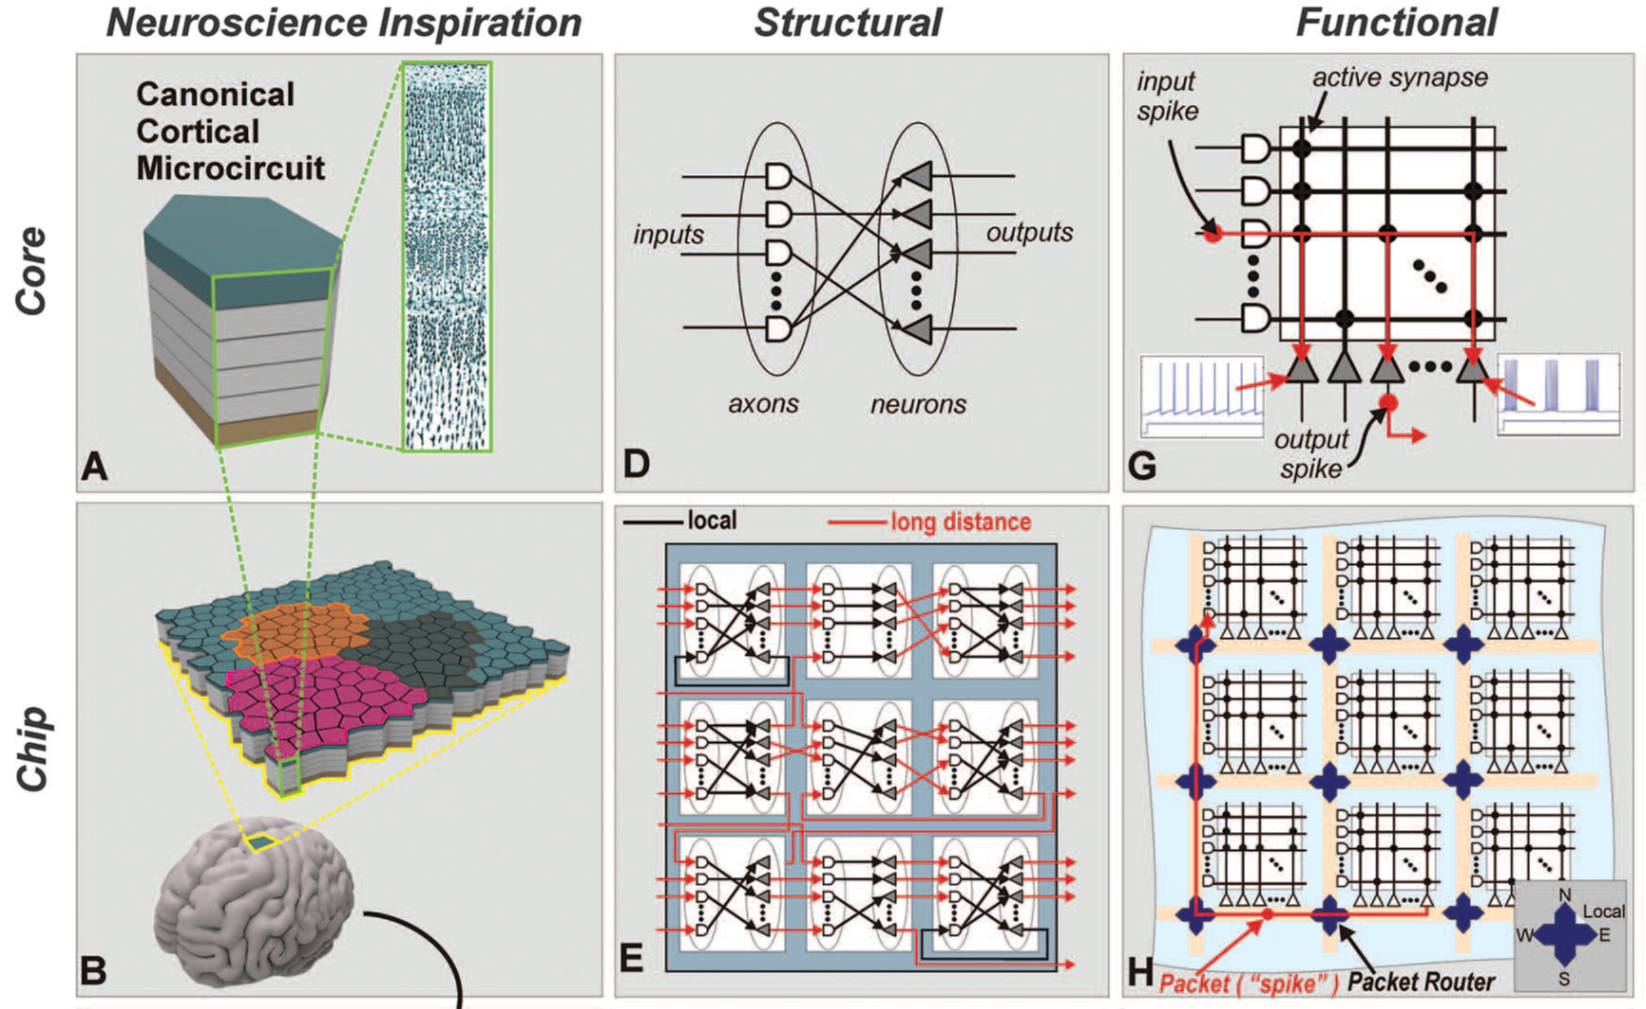
\includegraphics[width=0.7\textwidth]{TrueNorth.png} % requires the graphicx package
   \caption{TrueNorth类脑结构实现原理}
   \label{fig:truenorth}
\end{figure}

综合以上两个方面,人们想通过专用电路的设计实现特定的模式识别功能;并以此为基础,搭建类脑的神经网络,研究类脑结构的计算框架。

\section{研究目的与意义}
\subsection{现有解决方法}
在专用电路进行机器学习领域,中科院计算技术研究所的陈天石,陈云霁等人推出的“寒武纪”处理器系列处于国际领先的地位\cite{Chen2014DianNao},其设计的“DianNaoYu”指令集能够很好的实现卷积神经网络(Convolutional Neural Network)和深度神经网络(Deep Neural Network)的通用架构设计。图\ref{fig:diannao}为其“DianNao”处理器内部的实现加速的硬件架构。

\begin{figure}[htbp]
   \centering
   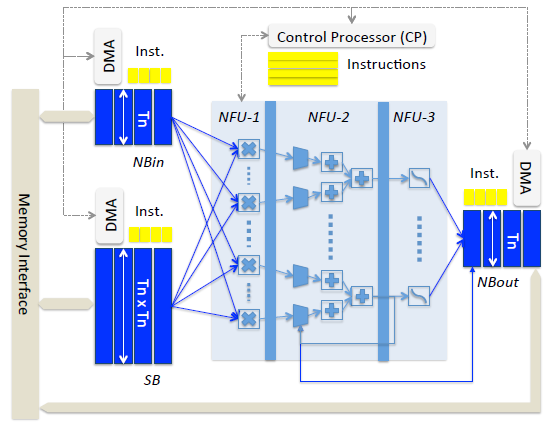
\includegraphics[width=0.6\textwidth]{DianNao.png} % requires the graphicx package
   \caption{"寒武纪"系列电脑采用的硬件模块设计}
   \label{fig:diannao}
\end{figure}

除了利用数字电路进行网络架构设计以外,利用模拟电路搭建“模拟神经元”的方法也得到了相关的研究。图\ref{fig:clustering}\cite{Lu2014An}为一种聚类算法的神经元的模拟电路架构。

\begin{figure}[htbp]
   \centering
   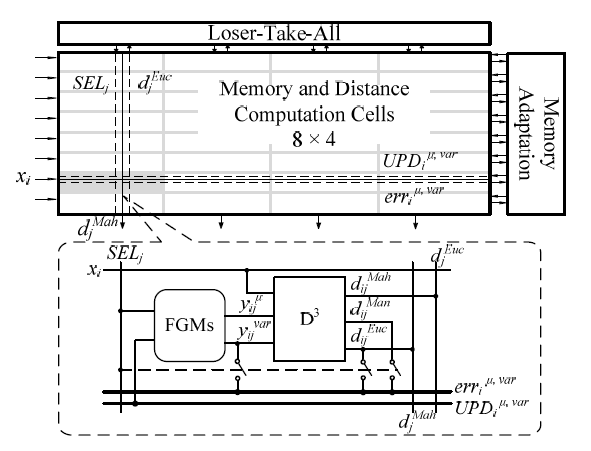
\includegraphics[width=0.6\textwidth]{OnlineClustering.png} % requires the graphicx package
   \caption{Online Clustering算法的模拟神经元架构}
   \label{fig:clustering}
\end{figure}

“寒武纪”系列以及相关的基于卷积神经网络的专用电路方法具有一定的局限性。卷积神经网络应用于静态图像处理取得了巨大成功,但是其在处理时间依赖的问题上面具有严重的局限性。

\subsection{本研究的目的与意义}
本研究试图研究一个对于动态识别具有良好效果的深度学习算法(DeSTIN),先对其算法进行可靠性研究,判断其对于静态、动态图像的识别能力;然后对该算法进行量化,判断其转换为定点数算法之后的可行性;再对该算法进行专用的数字电路设计,并对其进行仿真测试与综合。

在学习算法上,DeSTIN算法相比较于卷积神经网络算法具有本质上的动态识别特性,能够更好更快地进行动态识别处理;与此同时,通过识别扫描的方法,DeSTIN算法能够有效地处理静态图像的识别问题。

与此同时,DeSTIN算法具有并行特性以及参数设置上对于数字电路设计的天然优势。 通过专用数字电路的设计,比较于普通的CPU架构编程实现的算法,我们可以通过减少程序读取、转译,数据传送过程的时间损耗,高效率地使用存储;硬件计算具有天然的并行特性,加上流水线结构实现能够使得整个学习过程较为高效。 

而相对于模拟电路设计实现而言,数字电路设计架构相对简单,具有通用性、可移植性;数字电路可以在前期通过量化的方法进行模拟测试,有成熟的数字电路仿真测试软件,便于综合。

%\bibliography{reference}
\chapter{机器学习与深度学习简介}\label{chapter_machinelearning}
\graphicspath{{chapter2/figure/}}
\bibliographystyle{unsrt}

本章笔者将对机器学习领域的一些基本思想做一个介绍,尤其是介绍与本文算法相关的背景知识。在机器学习的基础上,笔者将对目前深度学习的一些主流方向做一个简介。

\section{机器学习}

\subsection{机器学习简介}

\subsubsection{定义与引例}

机器学习被定义为一门“让计算机在没有被准确、具体地编程的情况下获得学习能力”的学科。
机器学习鉴于一种朴素的思想:\uline{通过机器自动分析数据中的规律,并作出相应的预测}。 

一个最简单的“学习”案例便是曲线的的“拟合”过程。笔者想通过一个“拟合”实例来说明机器学习的基本思想。

假设我们有两个实值变量x、t,其满足关系
\begin{equation}
\label{eqn:random}
y = \sin(2\pi x) + \epsilon
\end{equation}

其中$\epsilon$是一个服从Gaussian分布的随机值。

假设我们有m组(x,y)的观测值$x \equiv (x_1, x_2, ..., x_m)^T, y \equiv (y_1, y_2, ..., y_m)^T$,图\ref{fig:fitting}为m=10时的数据点和原Sine函数。

\begin{figure}[htbp]
   \centering
   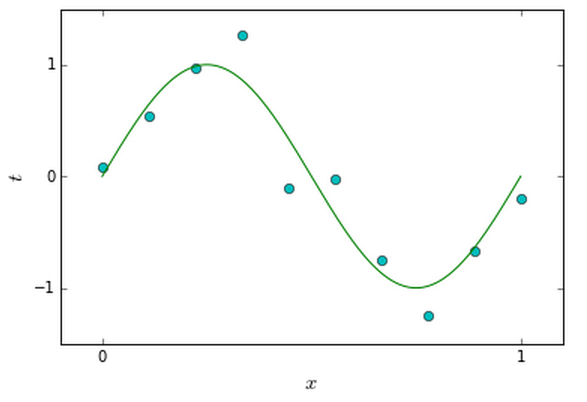
\includegraphics[width=0.5\textwidth]{SineFitting.png} % requires the graphicx package
   \caption{拟合的原数据点,真实的Sine函数}
   \label{fig:fitting}
\end{figure}

图\ref{fig:polyfitting}通过三阶多项式函数进行拟合的结果。通过已知的10个数据点,我们获得了一条多项式曲线,通过这条曲线便可以推断、预测已知数据点之外的点的信息。

\begin{figure}[htbp]
   \centering
   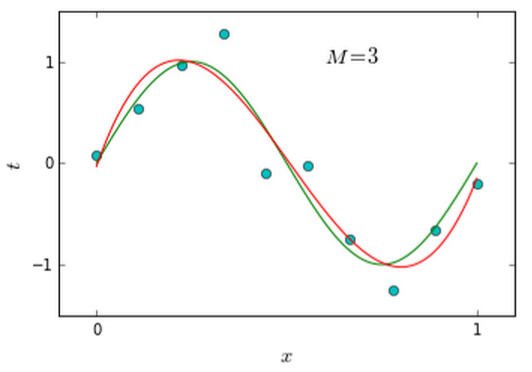
\includegraphics[width=0.5\textwidth]{PolyFitting.png} % requires the graphicx package
   \caption{多项式“拟合”:对真实情况进行预测、推断}
   \label{fig:polyfitting}
\end{figure}

在本例中,机器的学习过程便转化为了\uline{如何产生合适的拟合曲线的问题}。我们假设多项式满足以下形式:
\begin{equation}
h(x,\mathbf{w}) = w_0 + w_1x + w_2x^2 + ... + w_Mx^M = \sum_{j=0}^M w_j x^j
\end{equation}

其中$h(x,\mathbf{w})$为假设预测值,M为多项式阶数,$\mathbf{w} = (w_0, w_1, ..., w_M)$ 表示多项式的系数。

首先,我们就要对曲线“\textbf{合适}”的概念做一个分析。什么是合适的曲线?一个自然的观点便是,曲线应当能够\uline{较好地符合已有的数据}。为了衡量曲线符合已有数据的程度,我们根据曲线预测值和真实值的偏差的函数进行描述。一种常见的偏差的度量是采用\uline{偏差的平方值}(取平方值加和是严格基于数据独立同分布,围绕真实值正态分布的极大似然概率推导得出的\cite{standford_machine_learning_cs229})。于是,我们定义\textbf{损失函数}如下:

\begin{equation}
E(\mathbf{w}) = \dfrac{1}{2} \sum^m_{i=1} (h(x, \mathbf{w}) - y_i )^2
\end{equation}

其中$\frac{1}{2}$是为了之后计算的方便而加上的。

我们的目标便从拟合曲线转变为了\uline{选择合适的$\mathbf{w}$,使得损失函数$E(\mathbf{w})$最小}。

常见的一种方法是,分析此损失函数$E(\mathbf{w})$的梯度,发现其为$\mathbf{w}$的线性函数,即存在唯一极小值点,此即我们寻找的最优点:

\begin{equation}
\dfrac{\partial E(\mathbf{w})}{w_j} = \sum^m_{i=1} ( \sum^m_{j=0} w_j x^j_i - y_i ) x^j_i = 0
\end{equation}

上式即“最小二乘法”的基本原理公式。

然而,在大多数时候,我们的损失函数不具有以上良好的结构:具有多个极小值点;微分性质不佳;甚至没有明确的函数定义。 

于是我们产生了一种基于“学习”的思想:

\uline{先寻找一个或者多个试探点$\{w_j\}$; 再衡量其损失函数的表现; 最后根据原来试探点的表现更新试探点的位置}。 

进行以上迭代,直到得到一个满足要求的点为止。

在以上“学习”过程中,有几个不可或缺的要素:
\begin{itemize}
\item 学习的任务T(Task):在以上实例中,任务的确认即为\uline{描述什么是“合适”的曲线}:函数预测值和原训练点的满足程度;
\item 结果的观测P(Performance):以上实例中,即为\uline{损失函数$E(\mathbf{w})$的具体形式的确定};
\item 学习的经验E(Experience):实例中体现为:\uline{拟合函数形式的假设}(多项式函数)以及\uline{更新规则的制定}。
\end{itemize}

一个被广泛引用的机器学习的定义是\cite{mitchell1997machine}:假设存在一个任务T,已有的经验E,和对于结果的观测P;如果一个机器通过经验E改善了其在任务T中的表现(通过P来观测),我们就说机器进行了学习。


%最早的机器学习研究源于统计学里面的一些方法:回归分析、主元分析、聚类问题、Bayesian推断等等。 

相比较于普通的静态算法(比如最小二乘法)而言,机器学习更加看重“数据驱动”(data-driven),根据数据变化不断调整自己的推断、预测。


\subsubsection{机器学习的分类}
机器学习按照学习形式主要划分为\uline{监督学习、非监督学习}两大类。其主要的区别就在于学习的任务T(Task)的区别:

\begin{itemize}
\item 监督学习中,训练数据集含有训练的标签值(比如说实例中的y值);学习的任务一般为\uline{提高函数预测值$h_i$和原训练点标签值$y_i$的满足程度};
\item 非监督学习中,训练数据集不带有标签;学习的任务可能为:寻找数据的聚类;主元分析等等。(后面会展开讲)
\end{itemize}

除了以上的两类机器学习,还存在着\uline{半监督学习、强化学习}的学习类型。

半监督学习指的是数据集中存在一部分数据具有训练标签(往往更加贴近于实际情况),而大部分数据是没有标签的情况下进行数据分析预测; 

强化学习是目前的一个新兴领域,其主要思想是结果的观测P不再基于具体的损失函数$E(\mathbf{w})$,而是基于一个刺激信号(比如下围棋时获得胜利能够赢得奖励)。

本章主要围绕较为成熟的监督学习、非监督学习理论展开介绍。

\subsection{监督学习}
根据上一节,我们已知,监督学习为提高函数预测值$h_i$和原训练点标签值$y_i$的满足程度
 根据数据集的具体形式,监督学习可以具体表现为:
\begin{enumerate}
\item 回归问题: 数据集的自变量X、因变量y(标签)\textbf{均连续};
\item 分类问题: 数据集的自变量X\textbf{连续},因变量y(标签)\textbf{离散};
\item 序列标记问题: 数据集自变量X、因变量y(标签)\textbf{均离散};
\end{enumerate}
以下我们主要讨论回归问题与分类问题。 

我们先分析常规回归问题的处理方法,再讨论利用Sigmoid函数实现分类问题的处理;当自变量X维数增加时,应用常规的高维优化方法将变得非常困难,我们将讨论基于此发展的神经网络算法,这将是后来深度学习算法的重要基础;最后我们将简要地介绍机器学习的基本数学基础:Bayes理论。

\subsubsection{优化方法之梯度下降法}
我们将回归问题进一步抽象:为了不失普遍性,我们设自变量有两个,因变量有一个;数据空间为($y: x_1, x_2$)。训练集为m组数据($y_i: x_{1i}, x_{2i} (i=1\sim m)$)。 

那么任何一个回归问题都可以分为三个部分:

\begin{enumerate}
\item 数据结构的先验假设: y与x的函数关系假设; 最终将会被抽象为一个线性表达式

\begin{equation}
\begin{aligned}
h(x,\mathbf{w}) = & w_0 + w_{10} x_1 + w_{20} x_1^2 + ... + w_{M0} x_1^M + w_{01} x_2 + w_{02} x_2^2 + ... \\
& + w_{0N} x_2^M + w_{11} x_1 x_2 + ...+ w_{ij} x_1î x_2^j + ... + w_{k} f(x_1, x_2)
\end{aligned}
\end{equation}

其中y表示为$x_1$, $x_2$的幂指数项,$x_1, x_2$的交叉幂项,以及某些先验的$f(x_1, x_2)$非幂项(比如$\sqrt{x_1}$)。

\item 损失函数$E(\mathbf{w})$形式的确认: 对于回归问题,我们采用训练集真实数据$y_i$同模型预测值$h_i$的差值的平方和作为损失函数。 更加严格地,为了防止“过拟合”现象的发生,我们在损失函数后附上正则化项
\begin{equation}
\label{eqn:costfunction}
E(\mathbf{w}) = \dfrac{1}{2} \sum^N_{i=1} (y_i(x, \mathbf{w}) - t_i )^2 + \dfrac{\lambda}{2} ||w||^2
\end{equation}

\item 损失函数极小化采用的优化方法。 比如前面提到的利用一阶导数为0寻找极小值点的最小二乘法。
\end{enumerate}

本小节我们讨论另外一种常见的优化方法:\textbf{梯度下降法}。梯度下降法代表了含导数优化方法的典型思想,在机器学习优化中被广泛应用。

梯度下降的基本思想是:不断地更新$\mathbf{w}$使$E(\mathbf{w})$变小;利用导数去判别更新$\mathbf{w}$的方向和长度,逼近极值点的位置。具体的更新规则为:

\begin{equation}
w_j := w_j -\alpha \dfrac{\partial}{\partial w_j} E(\mathbf{w})
\end{equation}

其中$\alpha$称为\uline{学习速率},是一个人为的参数。

在一个梯度下降进行学习的过程中,我们基于当前的$\mathbf{w}$进行预测值h的计算,并且计算其损失函数$E(\mathbf{w})$;再由损失函数及其梯度更新$\mathbf{w}$;循环以上步骤,直到满足停止条件(比如w基本不变)为止。


对于公式\ref{eqn:costfunction}形式的损失函数,其导数值为:
\begin{equation}
\dfrac{\partial}{\partial w_j} E(\mathbf{w}) = \dfrac{\partial}{\partial w_j} (\dfrac{1}{2} \sum^m_{i=1} (h_i(x, \mathbf{w}) - y_i )^2 + \dfrac{\lambda}{2} w_j^2 =\\
 \sum^m_{i=1} (h_i(x, \mathbf{w}) - y_i ) \dfrac{\partial}{\partial w_j} h_i(x, \mathbf{w}) + \lambda w_j
\end{equation}

我们通过以上梯度下降法和较为普适的线性模型,就可以较为方便地进行低维度回归问题的学习了。更严格的回归问题讨论详见\cite{standford_machine_learning_cs229}。

在基于一阶导数的优化方法中,有很多基于梯度下降法而发展出的方法。如“共轭梯度法”、“BFGS”法,“L-BFGS”法,他们往往比梯度下降法更快,并且不容易进入局部极小值点。在此不赘述。\cite{wikipedia_BGFS_algorithm}

\subsubsection{Sigmoid分类实现方法}
本节我们讨论分类问题的处理方法。 我们首先讨论二分类问题,即数据标签${t_i}$只有两种取值的情况。不失普遍性,我们假设${t_i}$取值为0或者1。

我们仍然可以套用之前回归模型的处理方法:仍然假设$E(\mathbf{w}) = \dfrac{1}{2} \sum^m_{i=1} (h_i(x, \mathbf{w}) - y_i )^2 + \dfrac{\lambda}{2} ||w||^2$,其中$y_i$的值取0或者1;通过$h_i(x,\mathbf(w))$表达式的值来确定h的大小。 然而,实验证明这样的效果并不理想,h的值不能总是很好地收敛于0,1旁边,训练处的模型y值较为分散。

一种朴素的改进方案是,不再通过连续值$h_i$来表示预测值,而是对其进行\textbf{后处理},将其处理成\uline{间断值}。比如说,设置一个变量$d_i$,其定义为:
\begin{equation}
d_i(h_i(x,\mathbf{w})) == \left\{
\begin{aligned}
 & 1  & h_i > 0.5 \\
 & 0  & h_i < 0.5 \\
\end{aligned}
\right.
\end{equation}

此模型称为“感知机”模型。\cite{wikipedia_perceptron}历史上“感知机”模型曾经是分类的主流方法。 

然而,此方法的缺点非常明显:\uline{$d_i(h_i)$不是一个微分性质良好的函数,不能够进行梯度下降法的优化计算}。

基于此,我们想到了用一个接近于“感知机”,但具有良好微分性质的函数来后处理$h_i$,这样便能得到较好的分类结果。

一个常见的“分类”函数称为Sigmoid函数,其表达式为:
\begin{equation}
d_i(h_i) = \dfrac{1}{1+e^{-d_i}}
\end{equation}

为了统一符号,我们在此改变符号记法,用$h$表示最终的预测值(即处理后的d值),而用$z$表示后处理之前的线性加和值(原h值),即:
$$ h(x,\mathbf{w}) = h(z(x,\mathbf{w})) = g(z) = \dfrac{1}{1 + e^{-z}}$$

其形状如图所示:

\begin{figure}[htbp]
   \centering
   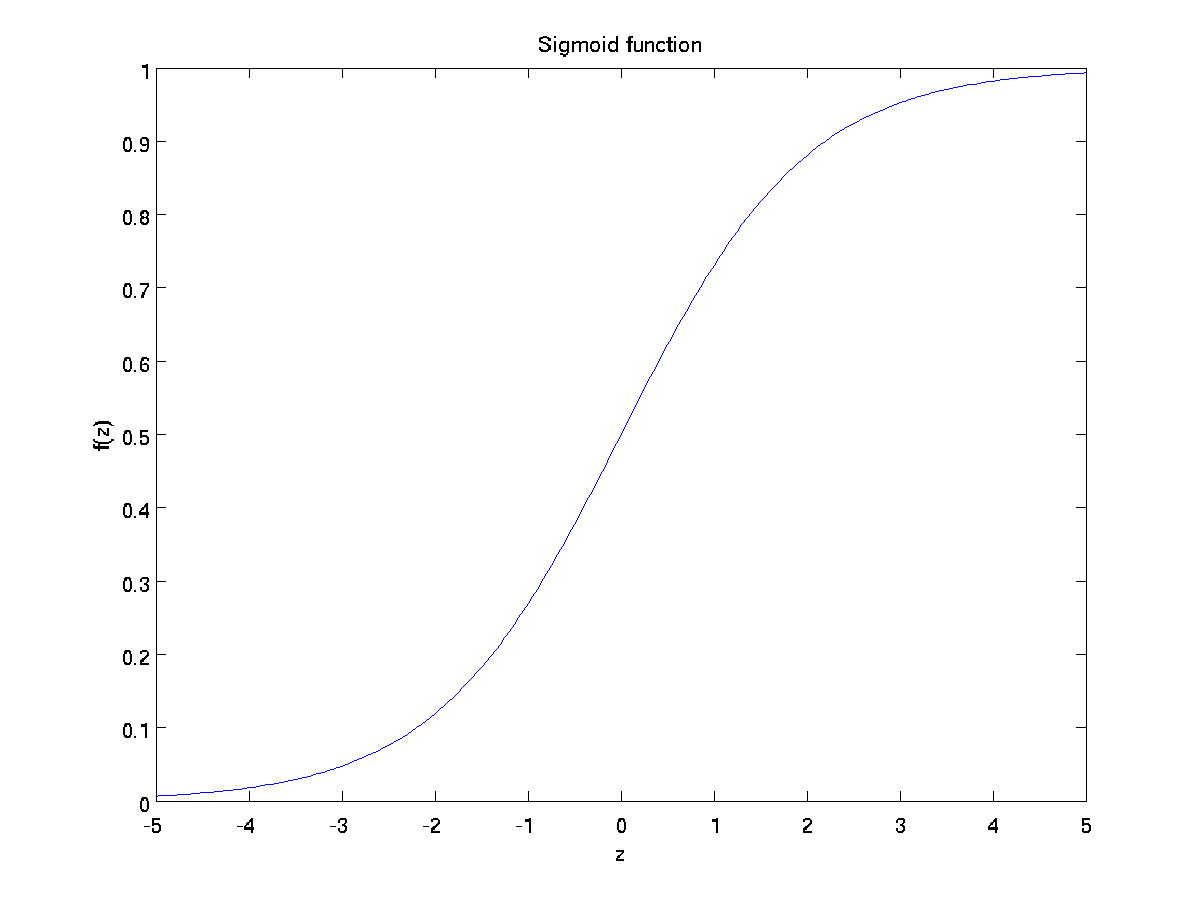
\includegraphics[width=0.6\textwidth]{SigmoidFunction.png} % requires the graphicx package
   \caption{Sigmoid函数的形状}
   \label{fig:sigmoid}
\end{figure}

我们称,$h$的值表示其归为分类‘1’的可信度。相反,其归为‘0’的可信度表示为$1 - h$。可见,当$z$大于0时,$h$的值大于0.5;反之$h$的值小于0.5。

那么,在训练的过程中,我们用$h$替代$z$作为优化的因变量,损失函数写为:(仍然通过极大似然法求得,考虑先取对数\cite{standford_machine_learning_cs229})

\begin{equation}
\begin{aligned}
& E(\mathbf{w}) = \dfrac{1}{m} \sum^m_{i=1} Cost(h(x^{(i)}),y^{(i)}) \\
& Cost(h(x^{(i)}),y^{(i)}) = \left\{
\begin{aligned}
 & -log(h(x))   & y = 1 \\
 & -log(1-h(x)) & y = 0 \\
\end{aligned}
\right.
\end{aligned}
\end{equation}

损失函数的图像如下:
\begin{figure}[htbp]
   \centering
   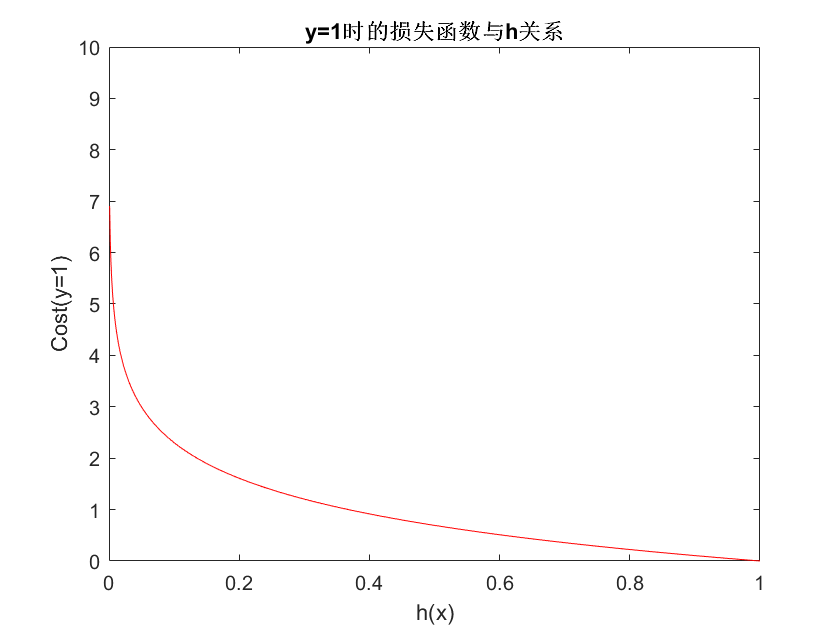
\includegraphics[width=0.6\textwidth]{SigmoidCost1.png} % requires the graphicx package
   \caption{Cost函数与h的关系(y=1)}
   \label{fig:sigmoidcost1}
\end{figure}

\begin{figure}[htbp]
   \centering
   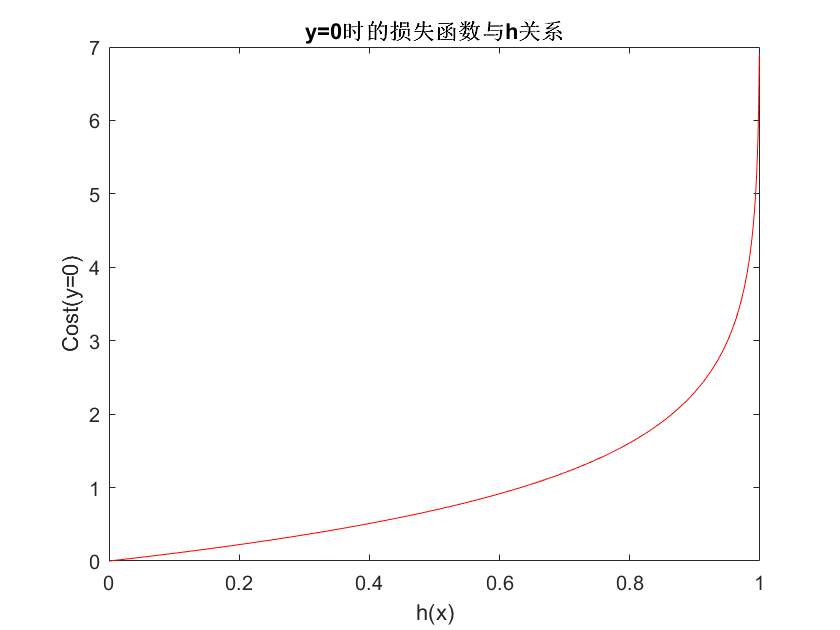
\includegraphics[width=0.6\textwidth]{SigmoidCost0.png} % requires the graphicx package
   \caption{Cost函数与h的关系(y=0)}
   \label{fig:sigmoidcost0}
\end{figure}

可见当$y=1$时,函数一边趋向于0,一边趋向于无穷大;反之亦然。那么,根据其表达式,损失函数可以进一步化简合并为:
\begin{equation}
E(\mathbf{w}) = -\dfrac{1}{m} \sum^m_{i=1} [y^{(i)}log(h(x^{(i)},\mathbf{w})) + (1 - y^{(i)})log(1 - h(x^{(i)},\mathbf{w})) ]
\end{equation}

相应地,我们可以求其一阶导数的表达式如下:(具体推导略)

\begin{equation}
\dfrac{\partial}{\partial w_j} E(\mathbf{w}) = \sum^m_{i=1} (h(x^{(i)}) - y^{(i)})x^{(i)}_j
\end{equation}

这样我们就可以利用之前总结的梯度下降法或者相应的方法进行权重值$\mathbf{w}$的训练。

在进行预测时,如果$y_i>0$,我们则预测相应自变量x对应分类`1';反之预测其对应分类`0'。 

对于多类别的分类问题,我们可以简单地将其划归为多个二分类问题进行处理(称为one-VS-all方法):

比如,当标签$y\in {0,1,2,...,n}$时,我们可以建立一组假设:
$$
\begin{aligned}
h^{(0)}(x,\mathbf{w}) & = & P(y=0|x;\theta)\\
h^{(1)}(x,\mathbf{w}) & = & P(y=1|x;\theta)\\
...\\
h^{(n)}(x,\mathbf{w}) & = & P(y=n|x;\theta)\\
\end{aligned}
$$
最终的预测值$pred = arg\, max_i (h^{(i)}(x))$。

分类问题有很多种解决方法: Softmax函数方法,k-means分类法,支持向量机(Support Vector Machine)方法,决策树方法\cite{standford_machine_learning_cs229};其体现的精神实质是大致相同的,在此就不一一赘述了。

\subsubsection{神经网络}
以上我们讨论了回归、分类问题最具代表性的处理方法。然而,我们可以发现以上模型在面对较高维度输入的时候面临着一些困难: 我们以回归问题为例,当自变量X的具有100维度时,我们考虑先验的$y(x_1, x_2, ..., x_100)$包含项的数目。 我们假设每一个幂项的最高指数为10,没有任何先验的非线性项,那么表达式
\begin{equation}
\begin{aligned}
y(x,\mathbf{w}) = & w_0 + w_{10} x_1 + w_{20} x_1^2 + ... + w_{M0} x_1^M + w_{01} x_2 + w_{02} x_2^2 + ... \\
& + w_{0N} x_2^N + w_{11} x_1 x_2 + ...+ w_{ij} x_1î x_2^j + ... + w_{k} f(x_1, x_2)
\end{aligned}
\end{equation}
中至少有:$100^{10}$项。 

我们发现,随着问题输入规模的扩大,学习的复杂度(体现在权重值$\mathbf{w}$的维度上)呈指数增加的态势。 传统的统计优化方法不再直接适用。

这时,计算机科学家转向了生物学寻求帮助。 生物学上来讲,人类大脑接收信息的维度都极其之高:举例来说,视网膜的分辨率可以达到每英寸300$\sim$400个像素点,然而大脑可以低功耗、低处理成本地进行视觉处理。 大脑里面神经的处理方法很值得我们进行借鉴学习。

生物学研究表明,大脑内部的神经连结成一个复杂的网络;对于大多数神经元,存在多条突触结构与其他神经元相连接,当某一条突触结构上(树突)产生一个高位电信号\textbf{高过一定阈值}时,神经元被激活,通过轴突向其他神经元传播电信号。突触的结构会因为刺激信号的强弱而不断受到训练,神经元之间的连接程度会有所改变。

基于以上规律,我们将讨论一种重要的模型结构——\textbf{神经网络},这是后面深度学习处理的基础。 我们先考虑一个最简单的二层神经网络。
\begin{figure}[htbp]
   \centering
   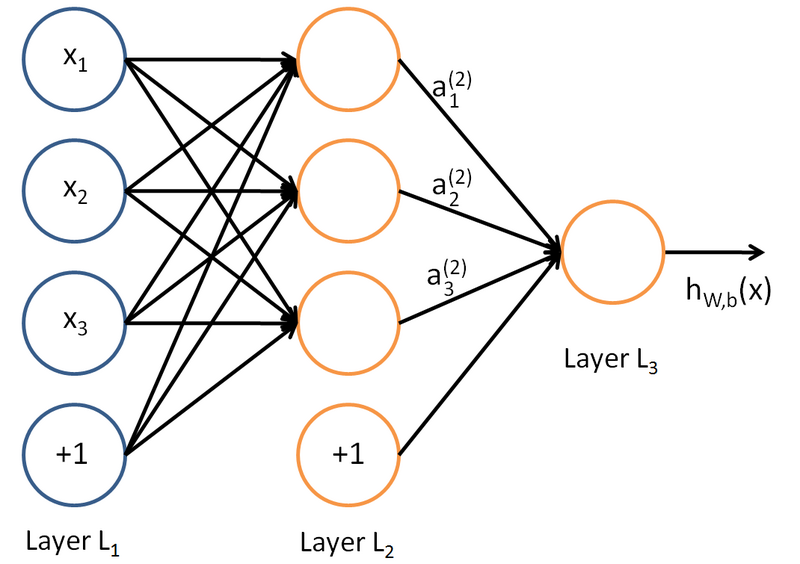
\includegraphics[width=0.7\textwidth]{NeuralNetwork.png} % requires the graphicx package
   \caption{二层神经网络结构示意}
   \label{fig:neuralnetwork}
\end{figure}


如图\ref{fig:neuralnetwork},$a^{(1)}$为输入层,其接收输入信号$x = {x_1, x_2, ... x_{N-1}}$,以及附加一个偏置的常数神经元$a^{(1)}_0$。

$a^{(2)}$为中间层,其中每一个神经元(除了偏置神经元)都与输入层的神经元建立了连接关系,我们假设输入层第$i$个神经元与中间层第$j$个神经元之间的联系权重为$w^{(1)}_{j,i}$。权重值反映两个神经元之间的连接情况:$w^{(1)}_{j,i}=0$反映出两个神经元之间没有连接,$w^{(1)}_{j,i}=1$(归一化以后)反映出两个神经元有很强的正连接关系。其归一化以后的取值范围应当为$[-1,1]$。

我们为了模拟\uline{过阈值激活}的过程,通过sigmoid函数建立起中间层神经元信号强度$a^{(2)}$与输入层信号输入的关系:
\begin{equation}
z^{(2)}_j = \sum^{N_1}_{i = 0} w^{(1)}_{j,i} a^{(1)}_i,\;\; a^{(2)}_j = g(z^{(2)}_j )
\end{equation}
当输入层神经信号的加和值$a^{(2)}_j$超过了阈值“0”的时候,神经元表现为被激活的状态,$z^{(2)}_j$值为1。反之则未激活。

$a^{(3)}$为输出层,其与中间层的连接关系类似与前两层的连接关系:
\begin{equation}
z^{(3)}_j = \sum^{N_2}_{i = 0} w^{(2)}_{j,i} a^{(2)}_i,\;\; a^{(3)}_j = g(z^{(3)}_j )
\end{equation}

神经网络可以应用于回归问题或者是分类问题。

对于一个输入变量x为100维,输出变量y为1维的回归问题,我们可以设置输入层神经元个数$N_1$为100(不包括偏置神经元),用于对应输入$x_1,...,x_100$,设置输出层神经元个数$N_3$为1,中间层设置神经元个数可以自己进行优化,一般设置为$\sqrt{N_1 N_3}$,即设置为10个神经元。 输出层的输出位置我们不再加入Sigmoid函数进行处理,而是直接输出中间层的加和结果:$y = \sum^{N_2}_{i=0} w^{(2)}_{i} a^{(2)}_i$。

此时我们\uline{不再设置各种高阶幂项、交叉项与非线性项的输入},这正是神经网络方法的优势:\uline{sigmoid函数能够较好地处理非线性问题}。通过这样的方法,即使没有高维度的输入变量的假设形式(各种高阶幂项、非线性项),也能够得到较好的结果。在此就不深入探讨原因了,详见\cite{standford_machine_learning_cs229}中的有关讨论。

对于一个输入变量x为400维,标签y为10维的回归问题,应该有:$N_1 = 400, N_2 = 30, N_3 = 10$,此时我们在输出端也加上Sigmoid函数,通过取\uline{输出值里面最大的值}的方法进行预测。

以上我们介绍了利用神经网络的基本结构,以及通过向前传播进行回归、分类预测的方法;然而,如何训练权重值呢? 限于篇幅原因,我们不详细展开讨论,只将结果列出:

首先,神经网络的整体损失函数具体形式为:
\begin{equation}
\begin{aligned}
E(\mathbf{w}) & = [\dfrac{1}{m} \sum^m_{i=1} E(w;x^{(i)},y^{(i)})] + \dfrac{\lambda}{2} \sum^{L-1}_{l=1} \sum^{N_l}_{i=1} \sum^{N_{l+1}}_{j=1} (w^{(l)}_{j,i})^2 \\
& = [\dfrac{1}{m} \sum^m_{i=1}(\dfrac{1}{2}||h(x^{(i)},\mathbf{w})-y^{(i)}||^2)] + \dfrac{\lambda}{2} \sum^{L-1}_{l=1} \sum^{N_l}_{i=1} \sum^{N_{l+1}}_{j=1} (w^{(l)}_{j,i})^2
\end{aligned}
\end{equation}

其中l表示层序数,L为总层数(此处L=3)。$E(w;x^{(i)},y^{(i)})$

为了展开优化,我们需要求出整体损失函数的导数。损失函数对于不同层的导数值求解难易不同,最后一层的w值导数可以直接求得,而E对于前面的每一层w的导数值需要知道后面层数导数值的结果。

因此,我们采用一种“反向传播”的方法求解$E$对于每一层的$w^{(l)}_{j,i}$的导数值\cite{deep_learning_ufldl},具体步骤如下:
\begin{enumerate}
\label{enu: backprop}
\item 由当前的$w^{(l)}_{j,i}$值和输入的$x_i$值进行神经网络的前向传导,得到每一层的激活值$a^{(l)}_j$;
\item 根据输出层的激活值(即预测值$h(x)$)和标签值y计算最后一层的残差:
\begin{equation}
\delta^{(L)}_i = \dfrac{\partial}{\partial z^{(i)}_i} \dfrac{1}{2} ||y - h(x,\mathbf{w})||^2 = -(y_i - a^{(L)}_i) \cdot g^\prime (z^{(L)}_i)
\end{equation}
其中g(z)为Sigmoid函数。那么我们已知其导数值:$g^\prime(z^{(l)}_i) = g(z^{(l)}_i)(1-g(z^{(l)}_i)) = a^{(l)}_i(1-a^{(l)}_i)$。
\item 由最后一层逐层反向计算$l = L-1, L-2, ...2$各层的残差值:
\begin{equation}
\delta^(l) = (\sum^{N_{l+1}}_{j=1}(w^{(l)}\delta^{(l+1)})) \cdot g^\prime (z^{(l)}_i)
\end{equation}
\item 由每层的残差计算相应的导数值:
\begin{equation}
\begin{aligned}
\dfrac{\partial}{\partial w^{(l)}_{j,i}} E(w;x,y) & = & a^{(l)}_i \delta^{(l+1)}_j \\
\dfrac{\partial}{\partial w^{(l)}_{j,0}} E(w;x,y) & = & \delta^{(l+1)}_j
\end{aligned}
\end{equation}
\end{enumerate}

至此,我们已经计算出某一个训练样本的损失函数对于所有$w^{(l)}_{j,i}$权重的偏导数值。

我们将整个神经网络的一个传导、训练的迭代过程总结如下:
\begin{enumerate}
\item 对于所有l,令$\Delta w^{(l)} := 0$,此矩阵用于累加所有训练样本的导数值。(见下过程)
\item 对于所有样本($t = 1\sim m$):
    \begin{enumerate}
    \item 执行上面列表\ref{enu: backprop}里的反向传播过程,计算得到:$\nabla_{w^{(l)}}E(w;x,y)$
    \item 计算
    $$\Delta w^{(l)}:= \Delta w^{(l)} + \nabla_{w^{(l)}}E(w;x,y)$$
    \end{enumerate}
\item 进行权重值的更新过程:
\begin{equation}
\begin{aligned}
w^{(l)} = w^{(l)} - \alpha [(\dfrac{1}{m}\Delta w^{(l)}) + \lambda w^{(l)}] 
\end{aligned}
\end{equation}
\end{enumerate}

通过以上过程就可以进行神经网络的训练过程。

\subsubsection{Bayes公式与机器学习}
作为监督学习的最后一节,我们来讨论一些机器学习的数学基础。大多数机器学习的理论可以通过概率统计的知识,尤其是Bayes理论来进行合理地解释。

Bayes公式又称为逆概率公式。我们假设$D$为观测到的数据,$h$为我们的假设:当h离散时问题为分类问题;当h连续时问题为回归问题。 我们以分类问题为例。$h\in{h_0,h_1,..h_n}$表示最终的分类的可能性。那么Bayes公式表示为:
\begin{equation}
P(h|D) = \dfrac{P(D|h)\,P(h)}{P(D)}
\end{equation}

其中$P(h|D)$称为观测到数据D之后的\textbf{后验概率},$\{P(h_1|D),P(h_2|D),...,P(h_n|D)\}$一组后验概率(其和应当为1)称为数据D观测后的\textbf{信度状态};
$P(D|h)$反映\uline{在假设h下观测到数据D的可能性},称为\textbf{似然函数};
$P(h)$反映\uline{在观测数据D之前对分类h概率的假设},称为\textbf{先验概率};
$P(D)$反映出观测到数据D的概率。

举一个通俗的例子,我们假设大学里面有N名学生,其中男生标记为“Male”,女生标记为“Female”,其他性别为“?”;穿裤子的学生标记为“Pant”,穿裙子的学生标记为“Dress”。

假设我们在路上碰到一个穿裤子的学生,那么我们认为这个学生为男生的概率为

$$P(Male|Pant) = \dfrac{P(Pant|Male)P(Male)}{P(Pant)}$$。其中似然概率反映“如果他是男生,那么他穿裤子的概率”,先验概率反映“走在街上可能碰到男生的概率”。

有时候我们并不关心概率的绝对值,而是关心相对比例,即“碰见一个穿裤子的人,推断其性别的分布情况”,这时分母P(Pant):“走在路上碰到穿裤子的人的概率”不再重要,公式可以简化为:

$$P(Male|Pant) \propto P(Pant|Male)P(Male)$$

先验概率反映出我们对问题观测前的假设。比如,我们大概会认为其他性别的人$P(?)$为0;如果在中国科技大学,男女比大概是4:1,那么P(Male)=0.8,P(Female)=0.2,P(?)=0。 

似然概率反映我们对数据组{D}结构的研究。比如,假设我们通过大量校内抽查,已知男生都穿裤子,女生穿裤子和裙子各占一半,则P(Pant|Male)=1,P(Pant|Female)=0.5。

那么最终$P(Male|Pant):P(Female|Pant):P(?|Pant) = 8:1:0$,我们此处并没有使用到P(Pant)的数据。

将上述模型普适化,则有:

\textbf{后验概率 $\propto$ 似然概率 $\times$ 先验概率}

我们假设对数据没有任何先验认识,比如面对需要拟合的10个点(如图\ref{fig:fitting}),不知道应该用什么曲线进行拟合;

我们的策略是输出极大似然假设——假设的预测值和训练的标签误差平方和最小化。

在\uline{假设数据点围绕真实值高斯分布,并且相互独立时}(正如公式\ref{eqn:random}所描述)可以证明\cite{standford_machine_learning_cs229}:

\uline{能够让数据点在曲线上概率最高的曲线(极大似然曲线)就是使数据点标签值和曲线预测值误差平方最小的曲线}。

极大似然概率和高斯独立同分布为我们前几节损失函数平方和的形式进行了极佳的说明。

先验概率也有很重要的作用。我们曾经提到过\uline{“过拟合”}的现象。10个点的曲线,如果我们用10阶的多项式进行拟合,可以使似然概率达到最大;然而曲线往往不符合现实情况。一种解释角度便是,我们对于曲线具有“阶数较低,平滑”的先验假设,使得10阶拟合曲线的后验概率反而不如3阶曲线的后验概率。

从以上论述可以看出,对于大多数神经网络、曲线拟合的方法,其选择损失函数的形式基本上基于\uline{平衡似然概率与先验概率两方面}。

本论文关注的深度学习算法--深度时空关系推断网络(DeSTIN)也将在第三章详细地用Bayes概率的方法进行理论分析。

\subsection{非监督学习}
以上我们介绍了几种典型的监督学习方法以及相应的Bayes公式原理。监督学习的任务较为明确:\uline{通过训练使得预测值能够较好地符合用于训练的标签值(同时防止“过拟合”)}。然而存在另外的非监督学习机制,其并无训练标签y,但其想通过一些方法获得输入数据$\{x\}$的内部结构,比如说:寻找聚类(Cluster)、主元分析等等。

接下来笔者将介绍一些最常见的非监督学习及其思想。

\subsubsection{k-means聚类方法}

对于非监督学习,其学习任务不再是“使得预测值很好地符合标签值”,一种常见的非监督学习任务便是:寻找输入数据的\uline{聚类情况}。在此,我们对聚类下一个数学定义:

当定义在数据空间$S$的输入的数据点的集合为$\{x\}$时,我们想寻找一个对数据空间的分割$D$,其分为k个部分,这个分割满足以下的性质:
\begin{equation}
D = arg\;min \sum^k_{i=1} \sum_{x_j\in D_i} ||x_j - \mu_i||^2
\end{equation}
其中每一个聚类的具有一个中心位置$\mu_i$;$D = {D_i}$是数据空间$S$被分割后产生的子空间。

我们将上式$\sum^k_{i=1} \sum_{x_j\in D_i} ||x_j - \mu_i||^2$作为损失函数,将聚类的中心位置$\mu_i$作为优化变量,通过极大似然分析,就可以得到一种简单易行的聚类方法,称为\uline{k-means聚类方法},其具体过程如下:
\begin{enumerate}
\item 在数据空间S中,随机生成k个聚类中心位点,其代表k个聚类;
\item 将数据集$\{x_j\}$中的点分配到\uline{最近的聚类中心}代表的聚类中去【分类规则】;
\item 计算每一个聚类集合内部数据点的平均值(质心)位置,并将其作为新的k个聚类的中心【更新规则】;
\item 重复前两步,直至聚类结果不再变化。
\end{enumerate}

典型的k-means过程如图\ref{fig:kmeans}。

\begin{figure}[htbp]
   \centering
   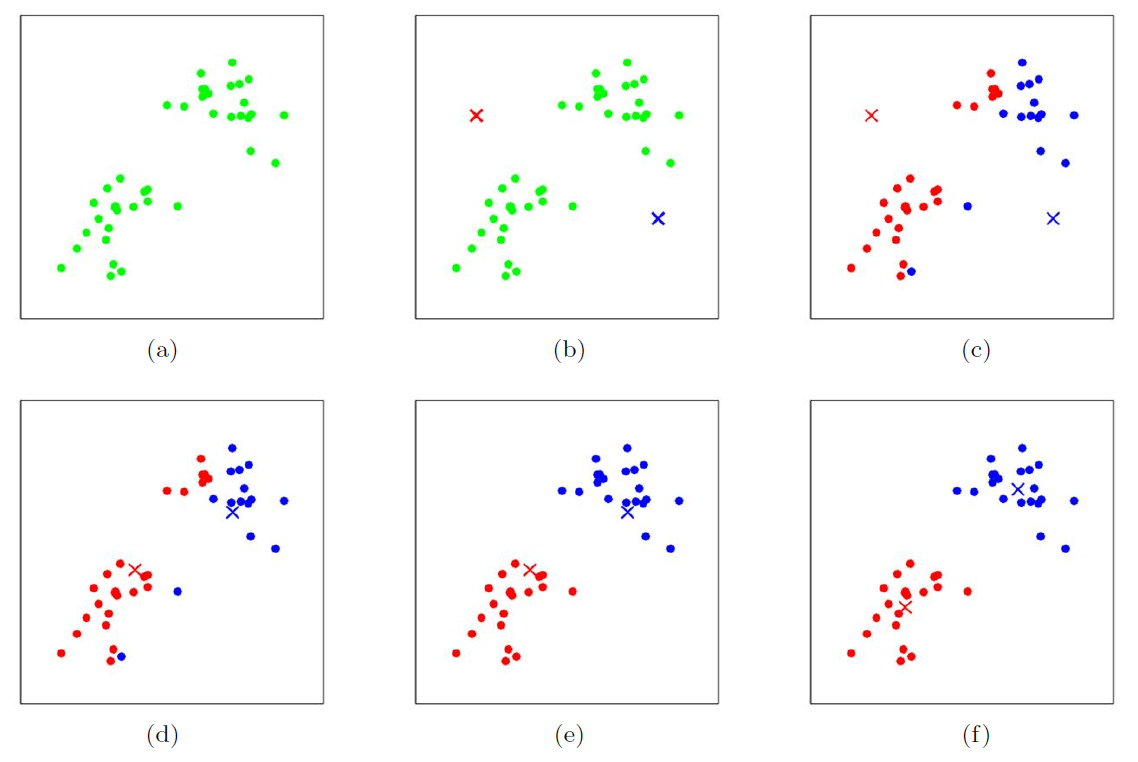
\includegraphics[width=0.7\textwidth]{kMeansClustering.png} % requires the graphicx package
   \caption{k-means聚类分析过程:“×”形代表聚类中心。}
   \label{fig:kmeans}
\end{figure}

可以发现,k-means算法的计算量相当大:每一次更新过程都要重新计算每一个样本点到聚类中心的距离。如果数据集容量较大,或者是数据集本身在持续更新(实时系统),采用上述的k-means算法可能不太合适。我们可以更改更新规则,使其变为一个在线的k-means算法(Online k-means Clustering Algorithm):

\begin{enumerate}
\item 在数据空间S中,随机生成k个聚类中心位点,其代表k个聚类;
\item 读入一个观测数据,称为$in_j$,寻找距离其最近的聚类中心,将其分配到该“获胜”的聚类中:
\begin{equation}
i \leftarrow arg\;min_i ||in_j - \mu_i||
\end{equation}
\item 通过输入的观测数据$in_j$,来更新“获胜”的聚类中心位置$mu_i$。
\begin{equation}
\mu_i \leftarrow \mu_i + \eta(in_j - \mu_i)
\end{equation}
其中$\eta$是人为调整的一个学习速率。
\item 重复之前两步,直到某一个满足终止规则为止。
\end{enumerate}

这种方法又称为“Winner-Take-All”聚类方法,因为每一次只有一个最近的聚类被更新。学习速率$\eta$的规定也将相当重要。如果$\eta$一直保持一个常数,那么这种聚类算法将不会收敛(这对于某些实时更新的系统是必要的);如果$\eta$按照某个规律衰减,那么后输入的数据对于聚类产生的影响将逐渐变小,可能导致聚类规则不准确。

另一种聚类方法的扩展称为“结构性聚类”(hierachical clustering)。这种方法基于“聚类具有子聚类”的思想。 在一种具体的结构性聚类方法(Agglomerative Hierarchical Clustering)里面,\cite{Duda2001Pattern}
每一个数据点$x_i$一开始都代表一种聚类$D_i$。算法不断地结合相隔最近的两个聚类,直到聚类总数减少到k为止。

我们后面讨论的深度空时学习网络采用了“在线聚类方法”作为神经节点的更新规则;同时也借鉴了“结构性聚类”方法的“聚类具有结构性”的思想。

\subsubsection{Gaussian混合聚类模型}
我们分析k-means聚类的统计学实质可以知道:

上述的k-means方法的损失函数$\sum^k_{i=1} \sum_{x_j\in D_i} ||x_j - \mu_i||^2$是基于独立的Gaussian聚类的:就是说,我们是假设存在数据空间$S$中存在k个独立的Gaussian分布$\{\mu_i, \Sigma_i\}$,假设每个数据$x_j$\textbf{只属于其中的一个Gaussian聚类},通过极大似然的方法用数据集$\{x_j\}$反推独立的Gaussian分布$\{\mu_i, \Sigma_i\}$的参数的过程。

然而对于不同聚类交叠较为严重的问题,k-means的处理方法并不是非常合适。
\begin{figure}[htbp]
   \centering
   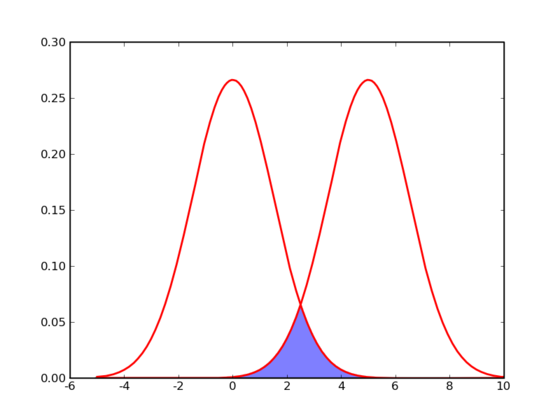
\includegraphics[width=0.5\textwidth]{kMeansProblem.png} % requires the graphicx package
   \caption{k-means聚类之难:交叠处(x=2.5)到底属于哪一个聚类?}
   \label{fig:kmeansproblem}
\end{figure}

如图\ref{fig:kmeansproblem},当我们分析x=2.5处的数据点属于哪一个聚类时,很难一刀切地通过微小的离聚类中心距离$||x_j - \mu_i||$的差距来断定聚类属性。

这时候我们产生了另一种模型,称为Gaussian混合聚类模型,其模型假设如下:

数据空间$S$中存在k个Gaussian分布的聚类$\{\mu_i, \Sigma_i\}_{i = 1\sim k}$;
空间中每一个点$x$存在一定概率属于其中每一个聚类,概率分别为$\{w_i\}$,其构成一个概率向量$\mathbf{w}$; 这样的概率向量在数据空间$S$中为一个连续的函数$\mathbf{w}(x)$。

在给定聚类属性$\{\mu_i, \Sigma_i\}_{i = 1\sim k}$和聚类概率分布$\mathbf{w}(x)$的情况下在x处观测到数据的似然概率为:

\begin{equation}
p(x|\{\mu_i, \Sigma_i, w_i \}) = \sum^k_{i=1} w_i g(x|\mu_i, \Sigma_i)
\end{equation}

其中$g(x|\mu_i, \Sigma_i)$为x单独在第i个Gaussian分布中被观测到的概率。

我们将Gaussian聚类属性参数和概率分布合并表示,称为模型假设:
$$\lambda_i(x) = \{\mu_i, \Sigma_i, w_i(x)\}, \; \lambda = {\lambda_i}$$

那么我们可以反推出在模型假设$\lambda$下,观测到数据集$\{x_j\}$的概率:

\begin{equation}
p(\{x_j\}|\lambda) = \prod^m_{j=1} p(x_j|\lambda)
\end{equation}

至此,我们可以通过极大似然概率来反解$\lambda = \{\mathbf{w}, \mathbf{\mu}, \Sigma \}$

我们假设样本点彼此相互独立,那么数据\uline{不存在协方差},高斯分布$\Sigma_i$项中不含非对角项。

为了让极大似然概率达到最大,我们可以采用一种期望值最大化算法(Expectation Maximization Algorithm),通过重复地迭代以下过程,我们可以获得需要的参数$\lambda$:
\begin{equation}
\left\{
\begin{aligned}
w_i & = & \dfrac{1}{m} \sum^m_{j=1} P(i|x_j, \lambda)\\
\mu_i & = & \dfrac{\sum^m_{j=1} [P(i|x_j, \lambda)]\, x_j}{\sum^m_{j=1} P(i|x_j, \lambda)} \\
\sigma^2_i & = & \dfrac{\sum^m_{j=1} [P(i|x_j, \lambda)]\, x_j^2}{\sum^m_{j=1} P(i|x_j, \lambda)} - \mu^2_i
\end{aligned}
\right.
\end{equation}

\begin{equation}
P(i|x_j, \lambda) = \dfrac{w_i g(x_j|\mu_i, \Sigma_i)}{\sum^k_t w_i g(x_j|\mu_i, \Sigma_i)} 
\end{equation}

我们的算法(DeSTIN)同样借鉴了混合聚类的思想:每一个数据点并不是确定性地属于一个聚类,其具有属于每一聚类的概率。

\subsubsection{自编码神经网络}

以上我们讨论了两种典型的聚类方法。接下来我们讨论另一种常见的非监督学习问题:主元分析(Principal Component Analysis)。 

主元分析的目标是:通过原始数据变量的线性组合,构造一组新的变量;这组新变量之间互相不相关,并且尽可能地做到了信号压缩:用尽可能少的变量表示所有的信息。

\begin{figure}[htbp]
   \centering
   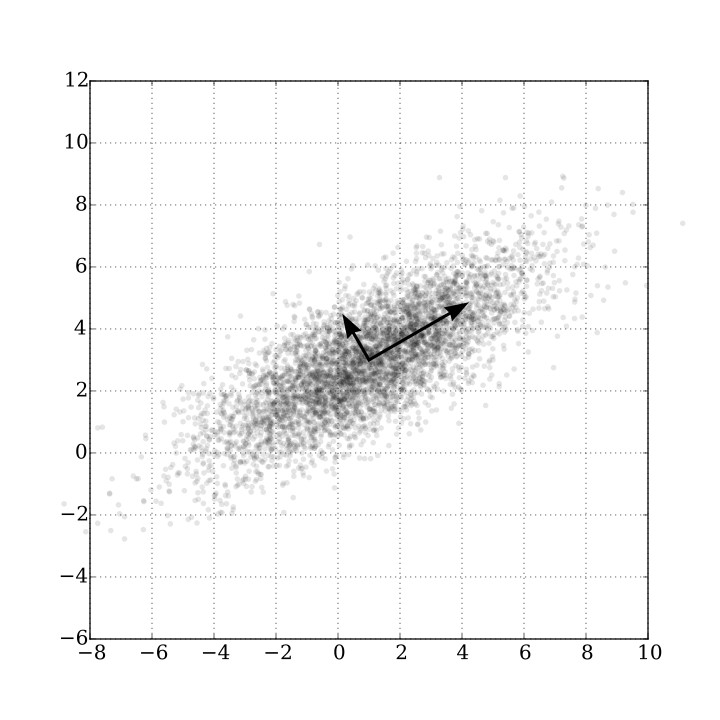
\includegraphics[width=0.5\textwidth]{PCAGaussian.png} % requires the graphicx package
   \caption{主元分析对于Gaussian分布数据的影响}
   \label{fig:pca}
\end{figure}

如图\ref{fig:pca},在原坐标下,一组二变量Gaussian分布的数据有较强的坐标相关性;通过主元分析,我们找到了一组新的坐标,在该坐标下,Gaussian分布被对角化了,并且信息集中在了一根坐标轴上。

常用的进行主元分析的方法是\uline{奇异值分解}。我们假设数据集为:$\hat{X} = [x^{(1)}; x^{(2)};...; x^{(m)}]$,对其进行奇异值分解后的结果是:

$$\hat{X} = USV^T$$

设$T_D = US$,我们假设将原坐标$\{\hat{a}\}$映射到主元的新坐标$\{\hat{b}\}$的变换矩阵为$T_L$,那么$T_L$即为$T_D$的前L列。

有趣并且有启发性的是,我们可以通过一种简单的神经网络结构获得相似的结果,其称为自编码神经网络(Auto-encoders)。

为了解决非监督学习没有训练标签的问题,我们不妨\uline{让数据本身作为标签}。

\begin{figure}[htbp]
   \centering
   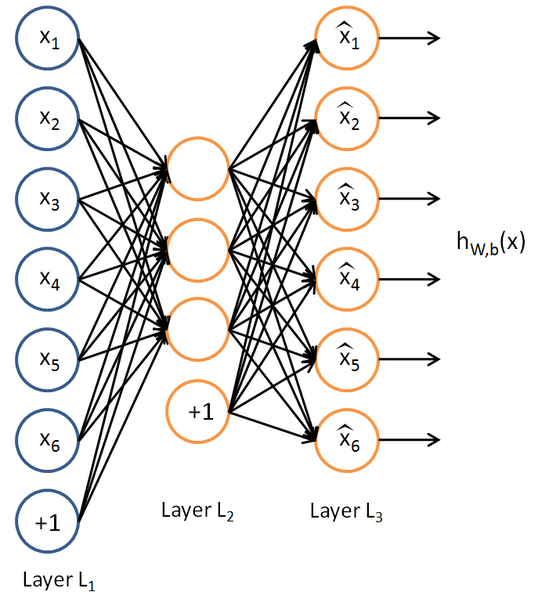
\includegraphics[width=0.5\textwidth]{Autoencoder.png} % requires the graphicx package
   \caption{自编码神经网络结构示意}
   \label{fig:pca}
\end{figure}

自编码神经网络尝试学习$h_w(x)\approx x$的函数,这件事情看上去不太有意义,但是当我们将中间层神经元数目减少时,我们可以驱使神经网络去学习数据的\textbf{压缩表示}。 

自编码神经网络的学习训练方法同上一节监督学习中的神经网络一致,而其隐藏层的神经单元往往隐含了主元分析类似的有效信息结果。

\section{深度学习}
以上我们对机器学习代表性的思想和方法进行了一个回顾, 接下来我们对机器学习的一个分支--深度学习做一个基本的介绍。

%为什么需要深度学习呢?我们已经在第一章\ref{chapter_introduction}进行过一些说明。

深度学习的背景是人工智能的发展。我们希望通过机器学习的方法构建起一个\uline{智能系统},而智能系统的基础就是\uline{其能够利用有限的资源有效地解决大量特征、高维度数据下的机器学习问题}。而传统方法下,为了处理过于复杂的问题,我们总是对数据做很多预处理,通过先验知识将问题化归到小特征空间上去,这样的方法过于困难,并且缺乏通用性。\cite{Duda2001Pattern}

深度学习的目的就在于突破学习算法的“维度困境”\cite{bellman1957dynamic},通过多层网络结构来实现高维度信息的处理。

从结构上来说,深度学习结构定义为一个包含多层非线性变换的模型。\cite{bengio2009learning}除数据的输入层外,每一层的输入信号都由前面一层的输出产生;通过一些监督、非监督学习的学习方法,输出数据给下一层结构。

从功能上来说,深度学习尝试从未经人为处理的现实的高维度数据中直接进行特征学习。比如,在没有给机器任何的先验信息的前提下,给出大量的真实照片,让机器自己去提取照片里面的物体、进行边缘检测等等。

深度学习的核心部分在于\uline{如何从海量的数据里面提取有效特征},即特征提取。每一层提取到的特征随着层数变深逐渐全局化。最终我们可以利用不同层的提取的特征进行后期的监督学习(回归、分类)或者非监督学习(聚类、主元分析)。

深度学习起源于神经网络的研究。普通的神经网络只包含了一层隐藏层,当我们将隐藏层拓展为多层时,就成为了“深度神经网络(Deep Neural Network)”。研究发现\cite{bengio2009learning},深度神经网络具有较普通神经网络更加好的非线性特征提取能力。然而,深度神经网络的问题在于:
\begin{enumerate}
\item 过拟合现象: 由于神经网络的参数过多,数据量不够导致过拟合容易发生;
\item 局部极值问题: 使用监督学习方法训练深度网络时,求解的损失函数往往是高度非凸的优化问题,存在各种局部极小值点,使得梯度下降类的方法效果不好;
\item 梯度弥散问题: 梯度下降法的另一个问题是,随着网络深度增加,反向传播的梯度值会急剧减小,以至于最初的几层神经网络无法进行有效的学习;
\item 训练过程非常耗时,消耗计算资源;算法效率低。
\end{enumerate}

为了解决过拟合的问题,陆续有很多正则化的方法提出;一个更加有效的方法是,“随机剔除(dropout)”方法\cite{JMLR:v15:srivastava14a},即在训练的过程中随机地关闭掉一些隐藏层的神经元,以防止整个系统产生一些特定的对于神经元的依赖关系。另外一个解决过拟合的方面是,我们需要获取足够多的样本:足量的数据能够保证过拟合现象不会发生。

而为了解决局部极值、梯度弥散两个问题,学界诞生了一种“逐层贪婪训练”的方法:每一次只训练一层网络,当这一层网络训练结束以后,固定之前训练的所有k-1层网络(不再训练),增加第k层在网络的最后进行学习(通常用自编码器进行无监督学习);各层单独训练后的权重当做整体训练的初始值,然后对整个网络进行监督训练,获得“微调”效果。具体过程参见\cite{deep_learning_ufldl}。


最后,为了更有效地提取特征,提高算法效率,两种重要的基于以上思路的改进产生了的新的深度学习算法:\uline{卷积神经网络}\cite{hinton2006fast}与\uline{深度信度网络}\cite{lee2009convolutional}。这两种算法的产生标志着深度学习方法的成熟化。本节接下来简要介绍这两种深度学习算法。

\subsection{卷积神经网络}
卷积神经网络(Convolutional Neural Network,CNN)在处理2D图像的问题上取得了成功。我们主要围绕其在图像处理上基于深度神经网络进行的改进进行说明。

\subsubsection{部分联通网络的必要性}
我们已经知道传统“深度神经网络”(DNN)面临的最终困难:“全连接”的神经网络非常消耗计算资源和时间:我们以一层隐藏层的神经网络为例:

当输入数据维度为n,标签维度为k时,第一层神经元个数为n个,第二层假设为$\sqrt{nk}$个,第三层为k个;那么其需要的总权重参数数目为:

$N(\mathbf{w}) = (n+1)\cdot\sqrt{nk} + (\sqrt{nk}+1)\cdot k \propto n\sqrt{n}$

假如我们的输入数据为手机屏幕图片,其维度量级大致为100*100像素点;假设你要学习图像的100个特征,那么我们需要的参数$N(\mathbf{w})$量级大概是:$100*100*\sqrt{100*100*100} = 10^7$。

对于高维度数据,全连接(指每一层所有神经元与其相邻一层所有神经元相连接)神经网络不符合现实。我们应当采用\textbf{部分联通网络}的结构:\uline{每一个神经网络仅连接输入单元的一部分},对于图片来说,可能是相邻区域。

\begin{figure}[htbp]
   \centering
   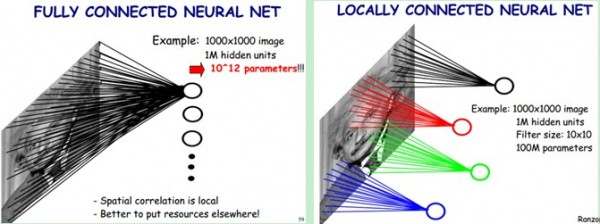
\includegraphics[width=0.7\textwidth]{LocallyConnectedNetwork.jpg} % requires the graphicx package
   \caption{部分连接网络示意}
   \label{fig:localnetwork}
\end{figure}

网络部分联通(locally connectivity)的思想,也是受启发于生物学里面的视觉系统:视觉皮层的特定神经元只由相应某些特定视网膜区域才能刺激。

仍然是100*100的像素点输入层,假如第二层的神经元只和附近的10*10个像素点相连,那么权重值的数目降到了原来的百分之一。假定原来第二层有100个神经元,原权重值数目为:$100*100*100 = 10^6$;现权重值数目为$10*10*100 = 10^4$。


\subsubsection{图像特征的全局性,参数共享与卷积}
自然图像具有一种特性:同一幅图像的某一块区域的统计特性(比如频谱大小)和其他部分基本相同。 \cite{Hyv2009Natural}这意味着如果我们在某一块小区域学习到了某一个特征,其在图像上其他的位置可能也会有所反映。

这启发我们先在一个小区域进行特征学习,再将该特征对应到整个区域上去。具体来说,我们可以在一个大尺寸图像上随机选取一个小区域(比如$8*8$的小块),通过无监督学习的方法(比如自编码器)进行了特征$\{a\}$的学习;再将该特征$\{a\}$作为一个探测器,应用到图像的任意地方去。

数学上,为了建立起某一个局部区域特征和图像其他位置的作用,我们可以进行\textbf{卷积}操作;笔者简单描述一下二维离散有限域卷积的公式。

设某一$M\times N$的图像对应一个离散$(x,y)$的函数
$f(x,y) \;(x = 1\sim M,y = 1\sim N)$,
其中某一个小区域对应的函数为
$g(x,y) \;(x = 1\sim A, y = 1\sim B)$,那么两个函数卷积的结果是:
$$f*g(x,y) = \sum^{A-1}_{p=0} \sum^{B-1}_{q=0} f(p,q)g(x-p,y-q) \,\; x = 1\sim M-A+1, \,y = 1\sim N-B+1$$

直观的理解,就是将小区域水平、垂直翻转,再与大单元的相应位置单元的值相乘,最后进行求和。如图\ref{fig:conv}所示。我们将对大区域进行卷积的小区域称为\textbf{卷积核}。

\begin{figure}[htbp]
   \centering
   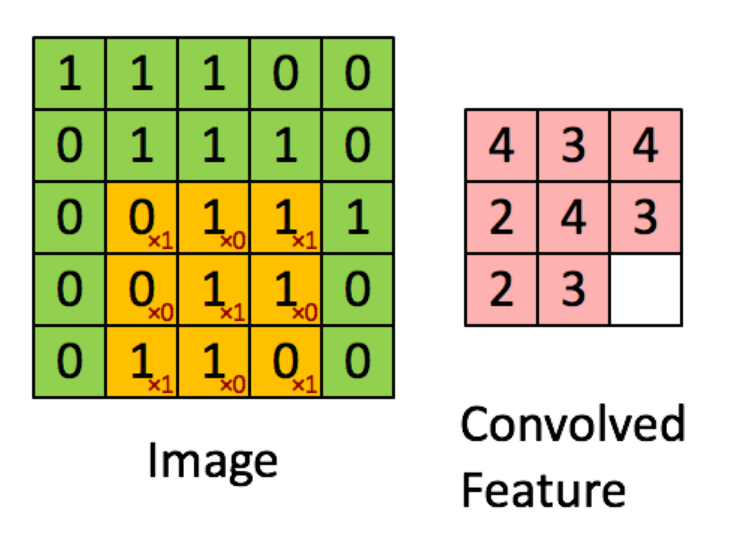
\includegraphics[width=0.6\textwidth]{Convolution.png} % requires the graphicx package
   \caption{二维离散有限卷积示意}
   \label{fig:conv}
\end{figure}

在此我们要\textbf{拓宽卷积的语义}。在以上过程中,卷积核表示图像的一部分区域$g(x,y)$,卷积操作的运算为$\sum g(x-p,y-q)\cdot f(p,q)$,如果我们将卷积核的值看作系数,则有卷积操作变为:
\begin{equation}
Conv(f(x,y))  = \sum_{i,j} w(x-i,y-j)\cdot f(i,j)
\end{equation}

此时卷积已经变为了一种某个区域内(大小为$A\times B$)的元素线性变换再加和的过程。
广义的卷积,就是一个线性变换再求和的过程;此时的\uline{卷积核不再理解为图像的一个区域,而是理解成\textbf{线性变换的系数$w_{i,j}$和尺度}}。

卷积相当于是一种全局的线性算子,其平移并作用于整个图像,进行线性运算并加和,输出特征的卷积结果。

我们将卷积的过程看作一种特殊的神经网络层间过渡过程:假设输入层的数据为$x$,那么卷积层的神经元表示为:
\begin{equation}
\label{eqn:conv}
a^l_{i,j} = g(z^l_{i,j}) = g((w^l \ast x)_{i,j} + b_l)
\end{equation}

其中,$g(z)$为Sigmoid激活函数,$a^l$为卷积层的神经元激活值,$\mathbf{w^l}$作为卷积核充当了之前连接两层神经元的权重值的功能(也将是训练的核心)。$b_l$为常数偏移值,之前都合并在$\mathbf{w^l}$中,在2D模型中为了表示方便,将其提出。

\begin{figure}[htbp]
   \centering
   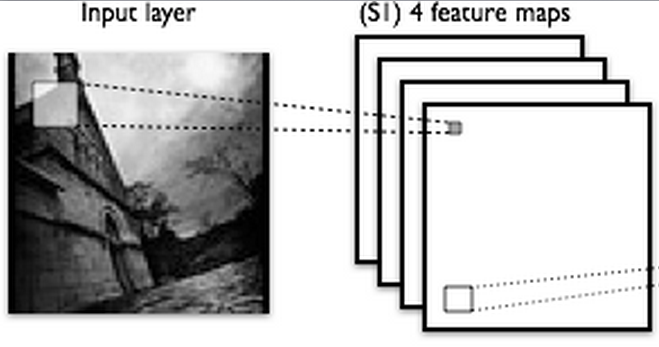
\includegraphics[width=0.6\textwidth]{ConvolutionKernal.png} % requires the graphicx package
   \caption{通过卷积进行输入层到中间层的连接}
   \label{fig:convker}
\end{figure}

%举一个具体的例子描述卷积通道的形成的过程:假设我们有一副$96\times96$的图像,我们选取了一个$8\times8$的区域作为其卷积核:
%\begin{enumerate}
%\item 我们对该$8\times8$的样本区域进行自编码学习,假设其隐含单元数为100;
%\item 学习完成后,我们将抽取的$8\times8$区域同整个图像进行卷积运算
%\end{enumerate}

值得一提的是,我们可以采用自编码器作为卷积核,进行卷积层的相关操作,参见\cite{deep_learning_ufldl}。

对于一幅高维度图像,我们当然不会只提取一个特征。 对于多个特征的情况,我们可以设置多个卷积核,每个卷积核根据\ref{eqn:conv}计算得到一个\uline{卷积通道}(也称为特征图(feature map));最终生成的卷积层成为一个多层的三维结构。可以发现,当前后两层结构都为三维结构时,联系这两层结构的权重值$w^{lk}_{i,j}$将成为四阶张量。

\subsubsection{特征归并:池化}
我们通过卷积核构造出了卷积层,并希望能够进行下一层神经网络的搭建。然而我们面临着计算量的困境:直接卷积得到的卷积层神经元过多。

对于一副$96\times96$的图像,假设我们训练了400个$8\times8$的卷积核,那么每一个卷积核将产生$89^2=7921$维的卷积通道;卷积层的总维度将高达:$89^2*400 = 3168400$。

以下我们介绍对特征进行归并化简的方法:池化(pooling)。池化的操作非常简单:\uline{将每个卷积通道划分为可数的区域,计算每个区域特征的平均值(或最大值)},并将其作为池化后的神经元结果。

池化的合理性在于卷积的平坦性:某一个位置的卷积结果与其相邻位置卷积结果不会相差很多;基于此我们就可以对于图像某个区域进行归并统计。

以上我们介绍了卷积神经网络的主要思想,其训练过程同普通神经网络一样,也采用反向传播算法。由于其提取图像特征的有效性,通常层数比相同效果的深度神经网络要少得多,因而训练将更为迅速。

图\ref{fig:lenet}是一个典型的卷积神经网络(CNN)的结构,其基本构造为:输入的图像先进行卷积核特征提取,再池化;再进行卷积核特征提取,再池化;最后输出到全连接的神经网络中进行监督训练。

\begin{figure}[htbp]
   \centering
   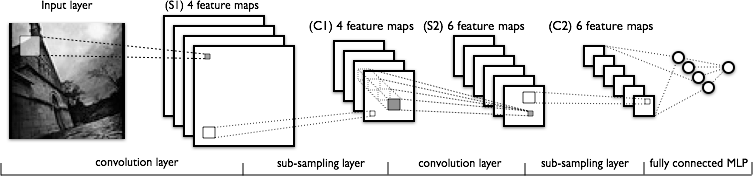
\includegraphics[width=0.8\textwidth]{Lenet.png} % requires the graphicx package
   \caption{典型的卷积神经网络结构(LeNet)}
   \label{fig:lenet}
\end{figure}

\subsection{深度信念网络}
同CNN不同,深度信念网络(Deep Belief Networks, DBNs)是一种直接基于Bayes概率的方法,和原来的神经网络方法有较大的不同。

\subsubsection{受限Boltzmann机模型}
在介绍DBN之前,我们先要介绍构成DBN的基本单元——受限Boltzmann机(Restricted Boltzmann Machine, RBM)。该模型是用于判断数据的属于不同类别的概率的(即分类模型),其优势在于训练较为简单,便于在DBN网络中使用。

\begin{figure}[htbp]
   \centering
   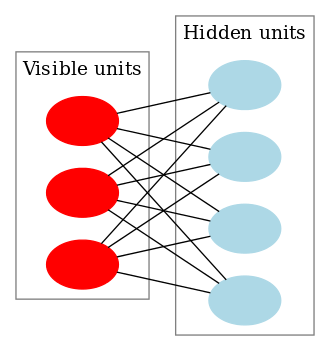
\includegraphics[width=0.4\textwidth]{RestrictedBoltzmannMachine.png} % requires the graphicx package
   \caption{受限Boltzmann机示意}
   \label{fig:rbm}
\end{figure}

如图\ref{fig:rbm},RBM由可见层$\{v_i\}$和隐藏层$\{h_j\}$,可见层的常数偏置单元$\{a_i\}$以及隐藏层的常数偏置单元$\{b_i\}$组成。其中$\{v_i\}$,$\{h_j\}$的值在标准的RBM中只能取0或1。类似于神经网络,我们定义单元之间的连接权重$\mathbf{w} = (w_{i,j})$。

我们定义这个结构的\textbf{能量}为:
\begin{equation}
E(v,h) = - \sum_i a_i v_i - \sum_j b_j h_j - \sum_i\sum_j v_i w_{i,j} h_j
\end{equation}
或者简记为:
$$E(v,h) = -a^T v -b^T h - v^T \mathbf{w} h$$

在这个网络中,$v,h$的联合概率分布可以表示为:
\begin{equation}
P(v,h) = \dfrac{1}{Z} e^{-E(v,h)}
\end{equation}

其中Z为配分函数,即所有$(v,h)$可能取值下$e^{-E(v,h)}$的加和,即归一化系数。

那么容易求得$v$的边缘分布函数为:
\begin{equation}
P(v) = \dfrac{1}{Z} \sum_h e^{-E(v,h)}
\end{equation}

可以发现,RBM是一个双向对称结构;在给定$v$的情况下,$h$的激活情况相互独立;反之亦然。我们可以得到以下条件概率公式:

\begin{equation}
P(v|h) = \prod^m_{i=1} P(v_i|h)\;,\; P(h|v) = \prod^n_{j=1} P(h_j|v)
\end{equation}

每一个单元激活概率由Sigmoid函数g(z)给出:

\begin{equation}
P(v_i=1|h) = g(a_i + \sum^n_{j=1} w_{i,j}h_j )\;,\; P(h_j =1|v) = g(a_i + \sum^m_{i=1} w_{i,j}v_i )
\end{equation}

RBM有着较为简单的训练方法:假设输入训练集为$V = [v^{(1)};v^{(2)};...;v^{(m)}]$ ,RBM的训练目标为使得v的产生概率最大;

\begin{equation}
arg\; max_{\mathbf{w}} \prod_{v\in V} P(v)
\end{equation}

或者等效于:

\begin{equation}
arg\; max_{\mathbf{w}} \sum_{v\in V} log P(v)
\end{equation}

我们仍然可以采用梯度下降法对其进行训练,在此不赘述。

\subsubsection{DBN的结构}

如图\ref{fig:dbn}我们将RBM进行层级堆叠,并且采用“逐层贪心训练”的方法,就可以实现所谓DBN的架构。\cite{hinton2006fast}

\begin{figure}[htbp]
   \centering
   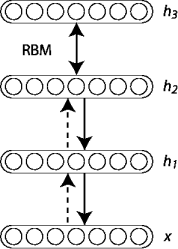
\includegraphics[width=0.4\textwidth]{DeepBeliefNetwork.png} % requires the graphicx package
   \caption{DBN架构示意}
   \label{fig:dbn}
\end{figure}

我们分析DBN能够提取出训练数据层次结构特征的原因:在DBN模型中,观测变量$x$与前$l$层隐藏变量$h^1,h^2,..h^l$的联合概率分布如下:(由RBM模型可推知)

\begin{equation}
P(x,h^1,h^2,...,h^l) = (\prod^{l-2}_{k=0} P(h^k|h^{k+1})) P(h^{l-1},h^l)
\end{equation}

其中$x=h^0$,$P(h^{k-1}|h^k)$反映出第k层RBM的由隐藏层到可见层的条件概率,$P(h^{l-1},h^l)$为第l层RBM的可见层与隐藏层的联合概率。

可见上式构成一个良好的递推结构,那么我们可以从一层RBM训练出发;将底层的隐藏层信息作为上一层的可见层输入,固定底下的层数训练最高的一层;训练完所有层数后再使用监督学习方法进行全局微调,即完成了整个DBN训练过程。

由于DBN大部分内容与本论文无关,此处不展开介绍,详见\cite{lee2009convolutional}。
\chapter{DeSTIN算法的介绍与测试}\label{chapter_algorithm}
\graphicspath{{chapter3/figure/}}

本章我们将对我们研究的深度空时关系推断网络(Deep SpatioTemporal Inference Network,DeSTIN)进行介绍;并且基于此进行测试,分析其算法的可靠性以及移植到硬件上的可能性。

\section{DeSTIN算法介绍}

上一章笔者介绍了一些常见的深度学习方法。这些方法在应对“维度困境”,在高维度数据处理和特征提取上产生了不错的成果。但是这些算法应用的方面有一定的局限性:这些方法都以处理静态问题为主,不能很好地处理包含时间序列的问题。虽然在深度神经网络(DNN)的基础上发展出了一种循环神经网络(Recurrent Neural Network,RNN)的方法,但是其具有DNN方法与生俱来的缺陷:全连接网络,计算效率较差;很深的反向传播距离使得其训练较为困难。

我们将首先从概率论的角度进行时间序列问题解决方案的描述,再进一步落实到我们使用的DeSTIN算法上来。随后我们将对DeSTIN算法做一些数据集测试,检验其学习能力以及缺陷。

\subsection{DeSTIN算法的理论基础}

本节的理论分析主要基于DeSTIN的第一篇论文。\cite{Arel2009DeSTIN}

我们考虑\uline{在一个深层神经网络结构里,为了准确反映时间序列关系,一个神经节点应当如何进行其信度状态更新}的问题。

我们首先做一个假设:\uline{被观测的数据的序列结构能够被结构化地表示出来;于此同时,序列里两件事的长程相关性不会和这两件事的间隔准确地相关}。

这个假设让我们对数据的结构有一个先验的判断:其结构能够被多层的网络状态抽象提取出来。于此同时,由于数据的长程相关性不与间隔严格相关,我们可以采用一个相对粗糙时序度量。

我们主要讨论\uline{一个神经网络节点下一时刻的信度状态如何由当前自身的信度状态、母节点的信度状态和当前的观测值来确定}。整个神经网络接收一个外界输入的序列集,并尝试从序列集中提取特征规律,通过自身的信度状态表达出来。

现对后续讨论的符号进行规定:假设我们讨论的节点在当前时刻的信度状态为$b(s)$,其中s指\uline{输入节点的任何可能的状态序列},S指整个状态序列的空间(序列集);此节点存在母节点,其信度状态为$c$;此节点下一个时刻的信度状态为$b^\prime(s^\prime)$;当前观测值记为$o$。

由信度状态的定义以及以上假设知:
\begin{equation}
b^\prime(s^\prime) = Pr(s^\prime|o,b,c) = \dfrac{Pr(s^\prime, o, b, c)}{Pr(o, b, c)}
\end{equation}

由条件概率公式,上式可以化为:
\begin{equation}
b^\prime(s^\prime) = \dfrac{Pr(o|s^\prime,b,c)Pr(s^\prime|b,c)Pr(b,c)}{Pr(o|b,c)Pr(b,c)}
\end{equation}

我们再假设:\uline{观测值不依赖于节点的信度状态b、c,只依赖于输入的序列状态$s$、$s^\prime$},那么$Pr(o|s^\prime,b,c) = Pr(o|s^\prime)$,上式进一步简化为:

\begin{equation}
b^\prime(s^\prime) = \dfrac{Pr(o|s^\prime)Pr(s^\prime|b,c)}{Pr(o|b,c)}
\end{equation}

此处$Pr(s^\prime|b,c) = \sum_{s\in S} Pr(s^\prime|s,c) b(s)$,进一步改写上式:

\begin{equation}
\label{eqn:destin}
b^\prime(s^\prime) = \dfrac{Pr(o|s^\prime)\sum_{s\in S} Pr(s^\prime|s,c) b(s)}{\sum_{s^{\prime\prime}\in S}Pr(o|s^{\prime\prime})\sum_{s\in S} Pr(s^{\prime\prime}|s,c) b(s)}
\end{equation}

此时分母为归一化因子。我们考虑公式\ref{eqn:destin}中分子每一项的意义。$Pr(o|s^\prime)$反映出模式静态的相似度(当前的观测值与之后输入序列的关系);而$Pr(s^\prime|s,c)$\uline{反映系统演化过程}(当前输入序列,母节点信度与之后输入序列的关系)。在我们的结构中,母节点的信度状态$c$通过以下方式进行选择:

\begin{equation}
c = arg\;max_s b_p(s)
\end{equation}

其中$b_p(s)$为母节点的信度关于输入状态的分布。即我们取使母节点信度最大的输入状态$s$作为$c$。

我们重新考察式\ref{eqn:destin},可知:如果我们能够较好地获得$Pr(o|s^\prime)$和$Pr(s^\prime|s,c)$的表示,就可以由当前信度状态和观测推知下一个时刻的信度状态,即进行了序列特征的识别。

文章\cite{Arel2009DeSTIN}中基于式\ref{eqn:destin}进行了说明:$Pr(o|s^\prime)$可以通过\uline{在线聚类方法}进行学习(见第二章k-means聚类小节);而$Pr(s^\prime|s,c)$由神经网络的结构关联进行反映。

基于以上理论,我们展开DeSTIN算法的介绍。

\subsection{DeSTIN算法的整体框架}

DeSTIN构架的网络结构如图\ref{fig:destinarchi}。其借鉴了深度信念网络的想法:在层与层之间传递节点学习的信度状态(Belief State),将下面一层的四个(或者两个)相邻的子节点信度的状态合并,作为上面一层节点的输入信号。

对于每一个节点,信度状态具体体现为:节点内部进行聚类计算,判断输入的数据$o$输入分别属于其内部k个聚类的概率:${P(h_i|o)}_{i:1\sim k}$,将这一组概率称为其输出的信度状态。

\begin{figure}[htbp]
   \centering
   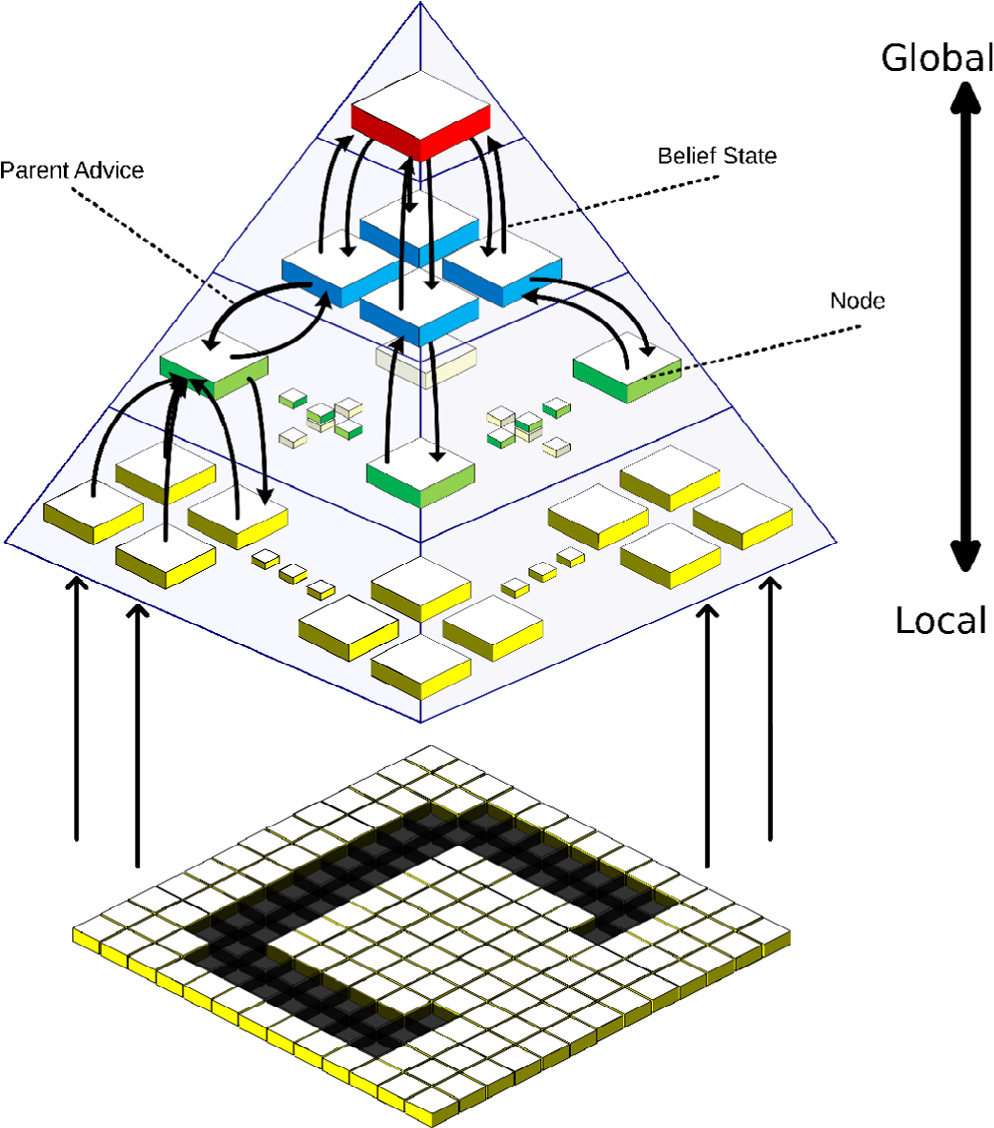
\includegraphics[width=0.5\textwidth]{DeSTINArchitecture.png} % requires the graphicx package
   \caption{DeSTIN算法的架构}
   \label{fig:destinarchi}
\end{figure}

对于整个结构,数据序列由底层逐个输入,底层神经元根据输入数据调整自身的参数,尝试获得其中较为显著的空间、时间关系,将其体现在信度状态的输出中;上一层接收到下一层的信度状态输入后,尝试捕捉\uline{更加宏观的空间时间关系},并进行自身权重调整;整个结构由下往上来看,\uline{提取的空间时间特征不断地全局化,最终每一层都产生不同层次的特征提供给后续的监督学习}。

\subsection{单个神经元的online k-means聚类算法}
以下我们详细介绍单个神经元采用的online k-means clustering算法,分析其如何进行学习、以及输出信度状态的。

根据整体DeSTIN结构的要求,一个具体的神经元应当具有如图\ref{fig:neuronstr}的结构。

\begin{figure}[htbp]
   \centering
   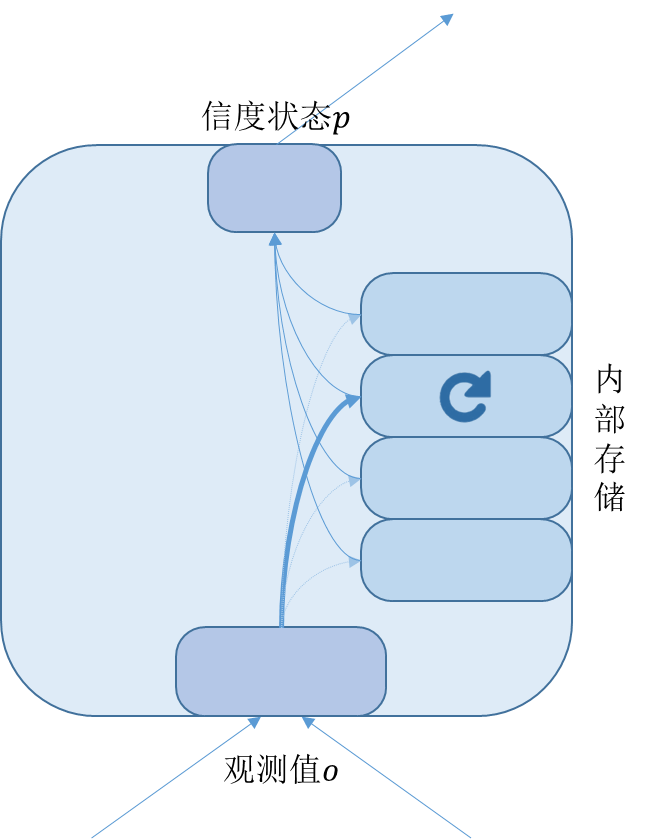
\includegraphics[width=0.4\textwidth]{NeuronStructure.png} % requires the graphicx package
   \caption{DeSTIN神经元的抽象结构}
   \label{fig:neuronstr}
\end{figure}

每一个任务周期内,神经元将按顺序执行以下步骤:
\begin{enumerate}
\item 聚类判断过程: 接收输入信号$o$(底层为数据输入,上层为下层的信度状态输入);根据自己的聚类参数判断其属于哪一个聚类;
\item 学习过程: 根据输入数据更新自身的聚类特性;
\item 信度计算过程: 根据$o$以及更新后的聚类参数计算其属于每一个聚类的概率,作为信度状态输出。
\end{enumerate}

我们将以上过程具体化。假设输入的观测值为$o$,为了可视化方便起见,假设输入数据$o$为I=2维;按照传统聚类的方法,我们初始化J个聚类(此处$J=4$),其中心为$\{\mu_j\}$,参数方差为(高斯分布)$\{\sigma^2_j\}$,注意到$\mu_j, \sigma^2_j$均为I维的向量。如图\ref{fig:onlineclus1}所示。

\begin{figure}[htbp]
   \centering
   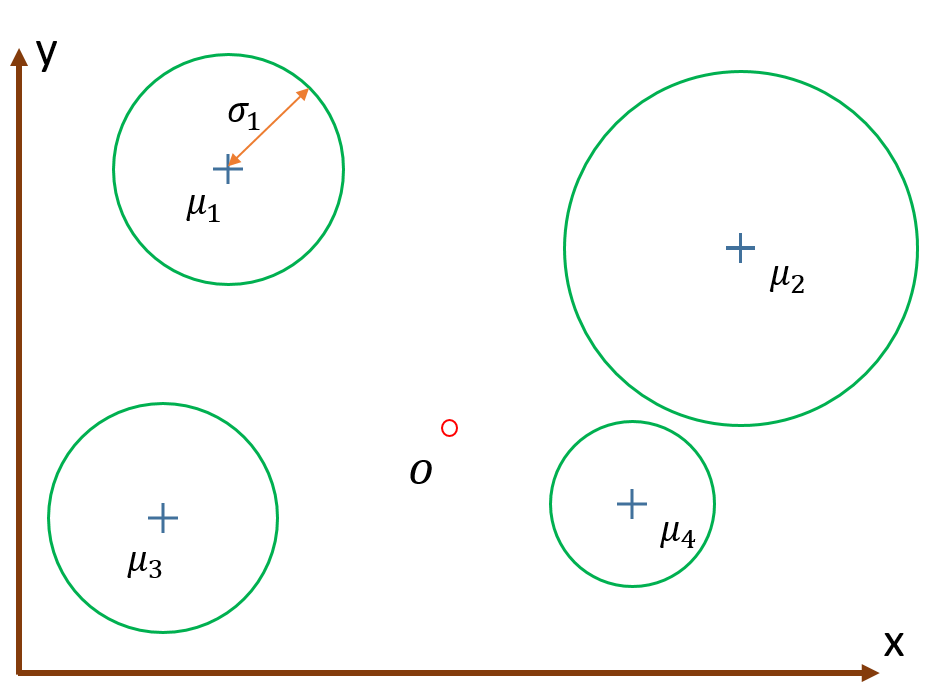
\includegraphics[width=0.5\textwidth]{OnlineClustering1.png} % requires the graphicx package
   \caption{聚类算法1:参数以及初始化}
   \label{fig:onlineclus1}
\end{figure}

首先,我们执行聚类判断过程:如图\ref{fig:onlineclus2},我们采取“赢家通吃(Winner-Takes-All)”的原则进行聚类的判断:根据欧氏距离(的平方)$d_j = ||o - \mu_j||^2$来判断聚类归属,最小者胜利,具体公式如下:
\begin{equation}
j0 = arg\;min_j d_j = arg\;min_j ||o - \mu_j||^2
\end{equation}

\begin{figure}[htbp]
   \centering
   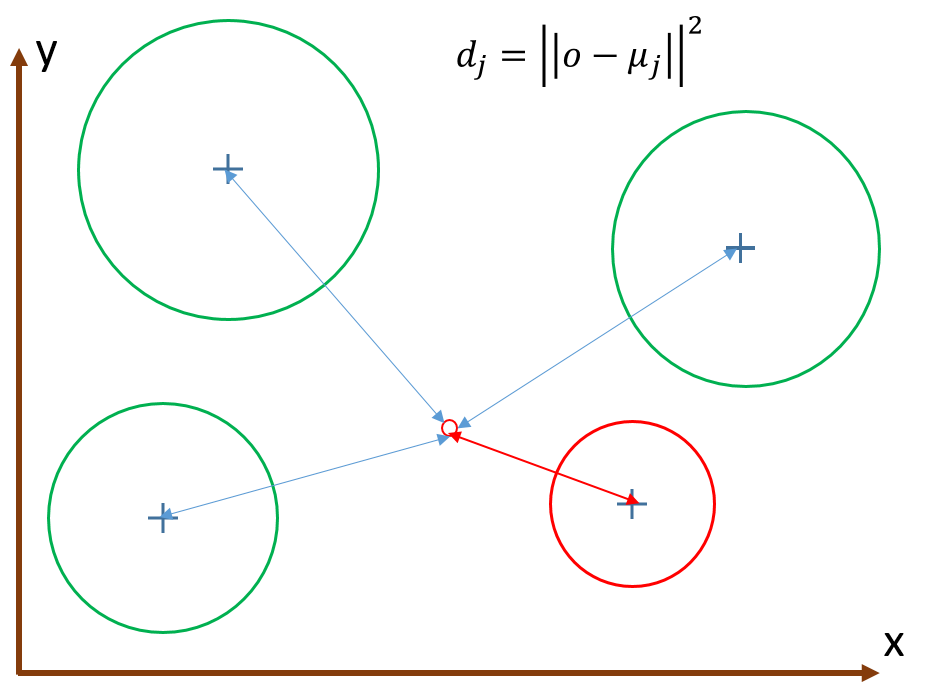
\includegraphics[width=0.5\textwidth]{OnlineClustering2.png} % requires the graphicx package
   \caption{聚类算法2:聚类判断过程}
   \label{fig:onlineclus2}
\end{figure}

然后,我们进行赢家的聚类更新:如图\ref{fig:onlineclus3},设定圆心聚类学习速率为$\alpha$,方差聚类学习速率为$\beta$,那么:
\begin{equation}
\left\{
\begin{aligned}
\mu_{j0} & \Leftarrow \mu_{j0} + \alpha (o - \mu_{j0}) \\
\sigma^2_{j0} & \Leftarrow \sigma^2_{j0} + \beta (d_{j0} - \sigma^2)  = \sigma^2_{j0} + \beta ((o-\mu_{j0})^2 - \sigma^2)
\end{aligned}
\right.
\end{equation}

\begin{figure}[htbp]
   \centering
   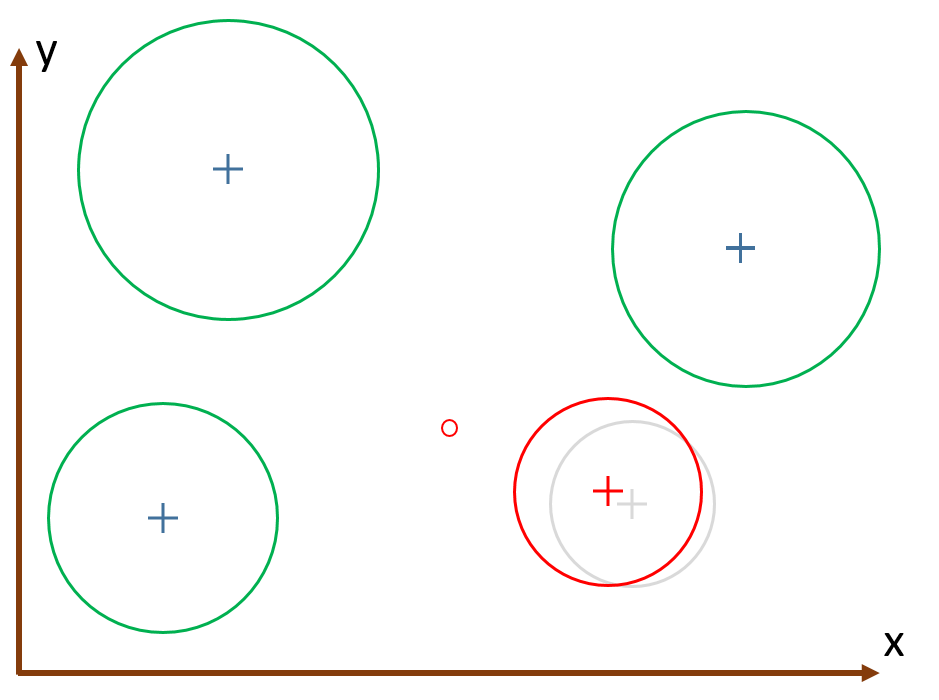
\includegraphics[width=0.5\textwidth]{OnlineClustering3.png} % requires the graphicx package
   \caption{聚类算法3:聚类学习过程}
   \label{fig:onlineclus3}
\end{figure}

最后,我们根据更新后的聚类信息进行信度状态的计算。我们借鉴了Gaussian混合模型里面概率计算的方法,但是进行了简化\cite{Young2014Hierarchical}。如图\ref{fig:onlineclus4},我们根据归一化的Euclid距离$n_j$进行概率估计:当数据点$o$与我们的聚类距离较小时,其属于聚类的概率便较大;我们假设数据的距离与其属于该聚类的概率成反比,那么有:
\begin{equation}
\begin{aligned}
n_j & = \sum_i \dfrac{||o_i-\mu_{i,j}||^2}{\sigma^2_{i,j}} \\
p_j & = \dfrac{n_j^{-1}}{\sum_{j^\prime} n_{j^\prime}^{-1}}
\end{aligned}
\end{equation}

\begin{figure}[htbp]
   \centering
   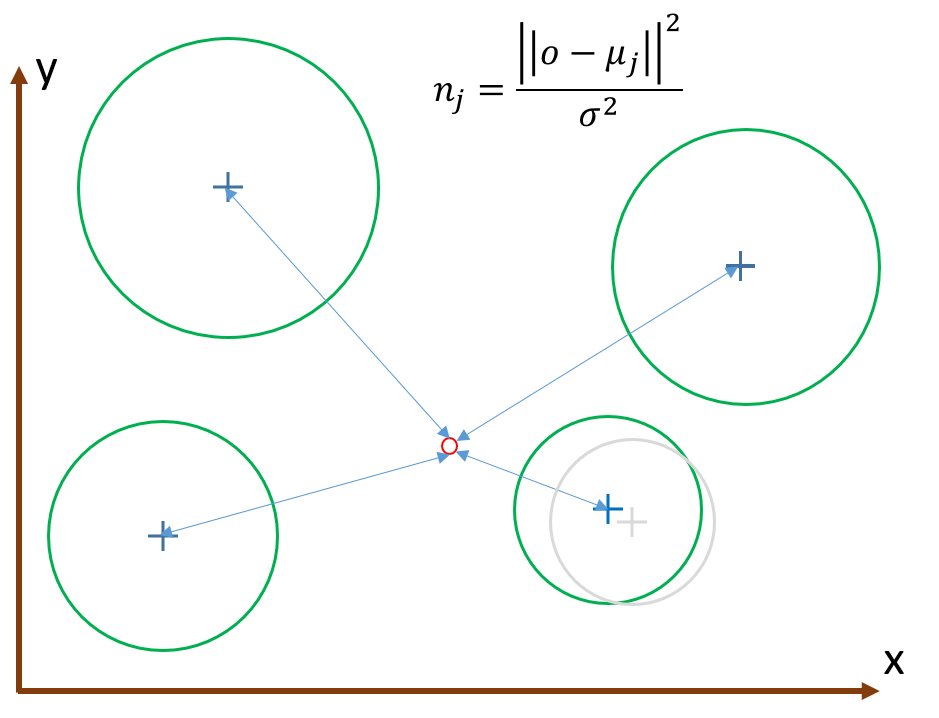
\includegraphics[width=0.5\textwidth]{OnlineClustering4.png} % requires the graphicx package
   \caption{聚类算法4:信度状态计算过程}
   \label{fig:onlineclus4}
\end{figure}

可以看出,我们的算法在传统聚类和混合聚类方法中取了一个平衡:\uline{只更新最近的一个聚类;但是考虑数据点聚类归属时,输出其属于每个聚类的概率},这样既保证计算不会过大,又能够较为准确地反映结果。

我们采用的聚类方法的主要过程介绍完了,但是为了弥补原算法的一个不足之处,我们引入\textbf{饥饿值}的概念\cite{Young2010A}。

我们可以想象一种情况:假设真实的数据有四个团簇,我们也初始化了四个聚类;但是很不幸的是,有一个聚类的初始化距离4个数据团簇都很远;那么每一次更新时该聚类都不能移动,最终这个聚类位置完全不能反映数据团簇情况,称为“\textbf{空闲类}”,而空闲类较多时,聚类数目就不足以反映真实团簇的数目:3个聚类在对应4个数据团簇时效果就没有那么理想了。

为了解决这个问题,我们为每一个聚类再增加一个“饥饿值”参数$\{\psi_j\} (\psi_j:0\sim 1)$:假设在某一个操作周期中,该聚类未被更新,其饥饿程度增大,$\psi$减小;反之$\psi$增大。
\begin{equation}
\psi_j \Leftarrow \left\{
\begin{aligned}
& \gamma \psi_j  \\
& \gamma \psi_j + (1-\gamma)
\end{aligned}
\right.
\end{equation}

其中$\gamma:0\sim1$为“饥饿参数”。这样我们可以保证$\{\psi_j\}$一直处于$0\sim 1$的范围内。如图\ref{fig:onlineclus5},在聚类判断过程中,我们将“饥饿值”也作为考虑的因素,即
\begin{equation}
j0 = arg\;min_j (\psi d_j) = arg\;min_j (\psi ||o - \mu_j||^2 )
\end{equation}

\begin{figure}[htbp]
   \centering
   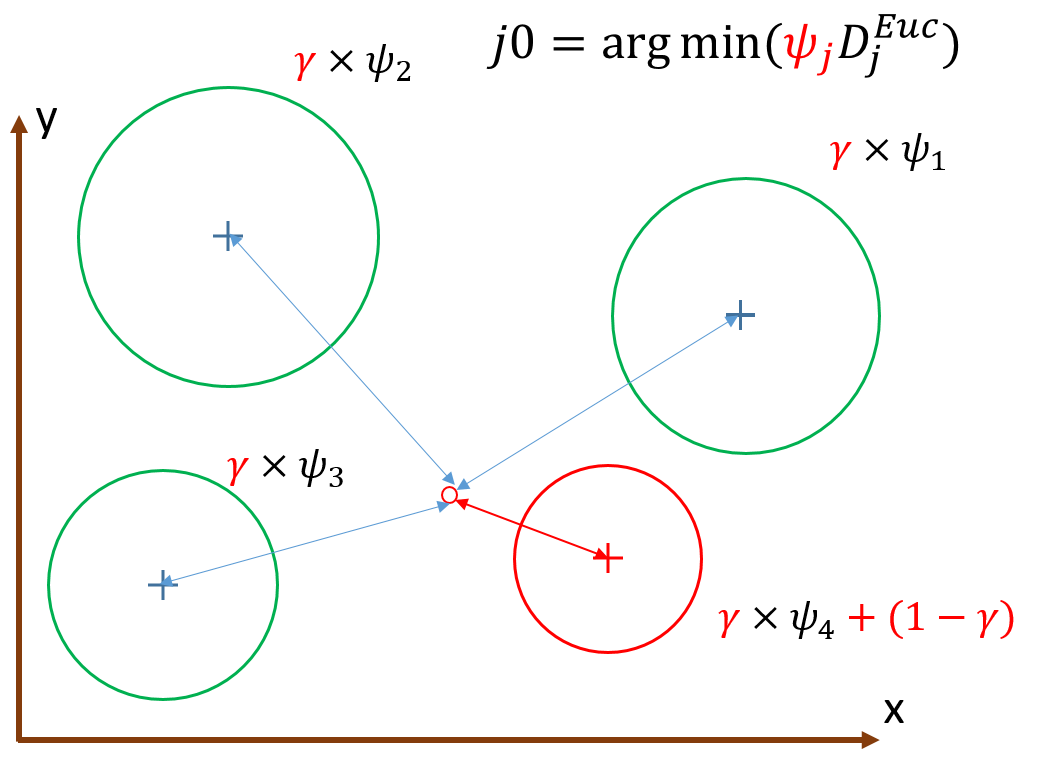
\includegraphics[width=0.5\textwidth]{OnlineClustering5.png} % requires the graphicx package
   \caption{聚类算法5:饥饿值的引入}
   \label{fig:onlineclus5}
\end{figure}

我们将在线聚类算法的过程总结为MATLAB代码如下:

\begin{spacing}{1}
\begin{lstlisting}[language=Matlab][deletekeywords={input, beta, gamma}]
function [belief, mu, sigma2, starve] = OnlineClustering(input, mu, sigma2,starve, alpha, beta, gamma, training)
%% Use Online k-means Clustering method to calculate the belief
% Written by Pei Zeng, PHY, NJU

% Data input to this function: 
% input: input data to the neuron. I-by-1 vector 
% (I is the input dimension,which is defined in DeSTIN.m)
% mu: centroid attribute for the coordinate of center. I-by-J vector
% (J is the belief dimension, which is defined in DeSTIN.m)
% sigma2: centroid attribute for the radius square. I-by-J vector

% New data output from this function:
% belief: new belief state of the neuron: J-by-1 vector

% initialization
I = size(input,1);
J = size(mu, 2);

%% Data Processing
% 1. Calculating the Euclidean distance from the input to each centroid
D_Euc = zeros(J, 1);
for j = 1 : J
    D_Euc(j) = (input - mu(:,j))' * (input - mu(:,j));
end

% 2. Judge which cluster the input belongs to: Winner-take-all method
[~, j0] = min(starve .* D_Euc);

if (training == 1) % do the renewing only in the training process
% 3. Renew the starvation trace of each centroid
starve = starve * gamma;
starve(j0) = starve(j0) + (1 - gamma);

% 4. Calculate the error for the centroid j0 and the input signal
Er_mu = input - mu(:,j0);
Er_sigma2 = (input - mu(:,j0)).* (input - mu(:,j0)) - sigma2(:,j0);

% 5. Learning Process: learning rate : alpha, beta
mu(:,j0) = mu(:,j0) + alpha * Er_mu;
sigma2(:,j0) = sigma2(:,j0) + beta * Er_sigma2;
end

% 6. Calculate the Mahanalobis distance:
D_Mah = zeros(J, 1);
for j = 1 : J
    D_Mah(j) = sum( (input - mu(:,j)).*(input - mu(:,j))./(sigma2(:,j)) );
end

% 7. "Inverse-normalize" the D_Mah values, and attain the new belief state
Sum = sum(1./D_Mah);
belief = (1./D_Mah)/Sum;

\end{lstlisting}
\end{spacing}


\section{DeSTIN算法测试}
我们首先对于DeSTIN算法进行了单个神经元的聚类测试,获得了一些有关于DeSTIN聚类的性质;在此基础上,我们进行了手写数字识别(MNIST)的测试以及彩色物体识别(CIFAR)的测试,进一步分析其优势与缺陷。

\subsection{单个神经元的聚类测试}
我们首先研究一个神经元是否可以较好地完成聚类测试,即当数据逐一输入的时候,聚类算法是否能够有效地找到数据的中心位置。

我们先声明默认的测试环境,见表\ref{tab:clusterpara}。
\begin{table}[htbp]
\centering
\begin{tabular}{c|c}
  \hline
  参数   & 特征 \\
  \hline
  数据空间维数$I$  &   2 \\
  \hline
  样品真实团簇数目$J_{real}$    & 4 \\
  每个团簇的样本数$n$    & 300 \\
  团簇中心$\mu_{real}$    & $\{(0.2,0.2), (0.2,0.6), (0.6,0.2), (0.6,0.6)\}$ \\
  团簇方差$\sigma_{real}$   & $\{(0.1,0.15), (0.1,0.1), (0.15,0.1), (0.05, 0.2)\}$ \\
  \hline
  聚类数目$J$    &  4 \\
  聚类初始化中心$\mu$  &   $0.15 + 0.5*rand(I,J)  \;\; (0.15\sim 0.65)$ \\
  聚类初始方差$\sigma$  &   $ones(I,J)$ \\
  聚类初始饥饿值$\psi$  &    $ones(1,J)$ \\
  \hline
  学习速率$\alpha$  &   0.12 \\
  学习速率$\beta$  &   0.12 \\
  饥饿速率$\gamma$  &   0.98 \\
  \hline
\end{tabular}
\caption{聚类测试的默认参数}
\label{tab:clusterpara}
\end{table}

我们将数据团簇位置选择在$0.2,0.6$的原因是:\uline{为了保证和今后的测试环境类似,使得学习速率、初始化选择具有借鉴性}。由于之后测试集的数据将会被归一化,其数据范围和我们聚类测试接近,这样我们就可以借鉴一些参数测试的经验。

\subsubsection{理想状况}
我们先假设数据集非常理想,样本团簇的方差很小(我们将方差$\sigma_{real}$全部调整为0.05),团簇之间互不交叠,测试的结果如图\ref{fig:clustest1re}。

\begin{figure}[htbp]
   \centering
   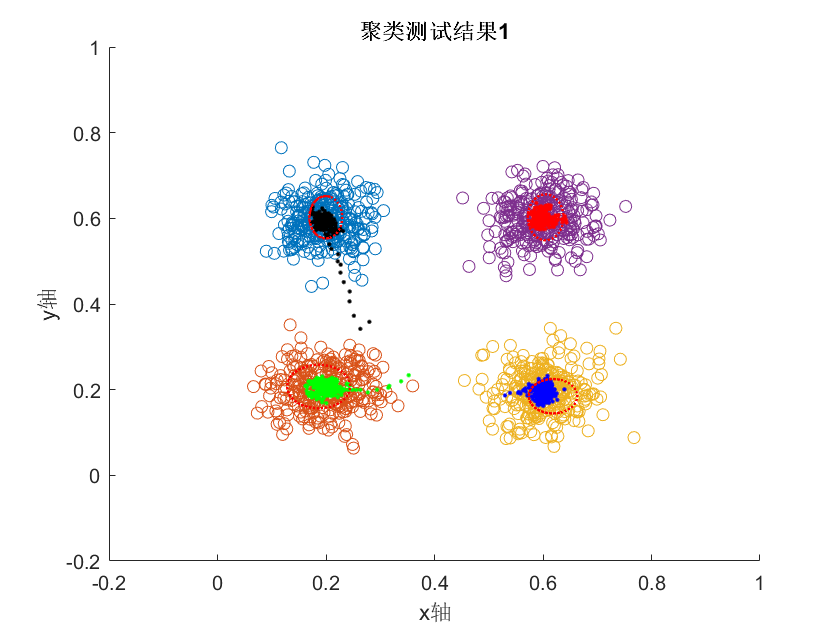
\includegraphics[width=0.7\textwidth]{ClusterTest1Result.png} % requires the graphicx package
   \caption{聚类测试1:理想状况,结果图}
   \label{fig:clustest1re}
\end{figure}

可见聚类效果比较理想。图\ref{fig:clustest1re}中红色椭圆展示了方差的情况,椭圆的圆心位置即为最终聚类的中心位置。而小圆点反映出每一个聚类随着样本逐一输入的的迁移情况。

我们对比最终聚类得到的参数结果和团簇真实值如下:
\begin{table}[htbp]
\centering
\begin{tabular}{c|c||c|c}
  \hline
  $\mu_{real}$   &  $\sigma_{real}$ &  $\mu$  &   $\sigma$\\
  \hline
  $(0.2,0.2)$    &  $(0.05,0.05)$   &  $(0.1864, 0.2073)$  & $(0.0580, 0.0508)$ \\
  $(0.2,0.6)$    &  $(0.05,0.05)$   &  $(0.1997, 0.6025)$  & $(0.0302, 0.0494)$ \\
  $(0.6,0.2)$    &  $(0.05,0.05)$   &  $(0.6185, 0.1847)$  & $(0.0446, 0.0401)$ \\
  $(0.6,0.6)$    &  $(0.05,0.05)$   &  $(0.6048, 0.6025)$  & $(0.0328, 0.0536)$ \\
  \hline
\end{tabular}
\caption{聚类测试1:聚类结果比较}
\label{tab:clustest1}
\end{table}

\subsubsection{常规测试}
接下来,我们采用默认参数进行训练;此时团簇之间存在交叠,并且方差不均一,在两个温度上不对称(见表\ref{tab:clusterpara})。之后的测试团簇的参数不再改变,我们将样本情况画出(符合之后所有的测试样本的情况)。

\begin{figure}[htbp]
   \centering
   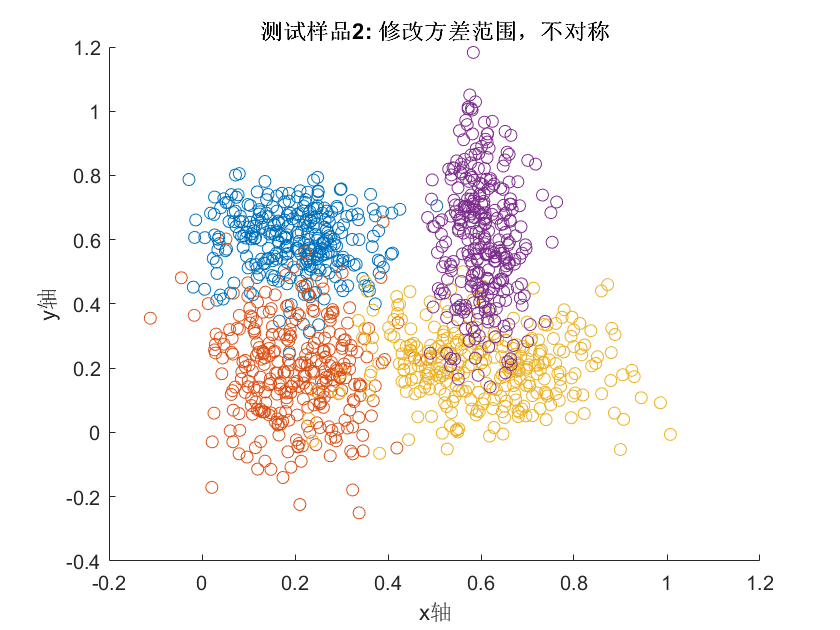
\includegraphics[width=0.7\textwidth]{ClusterTest2Sample.png} % requires the graphicx package
   \caption{聚类测试2:常规测试,样本图}
   \label{fig:clustest2sa}
\end{figure}

测试的结果如图\ref{fig:clustest2re}。

\begin{figure}[htbp]
   \centering
   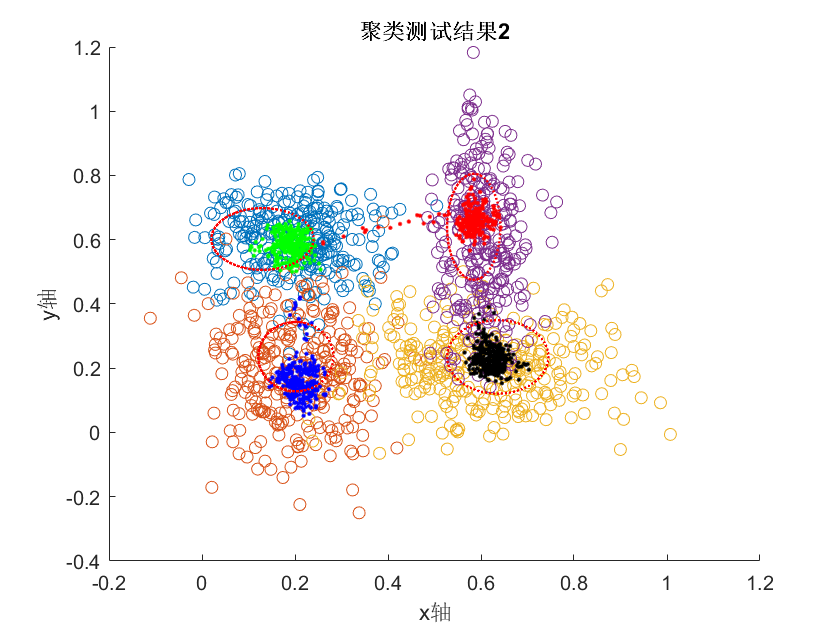
\includegraphics[width=0.7\textwidth]{ClusterTest2Result.png} % requires the graphicx package
   \caption{聚类测试2:常规测试,结果图}
   \label{fig:clustest2re}
\end{figure}

聚类效果仍然不错。方差的结果也比较符合数据的情况。
我们对比最终聚类得到的参数结果和团簇真实值如下:
\begin{table}[htbp]
\centering
\begin{tabular}{c|c||c|c}
  \hline
  $\mu_{real}$   &  $\sigma_{real}$ &  $\mu$  &   $\sigma$\\
  \hline
  $(0.2,0.2)$    &  $(0.1,0.15)$   &  $(0.2017, 0.2362)$  & $(0.0807, 0.1078)$ \\
  $(0.2,0.6)$    &  $(0.1,0.1)$   &  $(0.1301, 0.6024)$  & $(0.1097, 0.0961)$ \\
  $(0.6,0.2)$    &  $(0.15,0.1)$   &  $(0.6360, 0.2353)$  & $(0.1089, 0.1143)$ \\
  $(0.6,0.6)$    &  $(0.05,0.2)$   &  $(0.5844, 0.6403)$  & $(0.0573, 0.1648)$ \\
  \hline
\end{tabular}
\caption{聚类测试2:聚类结果比较}
\label{tab:clustest2}
\end{table}

\subsubsection{起始点位置变化的影响}
接下来,我们尝试改变起始点的位置,让起始点距离团簇较远,观察四个聚类中心是不是仍然能够捕捉到四个数据团簇的位置。

首先,我们将$\mu$初始化的范围移动到$(1,2)$,观测其聚类结果,如图\ref{fig:clustest3re}。

\begin{figure}[htbp]
   \centering
   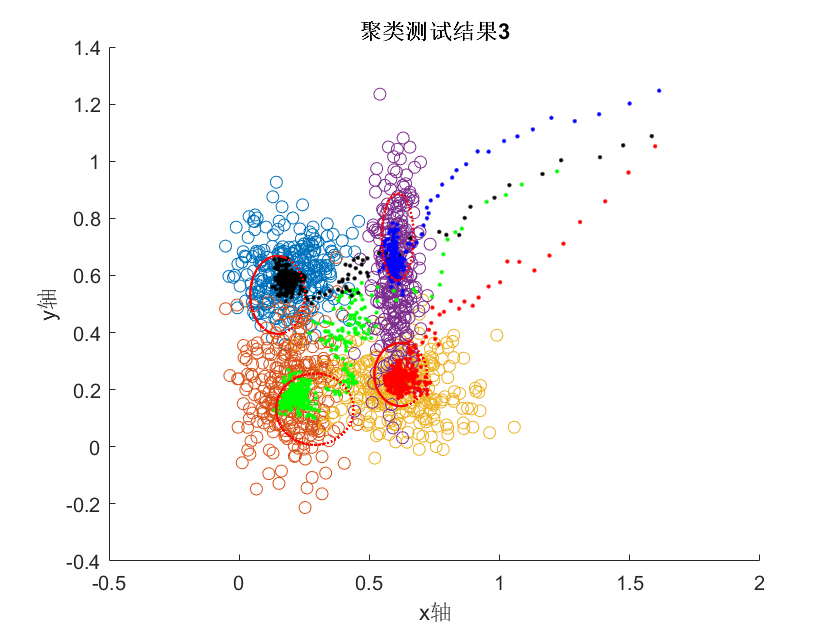
\includegraphics[width=0.7\textwidth]{ClusterTest3Result.png} % requires the graphicx package
   \caption{聚类测试3:起始点移动,结果图}
   \label{fig:clustest3re}
\end{figure}

可以发现其聚类效果仍然非常不错。聚类结果见表\ref{tab:clustest3},可见虽然中心存在一些偏差,但是已经准确地捕获到了聚类;如果输入更多数据将会改善其结果。数据方差值其实经历了一个先增大后减小的过程。
\begin{table}[htbp]
\centering
\begin{tabular}{c|c||c|c}
  \hline
  $\mu_{real}$   &  $\sigma_{real}$ &  $\mu$  &   $\sigma$\\
  \hline
  $(0.2,0.2)$    &  $(0.1,0.15)$   &  $(0.2905, 0.1316)$  & $(0.1482, 0.1250)$ \\
  $(0.2,0.6)$    &  $(0.1,0.1)$   &  $(0.1474, 0.5316)$  & $(0.1049, 0.1362)$ \\
  $(0.6,0.2)$    &  $(0.15,0.1)$   &  $(0.6200, 0.2530)$  & $(0.1011, 0.1103)$ \\
  $(0.6,0.6)$    &  $(0.05,0.2)$   &  $(0.6086, 0.7344)$  & $(0.0614, 0.1522)$ \\
  \hline
\end{tabular}
\caption{聚类测试3:聚类结果比较}
\label{tab:clustest3}
\end{table}

我们再将起始点范围更改为$(-5,0)$,其仍然可以很好的聚类,见图\ref{fig:clustest3-2re}。我们不再列出其参数结果。

\begin{figure}[htbp]
   \centering
   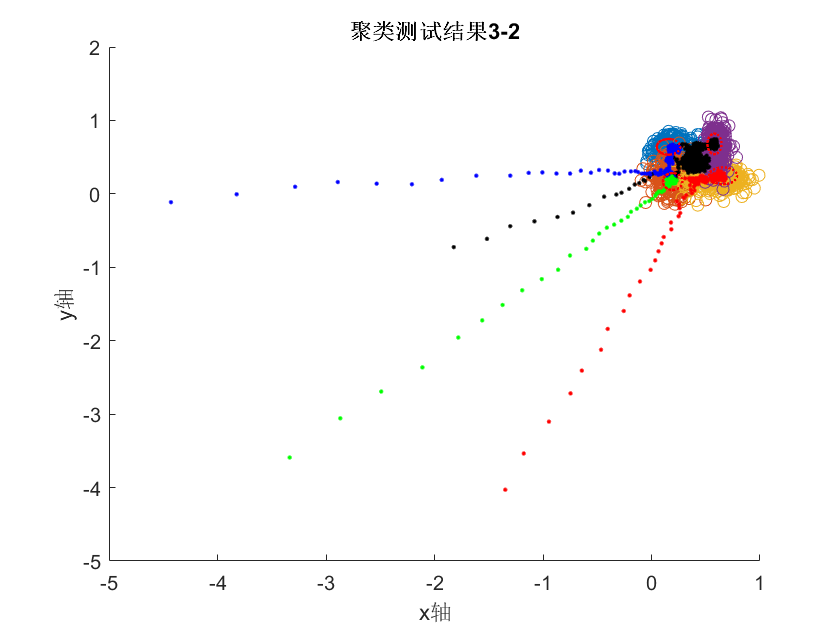
\includegraphics[width=0.7\textwidth]{ClusterTest32Result1.png} % requires the graphicx package
   \caption{聚类测试3-2:起始点大移动,结果图}
   \label{fig:clustest3-2re}
\end{figure}

\subsubsection{学习参数变化的影响}
学习参数$\alpha,\beta,\gamma$的选择是我们很关心的问题。学习参数在多大的范围内会对于聚类结果影响不敏感,这直接决定我们后期硬件设计是否要将其设置为变量的问题。

我们进行了多组$\alpha,\beta,\gamma$的测试,结果表明当$\alpha:0.05\sim 0.2,\;\beta:0.05\sim 0.2, \gamma: 0.95\sim 0.99$之间时,聚类效果较好,结果相对稳定。

图\ref{fig:clustest4re}展示$\alpha=0.2,\beta=0.2,\gamma=0.98$时的结果。

\begin{figure}[htbp]
   \centering
   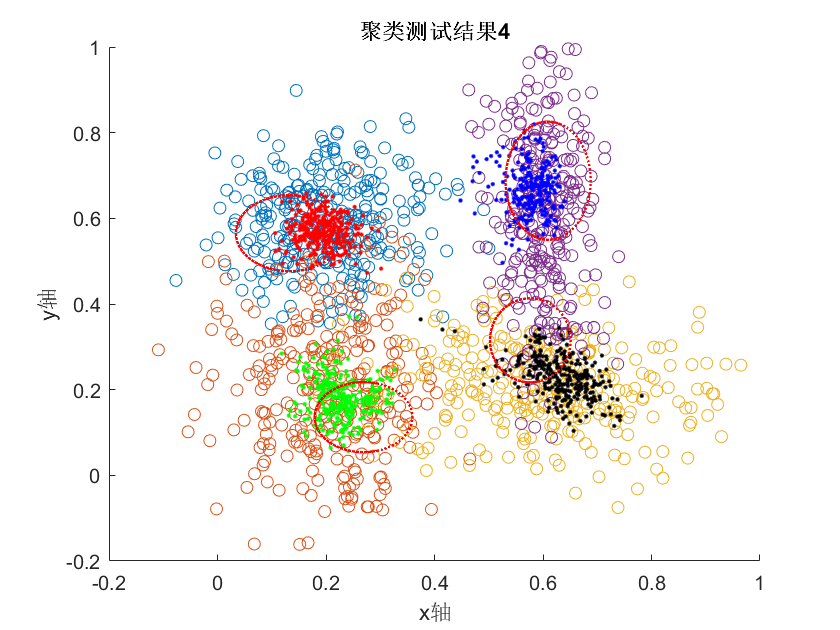
\includegraphics[width=0.7\textwidth]{ClusterTest4Result.png} % requires the graphicx package
   \caption{聚类测试4:学习参数调整,结果图}
   \label{fig:clustest4re}
\end{figure}

\begin{table}[htbp]
\centering
\begin{tabular}{c|c||c|c}
  \hline
  $\mu_{real}$   &  $\sigma_{real}$ &  $\mu$  &   $\sigma$\\
  \hline
  $(0.2,0.2)$    &  $(0.1,0.15)$   &  $(0.2692, 0.1358)$  & $(0.0901, 0.0818)$ \\
  $(0.2,0.6)$    &  $(0.1,0.1)$   &  $(0.1332, 0.5653)$  & $(0.0993, 0.0887)$ \\
  $(0.6,0.2)$    &  $(0.15,0.1)$   &  $(0.5766, 0.3151)$  & $(0.0743, 0.0981)$ \\
  $(0.6,0.6)$    &  $(0.05,0.2)$   &  $(0.6094, 0.6878)$  & $(0.0614, 0.1522)$ \\
  \hline
\end{tabular}
\caption{聚类测试4:聚类结果比较}
\label{tab:clustest4}
\end{table}

\subsubsection{聚类中心数目变化的影响}
聚类中心数目变化也是一个很重要的问题。 硬件设计时,很难考虑聚类数目随着数据灵活变化的问题;我们希望在聚类数目和真实的团簇数不一致的时候,聚类也能够有效地反映真实情况。

我们分别考虑聚类中心变多和变少两种情况。我们维持数据团簇数目$J_{real}=4$。

首先,我们令$J = 6$。聚类的结果如图\ref{fig:clustest5re}。

\begin{figure}[htbp]
   \centering
   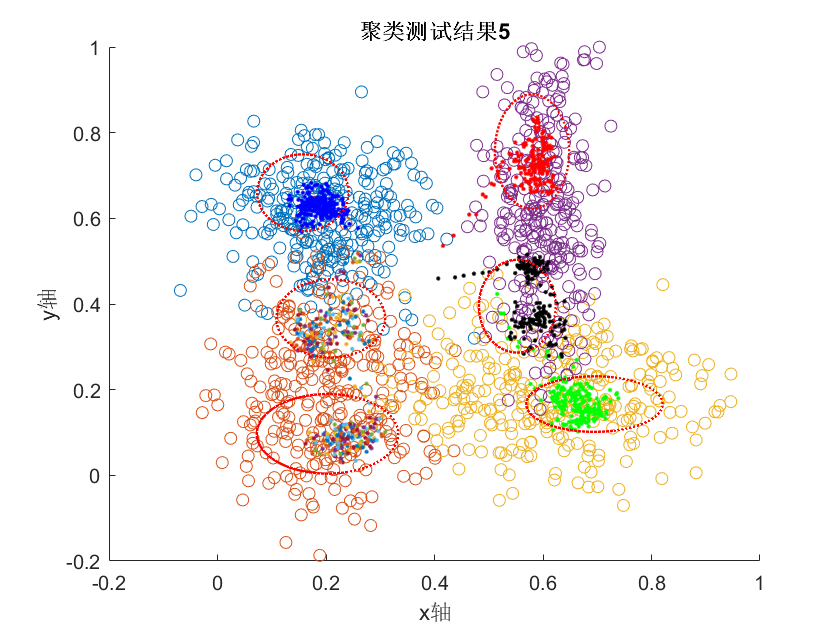
\includegraphics[width=0.7\textwidth]{ClusterTest5Result.png} % requires the graphicx package
   \caption{聚类测试5:聚类数目变多,结果图}
   \label{fig:clustest5re}
\end{figure}

可见聚类中心偏离了团簇的真实位置。然而,虽然聚类中心“过拟合”了团簇的真实情况,其对聚类的反映仍然基本正确。表列出了其聚类参数。

\begin{table}[htbp]
\centering
\begin{tabular}{c|c||c|c}
  \hline
  $\mu_{real}$   &  $\sigma_{real}$ &  $\mu$  &   $\sigma$\\
  \hline
  $(0.2,0.2)$    &  $(0.1,0.15)$   &  $(0.2088, 0.3663)$  & $(0.1002, 0.0913)$ \\
  $(0.2,0.6)$    &  $(0.1,0.1)$   &  $(0.1574, 0.6599)$  & $(0.0843, 0.0895)$ \\
  $(0.6,0.2)$    &  $(0.15,0.1)$   &  $(0.6849, 0.1664)$  & $(0.1256, 0.0649)$ \\
  $(0.6,0.6)$    &  $(0.05,0.2)$   &  $(0.5798, 0.7558)$  & $(0.0684, 0.1334)$ \\
  --    &  --   &  $(0.5527, 0.3949)$  & $(0.0708, 0.1083)$ \\
  --    &  --   &  $(0.2028, 0.0968)$  & $(0.1312, 0.0929)$ \\
  \hline
\end{tabular}
\caption{聚类测试5:聚类结果比较}
\label{tab:clustest5}
\end{table}

然后,我们减少聚类的个数,令$J = 2$。图\ref{fig:clustest5-2re}为两个聚类时的测试结果。可以看出聚类效果不是很理想,两个聚类中心不能找到任何一个特定的聚类中心,方差较大。
\begin{figure}[htbp]
   \centering
   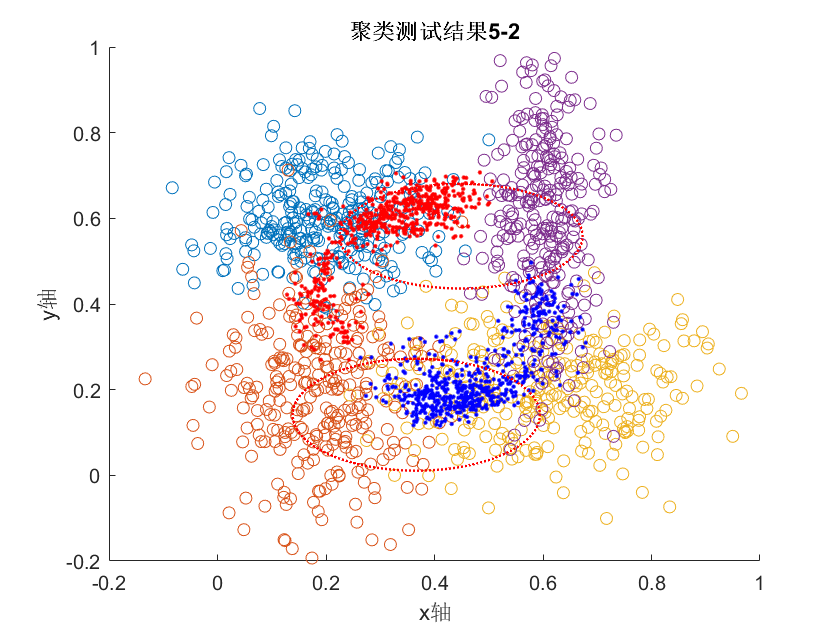
\includegraphics[width=0.7\textwidth]{ClusterTest52Result.png} % requires the graphicx package
   \caption{聚类测试5-2:聚类数目变少,结果图}
   \label{fig:clustest5-2re}
\end{figure}

聚类中心结果如表\ref{tab:clustest5-2}。

\begin{table}[htbp]
\centering
\begin{tabular}{c|c||c|c}
  \hline
  $\mu_{real}$   &  $\sigma_{real}$ &  $\mu$  &   $\sigma$\\
  \hline
  $(0.2,0.2)$    &  $(0.1,0.15)$   &  $(0.4491, 0.5583)$  & $(0.2239, 0.1222)$ \\
  $(0.2,0.6)$    &  $(0.1,0.1)$   &  $(0.3664, 0.1415)$  & $(0.2278, 0.1307)$ \\
  $(0.6,0.2)$    &  $(0.15,0.1)$   &  --  & -- \\
  $(0.6,0.6)$    &  $(0.05,0.2)$   &  --  & -- \\
  \hline
\end{tabular}
\caption{聚类测试5-2:聚类结果比较}
\label{tab:clustest5-2}
\end{table}

\subsubsection{聚类测试小结}
至此,我们总结出聚类的规律如下:
\begin{enumerate}
\item 起始位置对于聚类结果的影响很小;但是当数据点量较小时,将起始点初始化在数据范围内会使得其对聚类的捕捉更为迅速;
\item 在一定范围内(本实验为$\alpha:0.05\sim 0.2,\;\beta:0.05\sim 0.2, \gamma: 0.95\sim 0.99$),学习速率对聚类最终的结果影响不大,结果较为稳定;
\item 聚类数目比实际聚类数要多时,聚类的方差较小,对真实聚类情况能够有所反映;而聚类数目偏少时,不太能够有效地反映聚类的情况。后续测试应该将聚类数尽量设得多一些。
\end{enumerate}


\subsection{MNIST手写数字识别测试}
接下来我们进行了静态图像的识别测试。MNIST是一个常用的检测学习算法效果的手写数字集库。

在以下测试中,我们使用的DeSTIN结构为:
\begin{enumerate}
\item 底层输入层包含4*4个神经元,每个底层神经元接收底层图像4*4小单元的输入以及自身信度状态的反馈;底层神经元具有25个聚类;那么其输入维度为41维,输出维度为25维;底层的“视觉窗口”为16*16维;
\item 非底层神经元接收下属四个底层神经元的输入以及自身信度状态的反馈;同样地,其具有25个聚类;那么其输入维度为125维,输出维度为25维;
\item 整个DeSTIN结构分为3层:底层4*4,中间层2*2和顶层1*1,共21个神经元;
\item 在非底层神经元接收底层神经元信度状态输入的时候,底层神经元可以接收新图片的输入,构成流水线结构,如图\ref{fig:pipeline}。
\end{enumerate}

\begin{figure}[htbp]
   \centering
   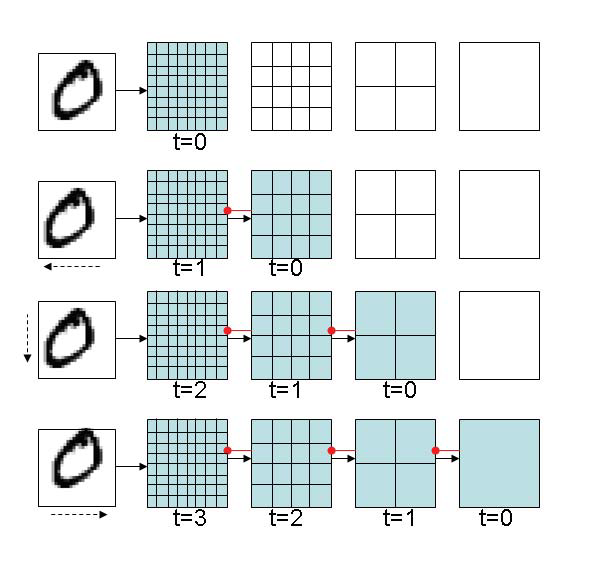
\includegraphics[width=0.7\textwidth]{ScanningPipeline.png} % requires the graphicx package
   \caption{DeSTIN结构与流水线}
   \label{fig:pipeline}
\end{figure}


\subsubsection{深度学习网络基本测试流程}
我们首先来介绍一下在使用DeSTIN(或者其他深度学习特征提取网络)进行数据测试的基本过程。首先,我们需要具有大量的无标签的数据,以及少量有标签的数据。我们将数据分为\uline{无标签训练集,有标签训练集,有标签测试集}三个部分。

那么,整个训练将分为三个步骤:
\begin{enumerate}
\item 通过大量无标签数据,训练DeSTIN网络,让其产生较好的聚类结果,如图\ref{fig:step1};
\item 关闭DeSTIN网络的训练,输入有标签的训练数据,训练后面的监督学习网络(本文中我们采用二层普通神经网络),如图\ref{fig:step2};
\item 关闭监督学习网络的训练,输入测试数据,测试其预测的结果,如图\ref{fig:step3};
\end{enumerate}

\begin{figure}[htbp]
   \centering
   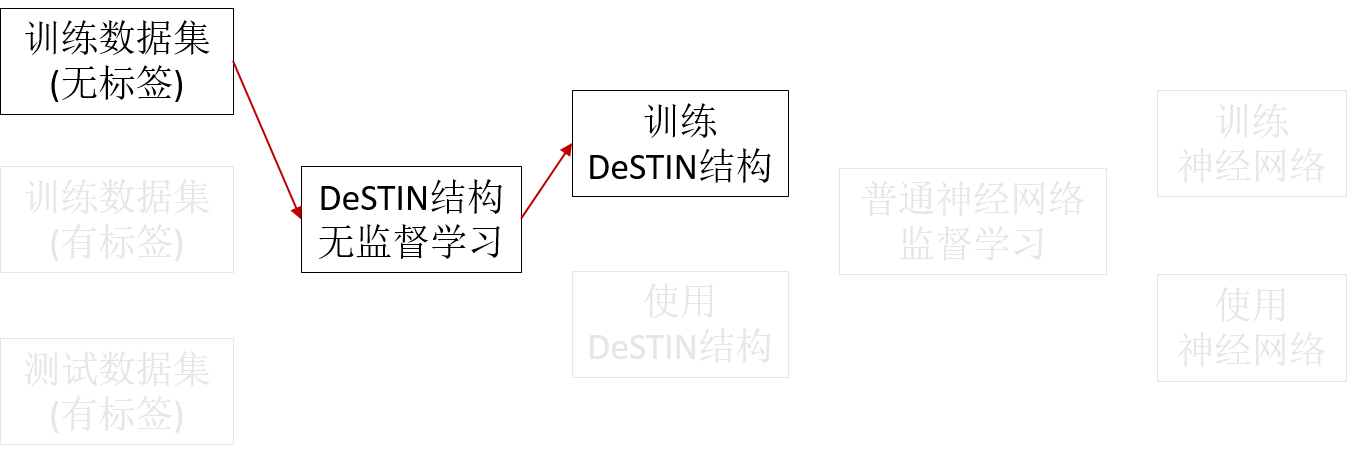
\includegraphics[width=0.7\textwidth]{DeSTINStep1.png} % requires the graphicx package
   \caption{测试过程1:无监督网训练}
   \label{fig:step1}
\end{figure}

\begin{figure}[htbp]
   \centering
   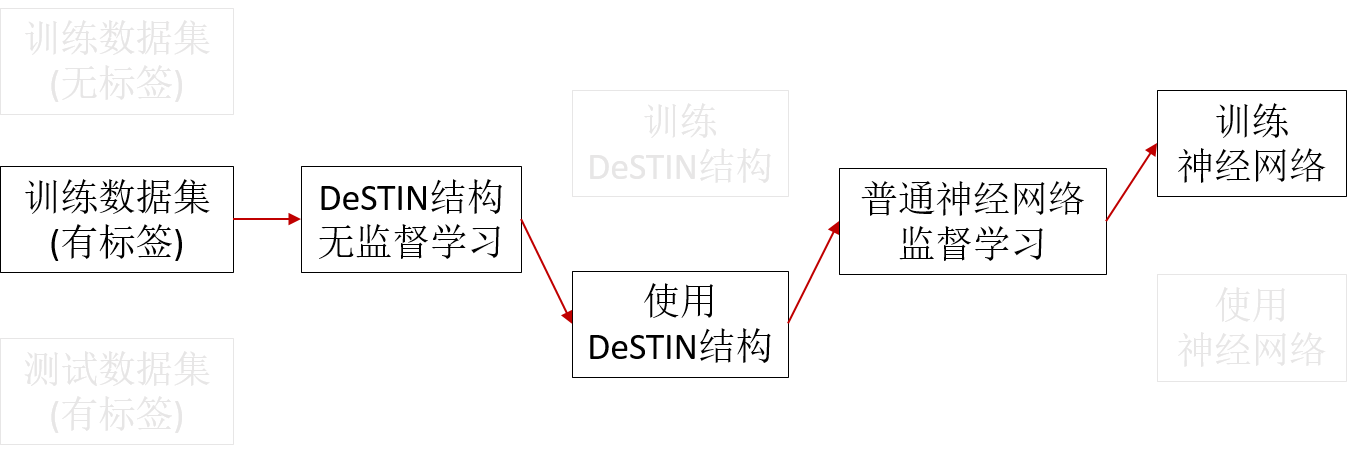
\includegraphics[width=0.7\textwidth]{DeSTINStep2.png} % requires the graphicx package
   \caption{测试过程2:有监督网训练}
   \label{fig:step2}
\end{figure}

\begin{figure}[htbp]
   \centering
   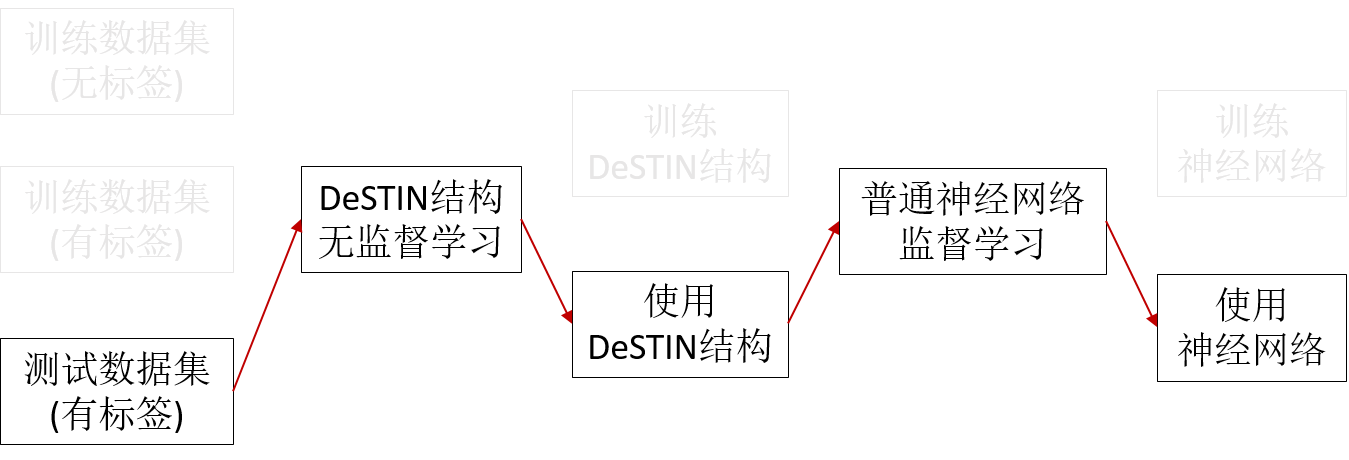
\includegraphics[width=0.7\textwidth]{DeSTINStep3.png} % requires the graphicx package
   \caption{测试过程3:预测过程}
   \label{fig:step3}
\end{figure}

\subsubsection{扫描方法的采用}
根据之前的分析,我们采用的DeSTIN算法在用来进行时间序列问题处理时比较合理,那么如何将其应用到静态图像识别上去呢?

在此我们借鉴了一个“视觉扫描”的理论:当人眼在看一件物品时,其注意中心是在进行不断的快速扫描的,这样可以防“视网膜”抖动,保持较高的分辨能力\cite{Deubel1996Postsaccadic}。

在这里我们模仿人眼的处理过程,让DeSTIN底层的“数据接收窗口”按照一个固定的顺序读取图像的每一个部分,这样就可以将静态的图像转换为动态的序列\cite{Karnowski2012Deep}。

此处我们首先采用简化的MNIST数据集,每一张手写数字图像为$20\times 20$像素点,我们架构的DeSTIN网络的“视觉窗口”为$16\times 16$那么我们采取图\ref{fig:scanning}的扫描方法,即让视觉窗口按照图示顺序平移,在进行到画圈处的时候,输出相应的信度状态。

\begin{figure}[htbp]
   \centering
   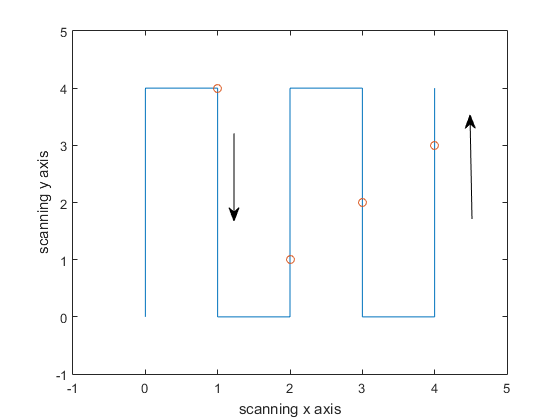
\includegraphics[width=0.7\textwidth]{ScanningImage.png} % requires the graphicx package
   \caption{“视觉扫描”识别的扫描顺序}
   \label{fig:scanning}
\end{figure}

我们将学习参数设置为$\alpha = 0.125, \beta = 0.125, \gamma = 0.9984$(第四章详细讲这样设置的原因)。测试集中,读入图片的前100张和相应的信度状态(前100维)的图像分别如\ref{fig:scanning}和图\ref{fig:belief}。

\begin{figure}[htbp]
   \centering
   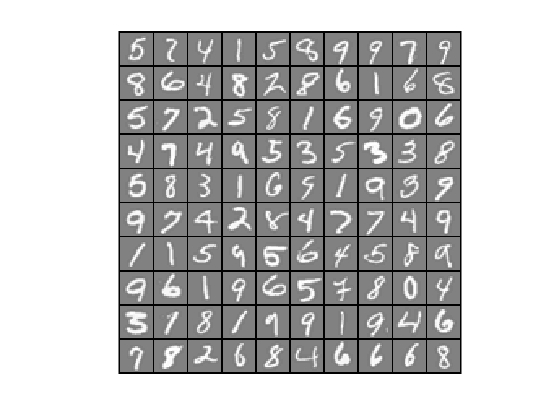
\includegraphics[width=0.7\textwidth]{MNISTSample.png} % requires the graphicx package
   \caption{MNIST测试的数字样本}
   \label{fig:scanning}
\end{figure}


\begin{figure}[htbp]
   \centering
   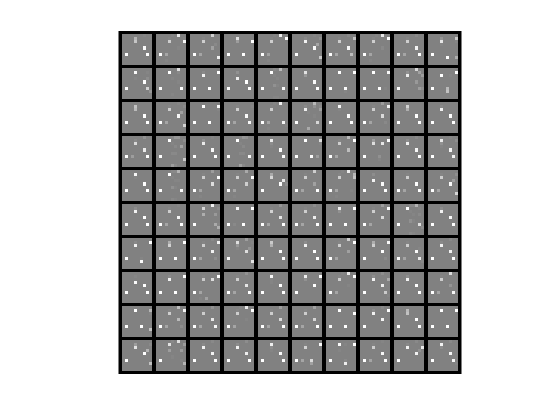
\includegraphics[width=0.7\textwidth]{MNISTResult.png} % requires the graphicx package
   \caption{MNIST测试DeSTIN网络输出的信度状态}
   \label{fig:belief}
\end{figure}

对于监督学习过程,我们采用普通的二层神经网络。 DeSTIN网络进行MNIST数据集测试训练的MATLAB代码将附在附录里面。我们得到了97.3\%的准确率。这说明我们的DeSTIN网络效果比较理想。

\subsubsection{学习参数变化测试}
我们再次在MNIST测试中测试结果对于学习参数的敏感情况。

首先,我们固定$\alpha = 0.125, \beta = 0.125$,改变$\gamma$,测试其准确率的变化如图\ref{fig:starverate}。可见当$\gamma:0.97\sim 0.99$时其准确度较高。

\begin{figure}[htbp]
   \centering
   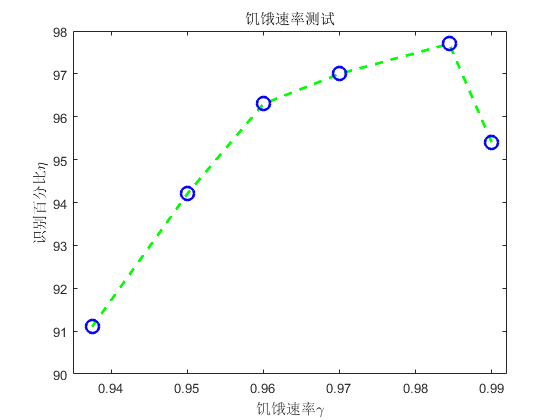
\includegraphics[width=0.7\textwidth]{StarveRate.png} % requires the graphicx package
   \caption{饥饿速率对准确度的影响}
   \label{fig:starverate}
\end{figure}

然后,我们固定$\gamma=0.9844$,在$0.05\sim 0.225$范围内,以$0.025$为步长遍历整个$\alpha,\beta$参数空间,最终获得的参数测试结果如图\ref{fig:learningrate}。

\begin{figure}[htbp]
   \centering
   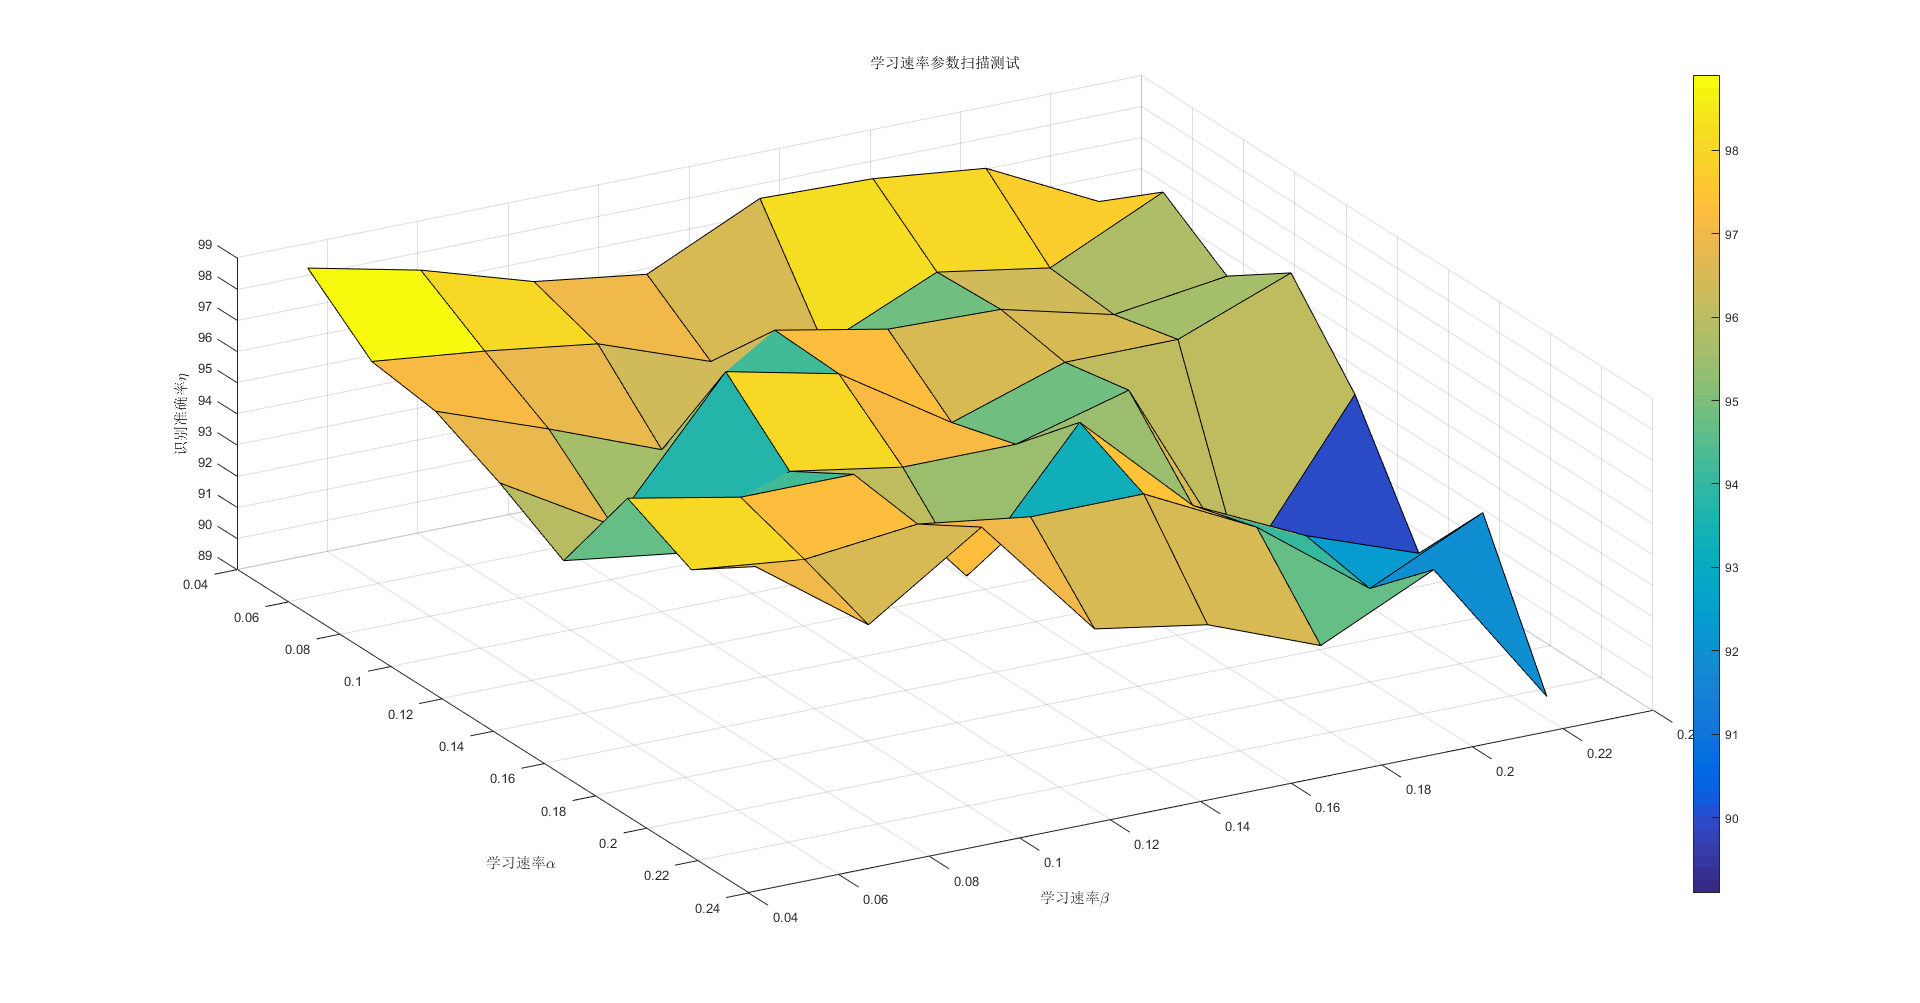
\includegraphics[width=\textwidth]{LearningRate.png} % requires the graphicx package
   \caption{学习速率对准确度的影响}
   \label{fig:learningrate}
\end{figure}

可见在$0.05\sim 0.2$的范围以内,学习速率对准确度影响很有限。考虑进方差的因素后,我们可以认为,准确度在此范围内对于学习速率不敏感。 这和前面聚类测试结果相吻合。

%\subsection{PEMS-SF数据集动态识别测试}
%动态识别仍在进行中,估计二稿整理出来

我们同样进行了标准的$28\times 28$大图像MNIST的测试,结果可以保持在$96\%$左右,同样相当理想。

\subsection{CIFAR物体识别测试与改进}
接下来我们想进行更加困难的测试:彩色物体识别。CIFAR是一个大型的彩色自然图像数据库\cite{CIFAR-10},其物体涵盖了大种类20种;小种类接近100种。其图像尺寸为$32\times 32\times 3$。图\ref{fig:cifar}展示了数据训练集的前100张图片。

\begin{figure}[htbp]
   \centering
   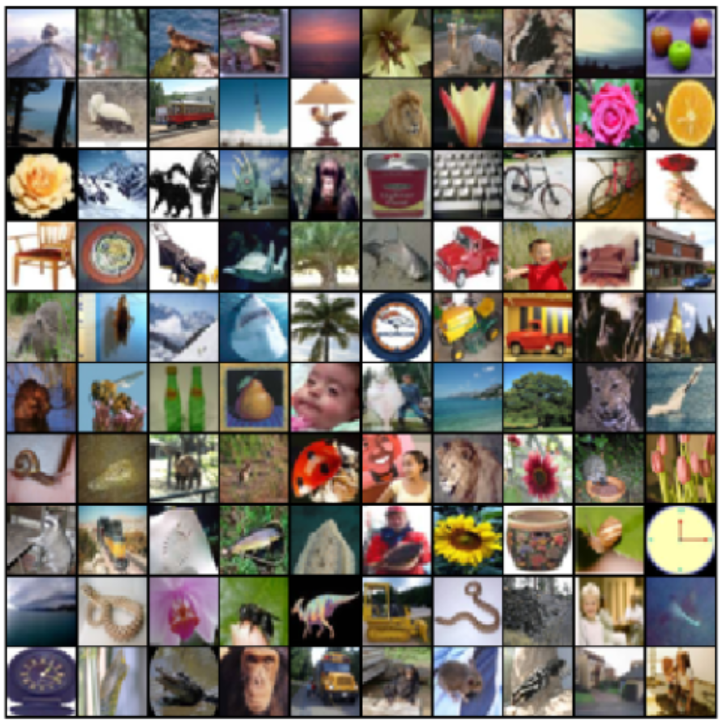
\includegraphics[width=0.7\textwidth]{cifar.png} % requires the graphicx package
   \caption{CIFAR数据集图例}
   \label{fig:cifar}
\end{figure}

我们按照MNIST的类似思路进行了CIFAR图像的训练(参考了Github上有关的Python代码\cite{pythonDeSTIN}),监督学习仍然使用了二层神经网络。

然而,我们最终只做出了最高$20.1\%$的准确度。

通过分析CIFAR测试失败的原因,我们发现的DeSTIN算法的固有缺陷:\textbf{对于位置的依赖关系严重}。当我们进行静态“扫描”识别的时候,很容易想象到,如果一个特征的位置发生了很大的变动:或者说,翻转、扭曲,这时候原来系统提取到的特征便不再吻合变化之后的物体。然而CIFAR数据集物体的位置特征比较混乱,这就导致识别的准确度大大降低。

我们在第二章讨论过有关\uline{卷积神经网络}的基本概念;卷积神经网络最早提出时,正是考虑到了我们刚刚讨论到的问题,认为\uline{一个图像内部的特征不会因为其线性变换而发生改变},因而提出了\uline{通过卷积核反映特征,卷积核对整个图像做卷积提取特征}的想法。

下一步我们对于DeSTIN算法将进行改进,在DeSTIN算法前面加上一层卷积、池化层,这样算法测试的结果应当能够得到较大改善。

%\bibliography{reference}
\chapter{专用电路设计与仿真}\label{chapter_design}
\graphicspath{{chapter4/figure/}}

通过一系列的算法测试,我们可以确认常规的DeSTIN算法在\uline{图像特征位置变化不明显}时进行静态、动态识别的准确度较高。 本章我们介绍基于DeSTIN算法,我们进行的\uline{单个神经元结构}的硬件设计工作:包括数据的量化测试、数字电路框架的设计以及数字电路的聚类测试仿真结果。

我们目前的硬件设计主要基于一个\uline{二维数据输入,内部四个聚类的单个神经元}。 

\section{定点数聚类测试}
采用定点数框架是因为其更容易在小型电路上实现,运算单元相对简单。大多数专用电路设计均采用定点数框架。

定点数测试是硬件设计的第一步。此时我们要将抽象的数转变为电路中的一组高低电平信号来考虑,将每一步算数运算考虑成电路中的一个逻辑运算单元。 尤其是对于乘法、除法,我们要考虑到牺牲精度后带来的影响以及溢出后是否较为严重地影响结果。

\subsection{定点数测试中注意的修改}
\subsubsection{数据的量化} 
在进行软件层次上的算法测试时,我们计算的对象都是$double$型双精度的浮点数;虽然浮点数运算过程复杂、耗费计算量,其运算范围广泛并且能够很好地保证精度,因而我们不用过于考虑算法具体实现上的“噪音”问题。

在我们今后的考虑中,不再有“数”这个抽象的概念。我们考虑的都是一组记录高电平、低电平的电线或者寄存器。我们进行每一步运算时,都要将其对应到底层高低电平的相互转换。

通过平衡计算资源与表示精度的需求,我们将数据的\textbf{二进制长度限制在16bit},也就是说,每一个数用16个高低电平来表示。 我们\textbf{小数位数控制为14位},并采用补码的编码方法,这样我们可以表示的数的范围便是:$-2\sim 1.999$,能够表示的最小精度是$6.1035*10^{-5}$。

采取补码进行运算时有很多"Trick",包括乘法、加法溢出的处理,正负数之间进行每一种运算的结果是否正确,在此不便赘述。

\subsubsection{运算合并与整理}
对于所有运算来说,最消耗计算资源、也是最消耗计算时间的计算之一便是除法。Fourier变换之所以能够产生快速算法,是因为其只涉及加法、乘法。我们希望在硬件设计之前,重新检查我们的算数运算内容,进行相应的整理、归并,减少运算次数,尤其是除法的运算次数。

首先,我们想到的是\uline{特定学习速率、饥饿速率的选择}的问题。当我们选择$\alpha = 0.125\;(=\dfrac{1}{8}),\beta = 0.125\;(=\dfrac{1}{8}), \gamma = 0.9844 \;(= 1- \dfrac{1}{64})$时,出现了大量的\uline{2的幂次},那么我们可以把所有的乘除法转化为左右移位的计算,省去了大量的计算复杂度。结合前面算法测试的经验,学习速率在这个范围以内对准确度不造成很大影响,也说明了这样处理的合理性。

其次,我们要检查残存除法的位置。 通过分析Online k-means聚类方法,我们发现其仍然有两部分存在除法:计算归一化距离$n$时每一个聚类存在一步除法(不可避免);最后计算Belief State时涉及大量除法。

当聚类数为4的时候,我们将计算Belief State的公式进行简化,有:

$$p_1 = \dfrac{\dfrac{1}{n_1}}{\dfrac{1}{n_1}+\dfrac{1}{n_2}+\dfrac{1}{n_3}+\dfrac{1}{n_4}} = \dfrac{n_2 n_3 n_4}{n_2 n_3 n_4 + n_1 n_3 n_4 + n_1 n_2 n_4 + n_1 n_2 n_3}$$

那么有:(我们用$a,b,c,d$作为下标)
\begin{equation}
p_a = \dfrac{n_b n_c n_d}{n_b n_c n_d + n_a n_c n_d + n_a n_b n_d + n_a n_b n_c}
\end{equation}

以上$a,b,c,d$可以轮换。我们只需先计算所有的三项乘积,计算其加和,再对每一个输出计算一次除法,除法的次数由2*J次缩减为J次。

\subsubsection{除法的实现: Cordic算法}

对于不可规避的除法,我们采用了一种Cordic(COordinate Rotation DIgital Computer)算法,这是一种空间资源消耗少的,简单易行的算法。 其基本原理基于一个三角函数公式:
\begin{equation}
\begin{aligned}
K_n R sin(\theta \pm \phi) & = & R sin(\theta) \pm 2^{-n} R cos(\theta) \\
K_n R cos(\theta \pm \phi) & = & R cos(\theta) \mp 2^{-n} R sin(\theta) \\
with K_n = \sqrt{1+2^{-2n}} & , & tan(\phi) = 2^{-n} 
\end{aligned}
\end{equation}

我们主要采用其在除法运算上的变体--属于"移位加"算法类的一种。主要思想是“多退少补”,不断将被除数右移,计算商更精确的位数。

我们将Cordic除法的MATLAB代码展示出来。
\begin{spacing}{1}
\begin{lstlisting}[language=Matlab][deletekeywords={input, beta, gamma}]
function zin = cordic_div(yin, xin)
%% Cordic Division Fixed Point Version
% By Pei Zeng, PHY, NJU, 05/12/2016
% numerictype: Ty = numerictype('WordLength',16,'FractionLength',14)
% NOTICE: the input divident yin should be SMALLER than the input division
% xin!!!

%% Testbench Setting
Ty = numerictype('WordLength',16,'FractionLength',14);  % for fixed point type
F = globalfimath('CastBeforeSum',0,'OverflowAction','Saturate',...
    'RoundingMethod','Floor', 'ProductMode','SpecifyPrecision'...    
    ,'ProductWordLength',16,'ProductFractionLength',14,... 
    'SumMode','SpecifyPrecision'...    
    ,'SumWordLength',16,'SumFractionLength',14);  % for global fixed math operation setting
P = fipref('NumberDisPlay','RealWorldValue','NumericTypeDisplay','full');  % for afterwards realworld number display

%% Cordic
iter = Ty.WordLength - 1;
% convert to fixed point if not
xin = fi(xin, Ty);
yin = fi(yin, Ty);
zin = fi(0, Ty);

for j=0:iter
        if(yin < 0)
                alpha = fi(1,Ty);
        else
                alpha = fi(-1,Ty);
        end
         
        y = yin + alpha * 2^(-j) * xin;
        z = zin - alpha * 2^(-j);
         
        %matrix(j+1,:) = [j yin alpha xin zin];
        
        yin = y;
        zin = z;
end
\end{lstlisting}
\end{spacing}


\subsection{定点数测试结果}
在做完以上修改后,我们重新在MATLAB平台上进行聚类测试。此处我们用到了MATLAB的定点仿真工具箱Fixed Point Toolbox,其用于模拟定点数的运算情况。我们将乘法溢出设置为"饱和",这样如果定点数相乘超过2,结果会停留在1.999的最大值上。这符合我们后面硬件计算的乘法设定。

进行定点数测试的代码如下:

\begin{spacing}{1}
\begin{lstlisting}[language=Matlab][deletekeywords={input, beta, gamma}]
%% MATLAB fixed point test -- Online Clustering
% Pei Zeng, PHY, NJU, 05/12/2016
% Testbench Setting
Ty = numerictype('WordLength',16,'FractionLength',14);  % for fixed point type
F = globalfimath('CastBeforeSum',0,'OverflowAction','Saturate',...
    'RoundingMethod','Floor', 'ProductMode','SpecifyPrecision'...    
    ,'ProductWordLength',16,'ProductFractionLength',14,... 
    'SumMode','SpecifyPrecision'...    
    ,'SumWordLength',16,'SumFractionLength',14);  % for global fixed math operation setting
P = fipref('NumberDisPlay','RealWorldValue','NumericTypeDisplay','full');  % for afterwards realworld number display


% Sample Generation
n=300;
x1 = 0.2; y1 = 0.6; sigma1x = 0.1; sigma1y = 0.1;
x2 = 0.2; y2 = 0.2; sigma2x = 0.1; sigma2y = 0.15;
x3 = 0.6; y3 = 0.2; sigma3x = 0.15; sigma3y = 0.1;
x4 = 0.6; y4 = 0.6; sigma4x = 0.05; sigma4y = 0.2;

samp1 = fi([x1 + sigma1x * randn(n,1),y1 + sigma1y * randn(n,1)],Ty);
samp2 = fi([x2 + sigma2x * randn(n,1),y2 + sigma2y * randn(n,1)],Ty);
samp3 = fi([x3 + sigma3x * randn(n,1),y3 + sigma3y * randn(n,1)],Ty);
samp4 = fi([x4 + sigma4x * randn(n,1),y4 + sigma4y * randn(n,1)],Ty);

sample = [samp1;samp2;samp3;samp4];

scatter(samp1(:,1),samp1(:,2));
hold on;
scatter(samp2(:,1),samp2(:,2));
hold on;
scatter(samp3(:,1),samp3(:,2));
hold on;
scatter(samp4(:,1),samp4(:,2));
hold on;

title('Fixed Point Test');
xlabel('xlabel');
ylabel('ylabel');
axis([-0.2,1,-0.2,1])

% parameter initialization
training = 1;   %Turn on the training switch
%alpha = 0.125; beta = 0.125; gamma = 0.9844;    %Learning Parameter
alpha = fi(0.125,Ty); beta = fi(0.125,Ty); gamma = fi(0.9844,Ty);    %Learning Parameter

% neuron Initialization
mu = fi(0.15 + 0.5 * rand(2,4),Ty);
sigma2 = fi(ones(2,4),Ty);
starve = fi(ones(4,1),Ty);

%Neuron Parameter Record
Mu1 = fi(zeros(4*n, 2),Ty); Sigma1 = fi(zeros(4*n, 2),Ty);
Mu2 = fi(zeros(4*n, 2),Ty); Sigma2 = fi(zeros(4*n, 2),Ty);
Mu3 = fi(zeros(4*n, 2),Ty); Sigma3 = fi(zeros(4*n, 2),Ty);
Mu4 = fi(zeros(4*n, 2),Ty); Sigma4 = fi(zeros(4*n, 2),Ty);
Starve = fi(zeros(4*n, 4),Ty);

sample = sample(randperm(4*n),:);

%Training Process
for t = 1:(4*n)
    input = sample(t,:)';
    [belief, mu, sigma2, starve] = OnlineClustering(input, mu, sigma2, starve, alpha, beta, gamma, training);
    Mu1(t,:) = mu(:,1)';
    Mu2(t,:) = mu(:,2)';
    Mu3(t,:) = mu(:,3)';
    Mu4(t,:) = mu(:,4)';
    Starve(t,:) = starve';
end

%Plot
for t = 1:(4*n)
    plot(Mu1(t,1),Mu1(t,2),'r.',Mu2(t,1),Mu2(t,2),'b.',Mu3(t,1),Mu3(t,2),'g.',Mu4(t,1),Mu4(t,2),'k.');
    hold on;
end

% Plot Ellipse
DrawEllipse(mu(:,1),sigma2(:,1));
DrawEllipse(mu(:,2),sigma2(:,2));
DrawEllipse(mu(:,3),sigma2(:,3));
DrawEllipse(mu(:,4),sigma2(:,4));

\end{lstlisting}
\end{spacing}

其中online聚类算法代码如下:
\begin{spacing}{1}
\begin{lstlisting}[language=Matlab][deletekeywords={input, beta, gamma}]
function [belief, mu, sigma2, starve] = OnlineClustering(input, mu, sigma2,starve, alpha, beta, gamma, training)
%% Use Online k-means Clustering method to calculate the belief
%% Fixed Point Version
% Written by Pei Zeng, PHY, NJU
% Date 2016/05/12

% Data input to this function: 
% input: input data to the neuron. I-by-1 vector 
% (I is the input dimension,which is defined in DeSTIN.m)
% mu: centroid attribute for the coordinate of center. I-by-J vector
% (J is the belief dimension, which is defined in DeSTIN.m)
% sigma2: centroid attribute for the radius square. I-by-J vector

% New data output from this function:
% belief: new belief state of the neuron: J-by-1 vector

% initialization
I = size(input,1);
J = size(mu, 2);

%% Testbench Setting
Ty = numerictype('WordLength',16,'FractionLength',14);  % for fixed point type
F = globalfimath('CastBeforeSum',0,'OverflowAction','Saturate',...
    'RoundingMethod','Floor', 'ProductMode','SpecifyPrecision'...    
    ,'ProductWordLength',16,'ProductFractionLength',14,... 
    'SumMode','SpecifyPrecision'...    
    ,'SumWordLength',16,'SumFractionLength',14);  % for global fixed math operation setting
P = fipref('NumberDisPlay','RealWorldValue','NumericTypeDisplay','full');  % for afterwards realworld number display

%% Data Processing
% 1. Calculating the Euclidean distance from the input to each centroid
D_Euc = fi(zeros(J, 1),Ty);
for j = 1 : J
    D_Euc(j) = (input - mu(:,j))' * (input - mu(:,j));
end

% 2. Judge which cluster the input belongs to: Winner-take-all method
[~, j0] = min(starve .* D_Euc);

if (training == 1) % do the renewing only in the training process
% 3. Renew the starvation trace of each centroid
starve = starve * gamma;
starve(j0) = starve(j0) + (fi(1,Ty) - gamma);

% 4. Calculate the error for the centroid j0 and the input signal
Er_mu = input - mu(:,j0);
Er_sigma2 = (input - mu(:,j0)).* (input - mu(:,j0)) - sigma2(:,j0);

% 5. Learning Process: learning rate : alpha, beta
mu(:,j0) = mu(:,j0) + alpha * Er_mu;
sigma2(:,j0) = sigma2(:,j0) + beta * Er_sigma2;
end

% 6. Calculate the Mahanalobis distance: IMPORTANT
D_Mah = fi(zeros(J, 1),Ty);
% cordic_div version
for j = 1 : J
    for i = 1 : I
        D_Mah(j) = D_Mah(j) + cordic_div( (input(i) - mu(i,j))*(input(i) - mu(i,j)), sigma2(i,j) );
    end
end

% 7. "Inverse-normalize" the D_Mah values, and attain the new belief state
Multi = fi(ones(J, 1), Ty);
for j = 1 : J
    for k = 1: J
        if (k~=j)
            Multi(j) = Multi(j) * D_Mah(k);
        end
    end
end

Sum = sum(Multi);

% Cordic_div version belief calculation
belief = fi(zeros(J, 1), Ty); 
for j = 1 : J
    belief(j) = cordic_div(Multi(j), Sum);
end

\end{lstlisting}
\end{spacing}

最终的聚类测试结果仍然较为理想。我们附上同第三章常规测试的结果如图\ref{fig:fixedre}和表\ref{tab:clustestfix}。

\begin{figure}[htbp]
   \centering
   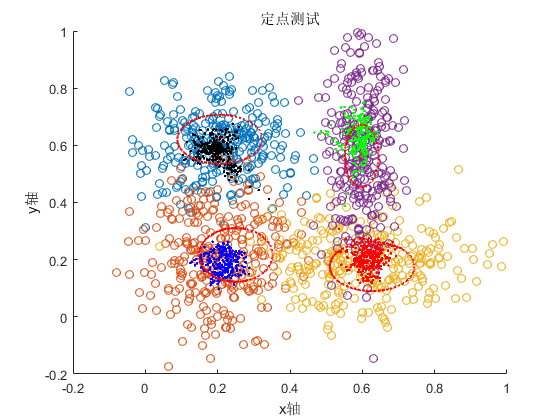
\includegraphics[width=0.7\textwidth]{FixedPointClustering.png} % requires the graphicx package
   \caption{定点测试:常规测试,结果图}
   \label{fig:fixedre}
\end{figure}

\begin{table}[htbp]
\centering
\begin{tabular}{c|c||c|c}
  \hline
  $\mu_{real}$   &  $\sigma_{real}$ &  $\mu$  &   $\sigma$\\
  \hline
  $(0.2,0.2)$    &  $(0.1,0.15)$   &  $(0.2501, 0.2169)$  & $(0.1172, 0.0859)$ \\
  $(0.2,0.6)$    &  $(0.1,0.1)$   &  $(0.2058, 0.6210)$  & $(0.1097, 0.0961)$ \\
  $(0.6,0.2)$    &  $(0.15,0.1)$   &  $(0.6271,0.1763)$  & $(0.0469, 0.1094)$ \\
  $(0.6,0.6)$    &  $(0.05,0.2)$   &  $(0.5983, 0.5628)$  & $(0.0573, 0.1648)$ \\
  \hline
\end{tabular}
\caption{定点聚类测试:聚类结果比较}
\label{tab:clustestfix}
\end{table}

对于$\sigma$误差过大,部分原因是我们运算中采用的是$\sigma^2$,因而上表得到的数据经过了一次定点数下的开方,而开放运算相当不准确。

在此有必要进行补充说明的是,我们是经历过多次数据量化方法的选择才最终确定“16位长度,14位小数”的结果的,所以说真实的调试过程是\uline{在"x位长度,y位小数"下进行MATLAB定点测试,最终因为较低精度,较少小数位导致结果不收敛或者报错;在尽可能少的位数要求下优化出了这个结果}。


\section{硬件结构设计}

我们通过定点测试得到了数据量化的基本要求以及除法的解决方案。接下来,我们进行了硬件的设计。

笔者将简要介绍自己设计的硬件结构的框架,然后介绍重要细节部分的实现方法;最终介绍细节部分的仿真结果。

\subsection{总体结构设计示意图}

如图\ref{fig:clusterframe},笔者采用Microsoft Visio进行制图。 整个硬件分为\textbf{神经单元,饥饿单元,比较器单元和信度计算单元}四个部分。

图\ref{fig:clusterframe}中每一列代表一个聚类,每一行代表一个输入数据维度;那么每一个聚类有I个神经单元和1个饥饿单元;总共J个聚类。每一个神经单元负责处理一个聚类某一维度的数据。

数据首先通过\uline{Input Bus}进入到每个神经单元,神经单元计算出其与data之间的Euclid距离后经\uline{Dist Bus}送入比较器,更新判断信号通过\uline{Renew Bus}返回到各个神经单元和饥饿单元,单元进行更新过程,并输出归一化Euclid距离,通过\uline{Ndist Bus}送至信度计算单元进行计算。

\begin{figure}[p]
   \centering
   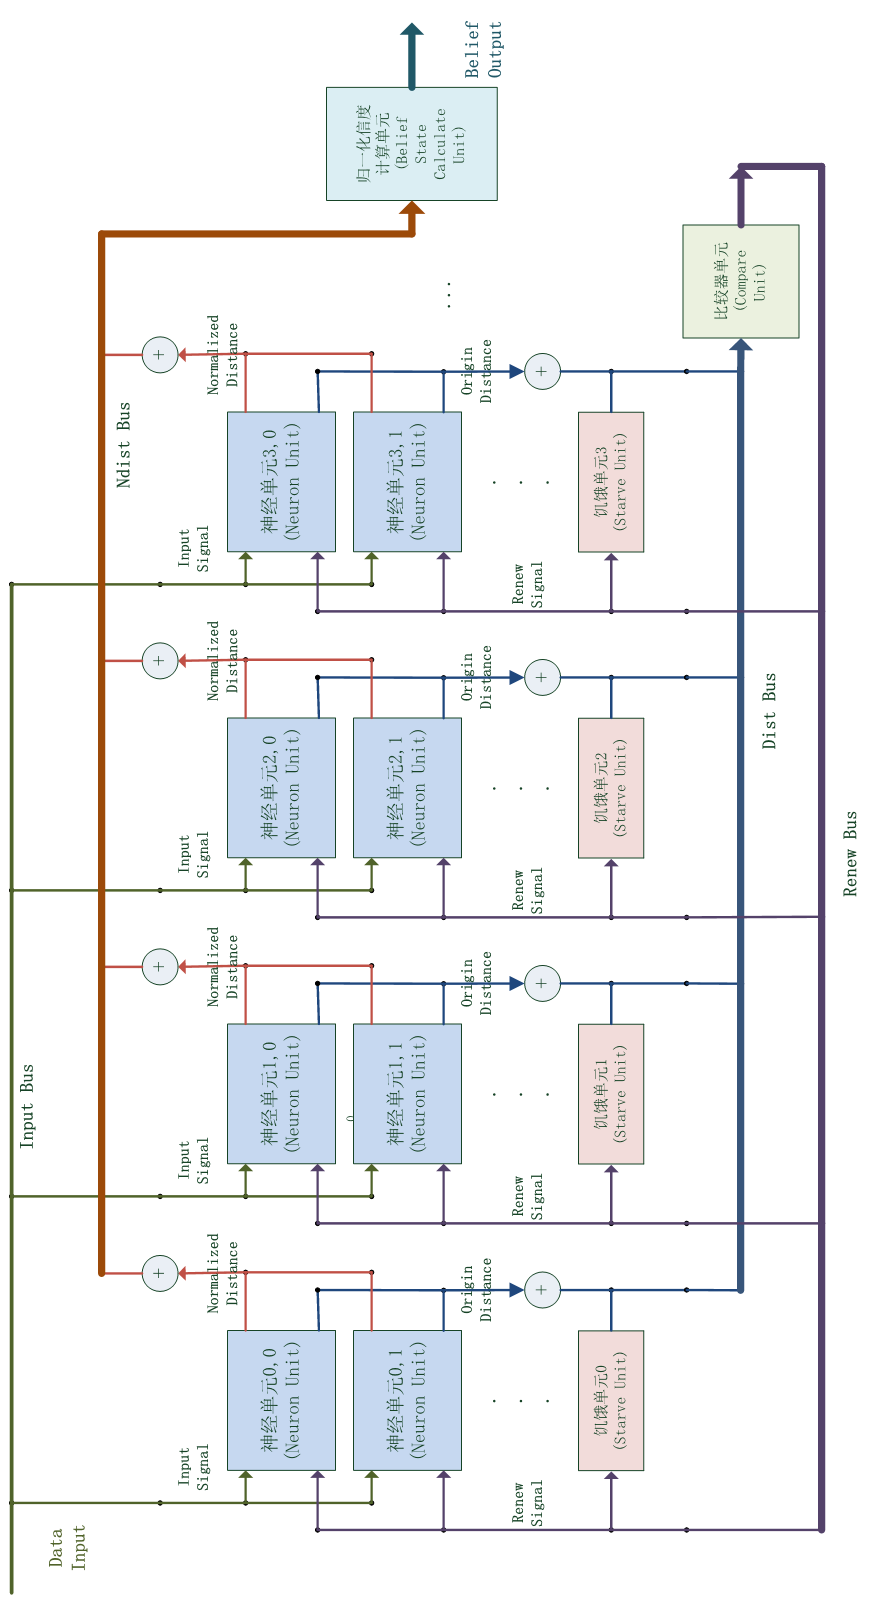
\includegraphics[width=0.8\textwidth]{ClusterStructure.png} % requires the graphicx package
   \caption{Online Clustering整体框架}
   \label{fig:clusterframe}
\end{figure}

\subsection{神经单元模块内部结构}
我们详细介绍神经单元Neuron Unit模块的设计。

如图\ref{fig:neuronunit},Neuron Unit外部引脚包括:
\begin{itemize}
\item 3个数据引脚(均为16bit):In, Mu-ini, Sigma2-ini,其中In接收观测数据输入,后面两个主要用于神经单元的参数初始化。

\item 3个使能端:En-input, En-renew, En-divide,分别进行其功能的主要阶段的控制:输入,计算dist;更新过程;计算ndist。使能端主要由外部的程序计数器控制(我们使用了有限状态机的方法)。

\item 2个判断信号: Ini-para, Renew-flag, 前一个用于是否初始化mu,sigma2的判断与信号选择;后一个由比较器返回,用于判断本次操作是否更新聚类参数mu,sigma2。

\item 2个底部引脚: Rst,Clk,其中一个为重置信号,另一个为时钟信号。

\item 3个输出引脚: Dist为单维度Euclid距离值输出;Ndist为单维度归一化Euclid距离值输出;Divide-flag为除法完成信号,用于后续步骤的指示。
\end{itemize}



\begin{figure}[htbp]
   \centering
   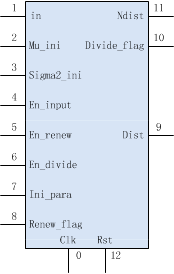
\includegraphics[width=0.2\textwidth]{NeuronUnit.png} % requires the graphicx package
   \caption{Neuron Unit外部引脚示意图}
   \label{fig:neuronunit}
\end{figure}

我们将其内部结构的实现通过Visio画出来,见\ref{fig:neuronunitlarge}。其中标注有“reg”的为内存器结构,上方引脚信号为使能端;“?”为路径选择器结构,上方引脚信号为选通信号;所有尖角正方形代表其为时序结构,底部引脚都要接上Rst,Clk;所有圆角或者圆形部分表示其为纯逻辑结构,应该在1个时钟周期内完成。

\begin{figure}[p]
   \centering
   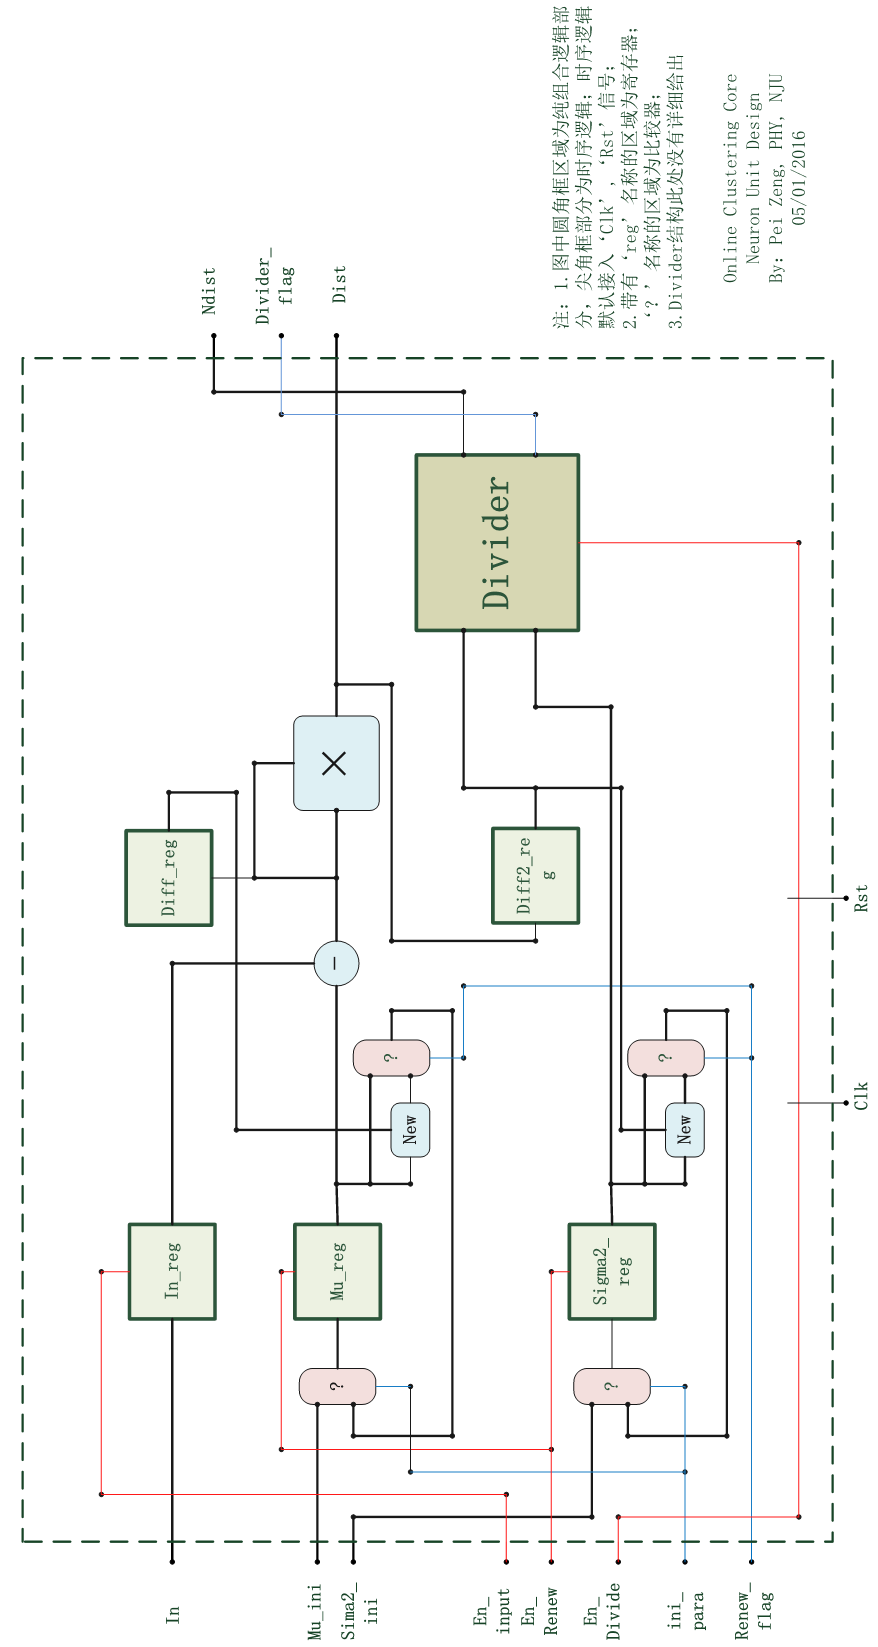
\includegraphics[width=0.8\textwidth]{NeuronUnitLarge.png} % requires the graphicx package
   \caption{Neuron Unit内部框架示意图}
   \label{fig:neuronunitlarge}
\end{figure}

我们不再详细介绍其他部分的结构,只将其Verilog代码附在附录里面。

\section{ModelSim仿真结果}
我们目前还没有完成对整个聚类的Modelsim仿真,只对每一个小部件进行了仿真。我们展示对于信度计算模块以及cordic除法器模块的仿真结果。

图\ref{fig:divsim}为除法器的仿真过程。我们测试了包括了正负数各种情况,较大与较小数相除等各种情况,确认了其除法的可靠性。(不能进行两个负数的除法;为了使其除法可靠,我们在除法器内部扩充了12位的辅助bit,参见附录Verilog代码)

\begin{figure}[htbp]
   \centering
   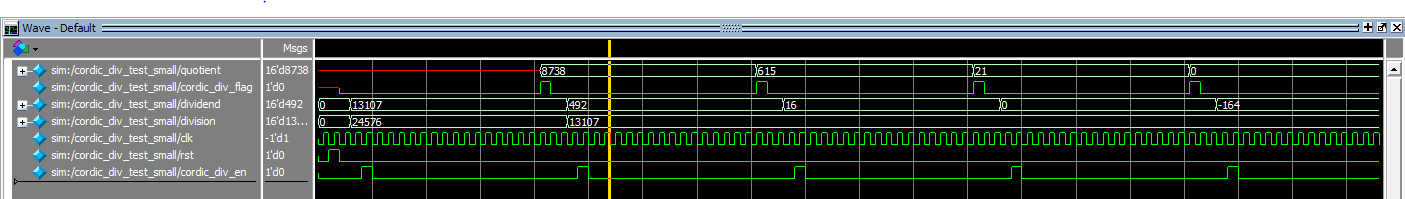
\includegraphics[width=0.8\textwidth]{DividerSim.png} % requires the graphicx package
   \caption{除法器的仿真结果}
   \label{fig:divsim}
\end{figure}


图\ref{fig:belisim}为信度计算模块的仿真过程。我们测试了十组参数,确认了其可靠信度计算的范围为:单个输入数据大于0.04,最高不超过1。(最高超过了影响不大,输入数据过小将导致结果错误)

\begin{figure}[htbp]
   \centering
   \includegraphics[width=0.8\textwidth]{BelicalSim.png} % requires the graphicx package
   \caption{信度计算的仿真结果}
   \label{fig:belisim}
\end{figure}

\subsection{现有问题与下一步的研究计划}
由于时间过短,笔者没有完成专用电路的整个设计流程。仍然有很多工作需要完成。

算法上,我们仍然没有解决特征空间位置移动时的时间空间特征识别的问题,我们将考虑结合卷积神经网络的方法,进行CTFAR测试以及动态识别的测试;

硬件上,我们仍然没有完成顶层模块的仿真工作(状态机设计有问题,数据量过于庞大);接下来我们要继续仿真工作,并进行综合排版布线,在FPGA上先进行测试,如果能够做到比较好的识别效果,可能会考虑进行流片工作。



\bibliography{reference}

%%%%%%%%%%%%%%%%%%%%%%%%%%%%%%%%%%%%%%%%%%%%%%%%%%%%%%%%%%%%%%%%%%%%%%%%%%%%%%%
% 致谢,应放在结论之后
\begin{acknowledgement}
%粗略版的
感谢大学四年期间帮助过我的所有老师,同学!

感谢父母尊重我的选择和一贯鼓励的态度!

感谢答辩期间林军老师、陈凯老师的指导与讨论!

感谢室友的互帮互助,鼓励支持!

感谢大学前三年给予了我莫大指导的王思慧老师,周慧君老师!

感谢在物理学院指导了我两年时间的王漱明老师!

感谢汪华老师,刘洁老师的无微不至的关照!
\end{acknowledgement}


\chapter{附录}\label{chapter_appendix}
\graphicspath{{chapter5/figure/}}

鉴于部分代码过于冗长,笔者并不附出;笔者已将其托管到自己的Github上:(https://github.com/qubiter),有兴趣可以前去访问。

\section{第三章算法测试:MNIST数字识别MATLAB代码}
\begin{spacing}{1}
\begin{lstlisting}[language=Matlab][deletekeywords={input, beta, gamma}]
%% DeSTIN Algorithm
%% STEP I: DeSTIN Network Training
%% Data Input
% the MNIST data is included in the MNIST.mat, where the X is the training
% image, y is the corresponding label.
load('MNIST.mat');

% Select Picture for Training
T = 5000; % Training Sample Number
sel = randperm(size(X, 1));
sel = sel(1:T);

% Display data
% Used the displayData.m function
displayData(X(sel,1:400))

fprintf('Program paused. Press enter to continue.\n');
%pause;

%% Initializing

% Online Clustering Learning Rate
alpha = 0.05; beta = 0.05;

% Starvation Rate
gamma = 0.992;

%{
Parameters for one neuron: 
1. Centroid attributes: mu, sigma2:   I-by-J matrix
2. Belief State:   J-by-1 vector
3. Input data:     I-by-1 vector
4. Starvation Trace:   J-by-1 vector
%}

% We adopt 'struct' structure for each neuron
Dim_Neu = [125, 125, 41; 25, 25, 25];
for k = 1:3
    for i = 1:2^(k-1)
        for j = 1:2^(k-1)
            n = (4^(k-1)-1)/3+(2^(k-1))*(i-1)+j;
            Neuron(n).input = zeros(Dim_Neu(1,k),1);
            Neuron(n).belief = zeros(Dim_Neu(2,k),1);
            Neuron(n).mu = 0.4 + 0.2 * rand(Dim_Neu(1,k),Dim_Neu(2,k));
            Neuron(n).sigma2 = ones(Dim_Neu(1,k),Dim_Neu(2,k));
            Neuron(n).starve = ones(Dim_Neu(2,k),1);
        end
    end
end

%% DeSTIN Training Process
% turn on the Training switch
training = 1;

% set a 'scanning sequence' for the MNIST data
scan = [0,0;0,1;0,2;0,3;0,4;1,4;1,3;1,2;1,1;1,0;2,0;2,1;...
2,2;2,3;2,4;3,4;3,3;3,2;3,1;3,0;4,0;4,1;4,2;4,3;4,4];
S = size(scan,1);
  
for t = 1:T % training sample sequence
    sample = reshape(X(sel(t),:), 20, 20);
    % scanning the sample with the specific sequence
    for s = 1:S  %scanning sequence
        sx = scan(s,1); sy = scan(s,2);
        for k = 3:-1:1  %for different layer
            for i = 1:2^(k-1)  % x label
                for j = 1:2^(k-1) % y label
                    n = (4^(k-1)-1)/3+(2^(k-1))*(i-1)+j; % calculating the neuron order number
                    if s == 1
                        Neuron(n).belief = 0.1 * ones(Dim_Neu(2,k),1); % reset the belief state at the beginning of each scanning; the belief state will be re-scaled later
                    end
                    % data transition
                    if k == 3  % for the bottom layer
                        A = reshape(sample(4*i-3+sx:4*i+sx,4*j-3+sy:4*j+sy),16,1);
                        % scaling the belief according to samle's mean value
                        Neuron(n).belief = Neuron(n).belief * ( mean(sample(:))./mean(Neuron(n).belief(:)) );
                        % input signal = spatial input + feedback input
                        Neuron(n).input = [A ; Neuron(n).belief];
                    else   % for the upper layer
                        % the spatial input from lower layer
                        B = [Neuron(((4^k-1)/3+2^k*((2*i-1-1)))+(2*j-1)).belief;...
                            Neuron(((4^k-1)/3+2^k*((2*i-1-1)))+(2*j)).belief;...
                            Neuron(((4^k-1)/3+2^k*((2*i-1)))+(2*j-1)).belief;...
                            Neuron(((4^k-1)/3+2^k*((2*i-1)))+(2*j)).belief];
                        %scaling
                        Neuron(n).belief = Neuron(n).belief * ( mean(sample(:))./mean(Neuron(n).belief(:)) );
                        Neuron(n).input = [B ; Neuron(n).belief];
                    end
                    % DeSTIN learning process
                    % Used the OnlineClustering function
                    [Neuron(n).belief,Neuron(n).mu,Neuron(n).sigma2,Neuron(n).starve] = OnlineClustering(...
                        Neuron(n).input,Neuron(n).mu,Neuron(n).sigma2,Neuron(n).starve, alpha,beta,gamma,training);
                end
            end
        end
    end
end

fprintf('Training completed. Press enter to continue.\n');
%pause;

%% Step II: 2-layer Neural Network Training
%% Sample Rechoose
T = 5000; % Neural Network Training sample number
sel = randperm(size(X, 1));
sel = sel(1:T);

% Display data
displayData(X(sel,1:400))

fprintf('Program paused. Press enter to continue.\n');
%pause;

%% DeSTIN usage: Acquire the output belief
% Turn off the training switch
training = 0;

% DeSTIN Learning Process
% belief state output to be collected
Belief = zeros(T, 21, 100);
for t = 1:T
    sample = reshape(X(sel(t),:), 20, 20);
    % scanning the sample with the specific sequence
    for s = 1:S
        sx = scan(s,1); sy = scan(s,2);
        for k = 3:-1:1
            for i = 1:2^(k-1)
                for j = 1:2^(k-1)
                    n = (4^(k-1)-1)/3+(2^(k-1))*(i-1)+j;
                    if s == 1
                        Neuron(n).belief = 0.1 * ones(Dim_Neu(2,k),1);
                    end
                    % data transition
                    if k == 3
                        A = reshape(sample(4*i-3+sx:4*i+sx,4*j-3+sy:4*j+sy),16,1);
                        % scaling
                        Neuron(n).belief = Neuron(n).belief * ( mean(sample(:))./mean(Neuron(n).belief(:)) );
                        Neuron(n).input = [A ; Neuron(n).belief];
                    else
                        B = [Neuron(((4^k-1)/3+2^k*((2*i-1-1)))+(2*j-1)).belief;...
                            Neuron(((4^k-1)/3+2^k*((2*i-1-1)))+(2*j)).belief;...
                            Neuron(((4^k-1)/3+2^k*((2*i-1)))+(2*j-1)).belief;...
                            Neuron(((4^k-1)/3+2^k*((2*i-1)))+(2*j)).belief];
                        %scaling
                        Neuron(n).belief = Neuron(n).belief * ( mean(sample(:))./mean(Neuron(n).belief(:)) );
                        Neuron(n).input = [B ; Neuron(n).belief];
                    end
                    % DeSTIN learning process
                    [Neuron(n).belief,Neuron(n).mu,Neuron(n).sigma2,Neuron(n).starve] = OnlineClustering(...
                        Neuron(n).input,Neuron(n).mu,Neuron(n).sigma2,Neuron(n).starve, alpha,beta,gamma,training);
                    % belief state storage
                    if mod(s,6) == 0
                       % Concatenate the 6,12,18,24th Belief state for storage
                       Belief(t,n,25*fix(s/6)-24:25*fix(s/6)) = (Neuron(n).belief)';
                    end
                end
            end
        end
 %{
        % **OUTPUT BELIEF STATE STORAGE
        % Collect the Belief output of specific position
        if mod(s,6)==0
            % Concatenate the 6,12,18,24th Belief state for storage
            Belief(t,25*fix(s/6)-24:25*fix(s/6)) = (Neuron(1).belief)'; 
        end
%}
    end
end

Belief = reshape(Belief,T,2100);
fprintf('Learning completed. Press enter to continue.\n');
%pause;

%% Initialize the Neural Network Parameters
input_layer_size  = 2100;   % Input Images of Neuron output
hidden_layer_size = 169;   % 20 hidden units
num_labels = 10;          % 10 labels, from 1 to 10  (note that we have mapped "0" to label 10)

% Weight Parameter for the 2-layer neural network
initial_Theta1 = randInitializeWeights(input_layer_size, hidden_layer_size);
initial_Theta2 = randInitializeWeights(hidden_layer_size, num_labels);
% Unroll parameters 
initial_nn_params = [initial_Theta1(:) ; initial_Theta2(:)];

% Regularization Factor
lambda = 1;

%% Neural Network Training
% Iteration options
options = optimset('MaxIter', 200);

% Create "short hand" for the cost function to be minimized
costFunction = @(p) nnCostFunction(p, ...
                                   input_layer_size, ...
                                   hidden_layer_size, ...
                                   num_labels, Belief, y(sel), lambda);

% Convex Optimization
[nn_params, cost] = fmincg(costFunction, initial_nn_params, options);

% Obtain Theta1 and Theta2 back from nn_params
Theta1 = reshape(nn_params(1:hidden_layer_size * (input_layer_size + 1)), ...
                 hidden_layer_size, (input_layer_size + 1));

Theta2 = reshape(nn_params((1 + (hidden_layer_size * (input_layer_size + 1))):end), ...
                 num_labels, (hidden_layer_size + 1));

fprintf('Program paused. Press enter to continue.\n');
%pause;

% Visualize the weight
%fprintf('\nVisualizing Neural Network... \n')

%displayData(Theta1(:, 2:end));

fprintf('\nProgram paused. Press enter to continue.\n');
%pause;

%% STEP III : Predictment Judge
%% Select Picture for Prediction
T = 1000; % Prediction Sample Number
sel = randperm(size(X, 1));
sel = sel(1:T);

%% Belief Calculation
% DeSTIN Learning Process
% belief state output to be collected
% exactly as the former DeSTIN part
training = 0;
Belief = zeros(T,21,100);
for t = 1:T
    sample = reshape(X(sel(t),:), 20, 20);
    % scanning the sample with the specific sequence
    for s = 1:S
        sx = scan(s,1); sy = scan(s,2);
        for k = 3:-1:1
            for i = 1:2^(k-1)
                for j = 1:2^(k-1)
                    n = (4^(k-1)-1)/3+(2^(k-1))*(i-1)+j;
                    if s == 1
                        Neuron(n).belief = 0.1 * ones(Dim_Neu(2,k),1);
                    end
                    % data transition
                    if k == 3
                        A = reshape(sample(4*i-3+sx:4*i+sx,4*j-3+sy:4*j+sy),16,1);
                        % scaling
                        Neuron(n).belief = Neuron(n).belief * ( mean(sample(:))./mean(Neuron(n).belief(:)) );
                        Neuron(n).input = [A ; Neuron(n).belief];
                    else
                       B = [Neuron(((4^k-1)/3+2^k*((2*i-1-1)))+(2*j-1)).belief;...
                            Neuron(((4^k-1)/3+2^k*((2*i-1-1)))+(2*j)).belief;...
                            Neuron(((4^k-1)/3+2^k*((2*i-1)))+(2*j-1)).belief;...
                            Neuron(((4^k-1)/3+2^k*((2*i-1)))+(2*j)).belief];
                        %scaling
                        Neuron(n).belief = Neuron(n).belief * ( mean(sample(:))./mean(Neuron(n).belief(:)) );
                        Neuron(n).input = [B ; Neuron(n).belief];
                    end
                    % DeSTIN learning process
                    [Neuron(n).belief,Neuron(n).mu,Neuron(n).sigma2,Neuron(n).starve] = OnlineClustering(...
                        Neuron(n).input,Neuron(n).mu,Neuron(n).sigma2,Neuron(n).starve, alpha,beta,gamma,training);
                    % belief state storage
                    if mod(s,6) == 0
                       % Concatenate the 6,12,18,24th Belief state for storage
                       Belief(t,n,25*fix(s/6)-24:25*fix(s/6)) = (Neuron(n).belief)';
                    end
                end
            end
        end
        %{
        % Collect the Belief output of specific position
        if mod(s,6)==0
            Belief(t,25*fix(s/6)-24:25*fix(s/6)) = (Neuron(1).belief)'; 
        end
        %}
    end
end
Belief = reshape(Belief,T,2100);
% Used perdict.m script
pred = predict(Theta1, Theta2, Belief);
fprintf('\nTraining Set Accuracy: %f\n', mean(double(pred == y(sel))) * 100);
toc;


\end{lstlisting}
\end{spacing}


\section{第四章硬件设计:部分Verilog代码}
\subsection{NeuronUnit:框架代码}
\begin{spacing}{1}
\begin{lstlisting}[language=Verilog]
`timescale 1ns / 100ps

module neuronunit(dist, norm_dist, divider_flag, in, mu_ini, sigma2_ini, en_input, en_renew, en_divide, renew_flag, ini_para, clk, rst);
  output signed [15:0] dist;
  output signed [15:0] norm_dist;
  output divider_flag; //divider_flag
  input signed [15:0] in;
  input signed [15:0] mu_ini;
  input signed [15:0] sigma2_ini;
  input en_input; //sample input control
  input en_renew; //renew process indicator
  input en_divide; //divider work signal
  input renew_flag; //whether new value or old one
  input ini_para; //for mu sigma2 initialization
  input clk;
  input rst;
  
  reg signed [15:0] in_reg;
  reg signed [15:0] mu;
  reg signed [15:0] sigma2;
  reg signed [15:0] diff_reg;
  reg signed [15:0] diff2_reg;
  //reg signed [15:0] dist;
  //reg signed [15:0] norm_dist;
  //reg divider_flag; //divider flag
  
  wire signed [15:0] diff;
  wire signed [15:0] diff2;
  wire signed [15:0] mu0;
  wire signed [15:0] sigma20;
  wire signed [15:0] mu_new;
  wire signed [15:0] sigma2_new;
  ///wire signed  [15:0] diff2_diff; //diff2_reg - sigma2
  wire divider_flag;
  
  //mu,sigma2 data input control
  assign mu0 = ini_para? mu_ini : mu_new;
  assign sigma20 = ini_para? sigma2_ini : sigma2_new;
  
  //pure logical calculation
  assign diff = in_reg - mu;
  assign dist = diff2;
  //pure logical multiplier
  fixed_width_multiply_16bits multiplier(.a(diff), .b(diff), .c(diff2));
  
  //renew rule execution
  assign mu_new = renew_flag? (mu + (diff_reg >>> 3 )) : mu;
  ///assign diff2_diff = diff2_reg - sigma2;
  assign sigma2_new = renew_flag? (sigma2 + (diff2_reg - sigma2) / 8 ) : sigma2;
  
  //examplify the divider
  cordic_div_smaller divider(.cordic_div_flag(divider_flag),.quotient(norm_dist),.dividend(diff2_reg),.division(sigma2),.clk(clk),.rst(rst),.cordic_div_en(en_divide));
  
  //register transition description
  always @(posedge clk or posedge rst)
  begin
    if (rst) begin in_reg = 16'd0; mu = 16'd0; sigma2 = 16'd0; diff_reg = 16'd0; diff2_reg = 16'd0; /*divider_flag = 0; norm_dist = 16'd0;*/ end
    else
      begin
        //diff,diff2 to register
        diff_reg <= diff;
        diff2_reg <= diff2;
        
        //input register renew
        if (en_input) in_reg <= in;
        
        //mu sigma2 register renew
        if (en_renew || ini_para) begin mu <= mu0; sigma2 <= sigma20; end
      end
  end
endmodule
\end{lstlisting}
\end{spacing}

\subsection{NeuronUnit:测试代码}

\begin{spacing}{1}
\begin{lstlisting}[language=Verilog]
`timescale 1ns / 100ps

module neuronunit_test();
  
  
  wire signed [15:0] dist;
  wire signed [15:0] norm_dist;
  wire divider_flag;
  
  reg clk;
  reg rst;
  reg en_input;
  reg en_renew;
  reg en_divide;
  reg renew_flag;
  reg ini_para;
  
  reg signed [15:0] in;
  reg signed [15:0] mu_ini;
  reg signed [15:0] sigma2_ini;
  
  
  neuronunit neuronunit_exam(.dist(dist), .norm_dist(norm_dist), .divider_flag(divider_flag), .in(in), .mu_ini(mu_ini), .sigma2_ini(sigma2_ini), 
  .en_input(en_input), .en_renew(en_renew), .en_divide(en_divide), .renew_flag(renew_flag), .ini_para(ini_para), .clk(clk), .rst(rst));
  
  initial
  begin
    // initialzation
    clk = 0;
    rst = 0;
    en_input = 0;
    en_renew = 0;
    en_divide = 0;
    renew_flag = 0;
    ini_para = 0;
    in = 0;
    mu_ini = 0;
    sigma2_ini = 0;
    
    // reset
    #10
    rst = 1;
    #10
    rst = 0;
    
    // initialize mu, sigma2: 0.5, 1
    #10
    ini_para = 1;
    #10
    mu_ini = 8192;
    sigma2_ini = 16384;
    #10
    ini_para = 0;
    mu_ini = 0;
    sigma2_ini = 0;
    
    // 1st input:0
    #10
    in = 0;
    #10
    en_input = 1;
    #10
    en_input = 0;
    
    // 1st renew part
    #10
    renew_flag = 1;
    #10
    en_renew = 1;
    #10
    en_renew = 0;
    
    // 1st divide part
    #10
    en_divide = 1;
    #10
    en_divide = 0;
    #140
    
    
    // 2nd input:0
    #10
    in = 0;
    #10
    en_input = 1;
    #10
    en_input = 0;
    
    // 2nd renew part
    #10
    renew_flag = 0;
    #10
    en_renew = 1;
    #10
    en_renew = 0;
    
    // 2nd divide part at least #140
    #10
    en_divide = 1;
    #10
    en_divide = 0;
    #140
    
    // 3rd input:0.2
    #10
    in = 3277;
    #10
    en_input = 1;
    #10
    en_input = 0;
    
    // 3rd renew part
    #10
    renew_flag = 1;
    #10
    en_renew = 1;
    #10
    en_renew = 0;
    
    // 3rd divide part at least #140
    #10
    en_divide = 1;
    #10
    en_divide = 0;
    #140

    #100
    $stop;
  end
  
  //clock
  initial
  begin
  forever
    #5 clk = ~clk;
  end
endmodule

\end{lstlisting}
\end{spacing}


\subsection{Cordic除法器:框架代码}
\begin{spacing}{1}
\begin{lstlisting}[language=Verilog]
`timescale 1ns / 100ps
module cordic_div_smaller(cordic_div_flag, quotient, dividend, division, clk, rst, cordic_div_en);
  parameter M = 1 ; // dividend shift bits (<<) 
  parameter N = 13; // division shift bits (>>) M + N = FractionLength
  parameter COUNT = 14; //Maximum count number
  
  output reg signed [15:0] quotient;
  output reg cordic_div_flag;
  
  input signed [15:0] dividend;
  input signed [15:0] division;
  input clk;
  input rst;
  input cordic_div_en;
  
  reg signed [43:0] y; //if result collapsed,try to alloc more bits.
  wire signed [43:0] y_buf;
  wire signed [27:0] y_mv;
  wire signed [27:0] y_mv2;
  
  reg [27:0] x;
  wire signed [27:0] x_mv;
  wire signed [27:0] x_mv2;
  
  reg signed [15:0] z;
  
  integer count;
  integer state;
  
  //extend the dividend's bit number
  assign y_mv = {dividend, 12'h0};
  assign y_mv2 = y_mv <<< M;  // redifine y_mv to get a right representation of z
  assign x_mv = {division, 12'h0};
  assign x_mv2 = x_mv >>> N;  // redifine x_mv to get a right representation of z
  assign y_buf = (y_mv2[27])?{16'hffff, y_mv2}:{16'h0000, y_mv2}; 
  
  always@(posedge clk or negedge rst)
  begin
    if(rst)begin
      state <= 0;
      count <= COUNT;
      x <= 0;
      y <= 0;
      z <= 0;
    end
    else begin
      case(state)
        0: begin
          cordic_div_flag <= 0;
          if(cordic_div_en) begin
            x <= x_mv2;
            y <= y_buf;
            z <= 0;
            state <= 1;
          end
        end
        1: begin
          if(count >= 0)begin
            count <= count - 1;
            if(y==0)begin
              y <= y;
              z <= z;
            end
            else if(y<0)begin
              z <= z - (1<<count);
              y <= y + (x<<count);
            end
            else begin
              z <= z + (1<<count);
              y <= y - (x<<count);
            end 
          end
          else begin
            count <= COUNT;
            quotient <= z;
            cordic_div_flag <= 1;
            state <= 0;
          end
        end
      endcase
    end
  end
  
endmodule

\end{lstlisting}
\end{spacing}


\subsection{Cordic除法器:测试代码}
\begin{spacing}{1}
\begin{lstlisting}[language=Verilog]
`timescale 1ns / 100ps

module cordic_div_test_small();
  
  
  wire signed [15:0] quotient;
  wire cordic_div_flag;
  
  reg signed [15:0] dividend;
  reg signed [15:0] division;
  reg clk;
  reg rst;
  reg cordic_div_en;
  cordic_div_smaller div_exam(.cordic_div_flag(cordic_div_flag), .quotient(quotient), .dividend(dividend), .division(division), .clk(clk), .rst(rst), .cordic_div_en(cordic_div_en));
  
  initial
  begin
    clk = 0;
    rst = 0;
    cordic_div_en = 0;
    dividend = 0;
    division = 0;
    #10
    rst = 1;
    #10
    rst = 0;
    // 1st: 0.8/1.5  8738
    #10
    dividend = 13107;
    division = 24576;
    #10
    cordic_div_en = 1;
    #10
    cordic_div_en = 0;
    // 2nd: 0.03/0.8  629
    #180
    dividend = 492;
    division = 13107;
    #10
    cordic_div_en = 1;
    #10
    cordic_div_en = 0;
    // 3rd: 0.001/0.8  21
    #180
    dividend = 16;
    division = 13107;
    #10
    cordic_div_en = 1;
    #10
    cordic_div_en = 0;
    // 4th: 0.00001/0.8  0
    #180
    dividend = 0;
    division = 13107;
    #10
    cordic_div_en = 1;
    #10
    cordic_div_en = 0;
    // 5th: -0.01/0.8  -209
    #180
    dividend = -164;
    division = 13107;
    #10
    cordic_div_en = 1;
    #10
    cordic_div_en = 0;
    // 6th: 0.024/0.049  7809
    #180
    dividend = 393;
    division = 817;
    #10
    cordic_div_en = 1;
    #10
    cordic_div_en = 0;
    
    #200
    $stop;
  end
  initial
  begin
  forever
    #5 clk = ~clk;
  end
endmodule
\end{lstlisting}
\end{spacing}
%%%%%%%%%%%%%%%%%%%%%%%%%%%%%%%%%%%%%%%%%%%%%%%%%%%%%%%%%%%%%%%%%%%%%%%%%%%%%%%
\end{document}
